%% ut-thesis.tex -- document template for graduate theses at UofT
%%
%% Copyright (c) 1998-2012 Francois Pitt <fpitt@cs.utoronto.ca>
%% last updated at 09:43 (EDT) on Fri  1 Jun 2012
%%
%% This work may be distributed and/or modified under the conditions of
%% the LaTeX Project Public License, either version 1.3c of this license
%% or (at your option) any later version.
%% The latest version of this license is in
%%     http://www.latex-project.org/lppl.txt
%% and version 1.3c or later is part of all distributions of LaTeX
%% version 2005/12/01 or later.
%%
%% This work has the LPPL maintenance status "maintained".
%%
%% The Current Maintainer of this work is
%% Francois Pitt <fpitt@cs.utoronto.ca>.
%%
%% This work consists of the files listed in the accompanying README.

%% SUMMARY OF FEATURES:
%%
%% All environments, commands, and options provided by the `ut-thesis'
%% class will be described below, at the point where they should appear
%% in the document.  See the file `ut-thesis.cls' for more details.
%%
%% To explicitly set the pagestyle of any blank page inserted with
%% \cleardoublepage, use one of \clearemptydoublepage,
%% \clearplaindoublepage, \clearthesisdoublepage, or
%% \clearstandarddoublepage (to use the style currently in effect).
%%
%% For single-spaced quotes or quotations, use the `longquote' and
%% `longquotation' environments.


%%%%%%%%%%%%         PREAMBLE         %%%%%%%%%%%%

%%  - Default settings format a final copy (single-sided, normal
%%    margins, one-and-a-half-spaced with single-spaced notes).
%%  - For a rough copy (double-sided, normal margins, double-spaced,
%%    with the word "DRAFT" printed at each corner of every page), use
%%    the `draft' option.
%%  - The default global line spacing can be changed with one of the
%%    options `singlespaced', `onehalfspaced', or `doublespaced'.
%%  - Footnotes and marginal notes are all single-spaced by default, but
%%    can be made to have the same spacing as the rest of the document
%%    by using the option `standardspacednotes'.
%%  - The size of the margins can be changed with one of the options:
%%     . `narrowmargins' (1 1/4" left, 3/4" others),
%%     . `normalmargins' (1 1/4" left, 1" others),
%%     . `widemargins' (1 1/4" all),
%%     . `extrawidemargins' (1 1/2" all).
%%  - The pagestyle of "cleared" pages (empty pages inserted in
%%    two-sided documents to put the next page on the right-hand side)
%%    can be set with one of the options `cleardoublepagestyleempty',
%%    `cleardoublepagestyleplain', or `cleardoublepagestylestandard'.
%%  - Any other standard option for the `report' document class can be
%%    used to override the default or draft settings (such as `10pt',
%%    `11pt', `12pt'), and standard LaTeX packages can be used to
%%    further customize the layout and/or formatting of the document.

%% *** Add any desired options. ***
\documentclass{ut-thesis}

%% *** Add \usepackage declarations here. ***
%% The standard packages `geometry' and `setspace' are already loaded by
%% `ut-thesis' -- see their documentation for details of the features
%% they provide.  In particular, you may use the \geometry command here
%% to adjust the margins if none of the ut-thesis options are suitable
%% (see the `geometry' package for details).  You may also use the
%% \setstretch command to set the line spacing to a value other than
%% single, one-and-a-half, or double spaced (see the `setspace' package
%% for details).

\usepackage{amsmath}

\usepackage{graphicx}
\usepackage{caption}
\usepackage{subcaption}

\usepackage{float}
\usepackage{epstopdf}

\usepackage{hyperref}

\usepackage{multirow}

%%%%%%%%%%%%%%%%%%%%%%%%%%%%%%%%%%%%%%%%%%%%%%%%%%%%%%%%%%%%%%%%%%%%%%%%
%%                                                                    %%
%%                   ***   I M P O R T A N T   ***                    %%
%%                                                                    %%
%%  Fill in the following fields with the required information:       %%
%%   - \degree{...}       name of the degree obtained                 %%
%%   - \department{...}   name of the graduate department             %%
%%   - \gradyear{...}     year of graduation                          %%
%%   - \author{...}       name of the author                          %%
%%   - \title{...}        title of the thesis                         %%
%%%%%%%%%%%%%%%%%%%%%%%%%%%%%%%%%%%%%%%%%%%%%%%%%%%%%%%%%%%%%%%%%%%%%%%%

%% *** Change this example to appropriate values. ***
\degree{M.A.Sc}
\department{IBBME}
\gradyear{2015}
\author{Di Xue}
\title{Exploring the Feasibility of Prompting Daily Task Execution using the NAO Humanoid Robot with Children with Autism Spectrum Disorder}

%% *** NOTE ***
%% Put here all other formatting commands that belong in the preamble.
%% In particular, you should put all of your \newcommand's,
%% \newenvironment's, \newtheorem's, etc. (in other words, all the
%% global definitions that you will need throughout your thesis) in a
%% separate file and use "\input{filename}" to input it here.


%% *** Adjust the following settings as desired. ***

%% List only down to subsections in the table of contents;
%% 0=chapter, 1=section, 2=subsection, 3=subsubsection, etc.
\setcounter{tocdepth}{2}

%% Make each page fill up the entire page.
\flushbottom


%%%%%%%%%%%%      MAIN  DOCUMENT      %%%%%%%%%%%%

\begin{document}

%% This sets the page style and numbering for preliminary sections.
\begin{preliminary}

%% This generates the title page from the information given above.
\maketitle

%% There should be NOTHING between the title page and abstract.
%% However, if your document is two-sided and you want the abstract
%% _not_ to appear on the back of the title page, then uncomment the
%% following line.
%\cleardoublepage

% This generates the abstract page, with the line spacing adjusted
% according to SGS guidelines.
\begin{abstract}
%% *** Put your Abstract here. ***
This thesis seeks to improve the state of the art prompting system, COACH, for the children with ASD population.  It investigates the prospects of using a humanoid robot, NAO, as its prompting agent through a Wizard of Oz (WoZ) pilot study, and it explores the feasibility of using a 3D camera, Kinect, to implement a Visual Focus of Attention (VFOA) tracker that enables COACH to know if the child is engaged in the activity.  The WoZ study showed promising results of the robot's ability to assist a child with ASD through hand-washing tasks.  It also suggested that parent robot joint prompting sessions as a valid method for improving child's compliance to the robot.  On the other hand, the implementation of the VFOA tracker was half completed.  Of the three component of the VFOA tracker (namely head pose tracking, eye pose tracking, object under gaze identification), only a head pose tracker and an object under gaze identifier were implemented.  The head tracker performed under normal head movements, but had limited success with the child with ASD participant during hand-washing, due to the child's rocking back and forth rapidly.  A simple Gaussian ellipsoid object location calibration method was implemented for the object under gaze identifier.
%% (At most 150 words for M.Sc. or 350 words for Ph.D.)
\end{abstract}

%% Anything placed between the abstract and table of contents will
%% appear on a separate page since the abstract ends with \newpage and
%% the table of contents starts with \clearpage.  Use \cleardoublepage
%% for anything that you want to appear on a right-hand page.

% This generates a "dedication" section, if needed
% (uncomment to have it appear in the document).
%\begin{dedication}.
% *** Put your Dedication here. ***
\section*{Dedication}
I would like to dedicate this thesis to my family -- your love, your patience, and your encouragements were the sources of my strength in this prolonged course of my study.
%\end{dedication}

%% The `dedication' and `acknowledgements' sections do not create new
%% pages so if you want the two sections to appear on separate pages,
%% you should put an explicit \newpage between them.

% This generates an "acknowledgements" section, if needed
% (uncomment to have it appear in the document).
%\begin{acknowledgements}
%% *** Put your Acknowledgements here. ***
\section*{Acknowledgments}
First, I would like to thank my supervisor, Alex Mihailidis, for his support, guidance, and kindness, through out my thesis.  In all the turning points of my thesis, he had always put my interest first.  He was patient, kind, and an expert in many research areas.  I am very grateful for knowing him as my supervisor.

I would also want to thank Tuck-Voon How, Bing Ye, and Jennifer Boger, for being the fun and resourceful people they are.  They, along with other dear members of IATSL, always made my trip to the lab fun and fruitful.

I would like to thank Jiayang Jiang for his awesome depth first search code, and Leon for teaching me the power of Latex.  I also want to thank Jason, Maria, Harry, Boyuetty, Jimverley, Stephen, Jon, Dave, and PA, for being there for me to encourage me and to spur me on when time gets hard.

Last, but not least, I am grateful for the dear Brothers and Sisters at Crosspoint Fellowship.  Without you guys, I would not have made it.

Soli Deo Gloria!
%\end{acknowledgements}


\listoffigures
\listoftables


%% This generates the Table of Contents (on a separate page).
\tableofcontents

%% This generates the List of Tables (on a separate page), if needed
%% (uncomment to have it appear in the document).
%\listoftables

%% This generates the List of Figures (on a separate page), if needed
%% (uncomment to have it appear in the document).
%\listoffigures

%% You can add commands here to generate any other material that belongs
%% in the head matter (for example, List of Plates, Index of Symbols, or
%% List of Appendices).

%% End of the preliminary sections: reset page style and numbering.
\end{preliminary}


%%%%%%%%%%%%%%%%%%%%%%%%%%%%%%%%%%%%%%%%%%%%%%%%%%%%%%%%%%%%%%%%%%%%%%%%
%%  Put your Chapters here; the easiest way to do this is to keep     %%
%%  each chapter in a separate file and `\include' all the files.     %%
%%  Each chapter file should start with "\chapter{ChapterName}".      %%
%%  Note that using `\include' instead of `\input' will make each     %%
%%  chapter start on a new page, and allow you to format only parts   %%
%%  of your thesis at a time by using `\includeonly'.                 %%
%%%%%%%%%%%%%%%%%%%%%%%%%%%%%%%%%%%%%%%%%%%%%%%%%%%%%%%%%%%%%%%%%%%%%%%%


%% *** Include chapter files here. ***

\chapter{Introduction}


\section{Motivation}

\subsection{Children with ASD and the need for ATCs}

Autism spectrum disorder (ASD) is a complex neurological and developmental condition that is characterized by impairments in social communication and the presence of repetitive behaviours and restricted interests \cite{american2013diagnostic}.  Recent research suggested that the prevalence of ASD among children aged 8 years (the peak prevalence age), when the broad spectrum is considered, is as high as 1:68 in the United States \cite{baoi2014prevalence}.  Although there is no federal government monitoring system currently present in Canada that provides accurate estimate of its prevalence of ASD, we know that ASD is the most common form of neurological disorder and severe developmental disability in children \cite{autism2014facts}.

Some children with ASD may have difficulty in learning self-management skills and require continuous assistance from a caregiver to carry-out activities of daily living (ADLs).  Assistive technologies for cognition (ATCs) aim to assist, instruct, train, or educate individuals with cognitive disabilities to overcome challenges in life, including executing activities of daily living (ADL).  In particular, autonomous or self-operated ATCs promote independence for children with ASD in need of such assistance.  Commercially available devices such as computers, video players, audio players, cellphones, etc. have all been exploited as platforms for ATCs.


\subsection{COACH and its Challenges}

The COACH (Cognitive Orthosis for Assisting with aCtivites in the Home) system, developed by Mihailidis et al., is an autonomous prompting system \cite{mihailidis2008coach}.  It uses computer vision and artificial intelligence to automatically detect user actions when executing ADLs, and prompts appropriately when a user needs assistance.  It was first developed for the dementia population, but a version appropriate to the ASD population was recently adapted and tested in a pilot study \cite{bimbrahw2012investigating}.


The system currently uses audio and video prompts using an LCD monitor screen as its primary prompting modalities.  In the pilot study, the hand-washing activity is used as an example to test the system's effectiveness because of the simplicity of its tasks as well as the washroom settings being easily controlled.  The hand-washing activity is broken into five steps, with verbal prompts being: ``turn on the water and wet your hands'', ``put soap on your hands'', ``scrub your hands'', ``rinse your hands'', ``turn off the water and dry your hands''.  At each step, if the child does not successfully execute the correct action within a time threshold, the system prompts.  The prompting consist of first displaying a still image attention grabber on screen that attempts to capture child's attention, then playing the pre-recorded audio and/or video prompts.  The video prompts are videos recorded from point-of-view (first person) perspective of a person executing the step.  If child successfully executes a step with or without prompting, the system congratulates by saying ``Good job''.  If the child does not get it right within a time threshold, the system prompts again.  This is repeated until a predetermined maximum number of times before calling over the caregiver to assist.  


The pilot study of COACH for ASD showed good acceptance by the children with ASD and their caregivers \cite{bimbrahw2012investigating}.  System effectiveness was shown in that 78\% of the hand-washing steps were completed without caregiver assistances by the children themselves, all of whom were unable to wash-hands on their own before.


The major area of improvement identified in the study was to increase the child's engagement during prompting and task execution.  Firstly, almost half of the system's prompts were ignored by the children.  Assuming that these children were able to understand the prompts, as seen by their correct actions to the not ignored prompts, their noncompliance is a reflection of their disinterest in the prompts.  Secondly, several occasions of child being distracted or disinterested to tasks were observed.


To tackle this problem, two potential approaches can be applied: 1) change the prompting modality to one that's inherently more engaging to the child (e.g. humanoid robot); 2) track the child's visual focus of attention in real-time, and issue attention grabbers when child is distracted.

\section{Roadmap}

This thesis will address how to improve the visual focus of attention of children with ASD when prompted by COACH.  It will approach the problem by incorporating a humanoid robot, NAO, and implementing algorithms to track and react to the child's gaze, in attempts to better engage children during ADL prompting sessions.


The thesis report will be broken into the following sections:


In Chapter 2, we first review the relevant literature on the established frameworks for ASD interventions, especially those that teach skills of daily living, and relate it to our prompting framework.  Next, we review research for ASD interventions that utilize technologies such as videos, computers, and robots, confirming this thesis' approach and identifying the research gap.  Also, our research direction is put into context in the Human Robot Interaction (HRI) field.  Lastly, we review state of the art research in visual focus of attention estimation, targeting key methodologies appropriate for this thesis's goal.


In Chapter 3, the research objectives and hypotheses are summarized.

In Chapter 4, the Wizard of Oz pilot study is presented.  The study setup, protocol, data collected, analysis and results are discussed in details.

In Chapter 5, the investigated algorithms for tracking a person's visual focus of attention are presented.  Specifically, the problem is broken into head pose estimation, eye pose estimation, and object identification.  The methods and evaluation for each are discussed.

In Chapter 6, we summarize and conclude the thesis.




\chapter{Literature Review}

\section{ASD Interventions}

Currently, interventions are mainly aimed to help children with ASD adjust more effectively to their environment \cite{francis2005autism}.  There are many approaches to ASD interventions, such as behavior based, pharmaceutically based, or dietary based \cite{francis2005autism}.  Also, there are interventions that focus on specific problems a child may experience, such as augmentative communication therapy, social skills teaching, sensory integration therapy \cite{francis2005autism}.  One reason for such a diverse collection of therapies to exist is because of the varying nature of ASD disabilities across individuals, making one single method not effective for the whole population, and sometimes not sufficient for an individual.  Consequently, it remains a challenge to show effectiveness of a method in a clinically significant sense, even if it is truly effective to a small sample of the population.  The most clinically tested, commonly practiced, and recommended methods are those based on the principles of Applied Behaviour Analysis \cite{foxx2008applied}.


\subsection{Applied Behaviour Analysis and Early Intensive Behavior Intervention}
Applied Behaviour Analysis (ABA) is based on scientifically proven theories of human behaviors, and is widely used for treating inappropriate behaviors and teaching new behaviors.  Its strategies for treating inappropriate behaviors include: finding and changing antecedents to inappropriate behaviors, ignoring the behavior, or negative reinforcement through punishment \cite{foxx1982decreasing}.  Its strategies for teaching new behaviors include: giving stimuli to child to elicit a new behavior, positive reinforcement (e.g. praise), and maintenance and generalization strategies to make sure the newly learned behavior is retained across time and settings \cite{foxx1982decreasing}.  For cuing stimuli, high level of consistency is needed.  For positive reinforcement, individually selected and strategically used motivators (e.g. praise, a hug, a check mark, a favorite activity) should be given immediately after appropriate behaviors.  For maintenance and generalization strategies, prompt fading and testing across context and settings can be used.


For some children with ASD, research has shown that early ABA based intervention with intensive and extensive sessions of minimum 30 hours a week for 2 years (also known as Early Intensive Behavioral Intervention (EIBI)) are proven to be successful for improving ASD outcomes \cite{howlin2009systematic}.  Meta analyses have been conducted to evaluate the efficacy of EIBI for children with ASD.  Three meta-analyses \cite{eldevik2009meta, reichow2009comprehensive, peters2011meta} found that, for children with ASD participating in EIBI versus those receiving other treatments or treatment as usual, an average medium to large effect size can be observed for IQ change, which may be considered clinically significant \cite{hojat2004visitor}.  Both Eldevik et al. \cite{eldevik2009meta} and Peters-Scheffer et al. \cite{peters2011meta} also found that a smaller effect size for adaptive behavior change can be observed.  However, there are large individual differences in treatment response for children with ASD and most children continue to require specialized services \cite{thill2012robot}.  All in all though, EIBI is the standard of care for children with ASD in North America \cite{keenan2014autism}.

\subsection{Daily Living Skill Teaching and the Discrete Trial Training}
In many children and adults with ASD, daily living skills are one of the key skills that still need to be learned through training and interventions.  In a study for adults with high functioning ASD by \cite{farley2009twenty}, they found that, among a range of variables including IQ, adaptive behavior measures (Vineland Adaptive Behavior Scales -– VABS \cite{sparrow2005vineland}) were the variables most closely and positively related to better outcome. Across the adaptive domains the ‘daily living skills’ domain was most highly associated with better outcome of quality of life.

There are three major cognitive theories developed that attempt to explain the underlying mechanics of the difficulties experienced by individuals with ASD: Theory of Mind deficit, executive dysfunctioning, and weak central coherence \cite{rajendran2007cognitive}.  The Theory of Mind deficit explains some individuals with ASD's inability to create an image of an agent's mental states (including one's own), thus the inability to infer what others think, believe, and desire, consequently to predict their behaviors.  Executive dysfunctioning explains some individuals with ASD's impairments in several higher-level capacities necessary for planning and monitoring of behaviors, set shifting, inhibiting automatic actions, and holding information in working memory.  Weak central coherence explains some individuals with ASD's cognitive style of local or detail-focused processing, leading to missing more global processing of information in context and for meaning.  These cognitive impairments in individuals with ASD are the underlying factors that cause some individuals to have difficulties learning and executing activities of daily living.  One approach to address this is through cognitive function trainings that focus on learning isolated cognitive skills that the individual lacks.  It has been found, however, that improvements in adaptive behaviors may not automatically result in improvements in cognitive skills \cite{chin2000teaching, teunisse2007cognitieve}.  Thus, instead of targeting the cognitive skills, which might not generalize to adaptive behaviors, the more direct approach would be to target the behaviors themselves, through interventions such as those based on the ABA framework.

Discrete trial training (DTT) \cite{howard2005comparison}, incidental teaching (IT) \cite{mcgee1986extension}, and pivotal response training (PRT) \cite{koegel2003teaching} are interventions effectively used in adaptive skill building in children with ASD and are based on ABA methodology \cite{palmen2013behavioral}.  DTT focuses on specific targeted behaviors, and relies on intensive and repetitive trainings with appropriate and immediate reinforcements.  IT focuses on teaching the child through natural means, emphasizing on having the child initiate learning opportunities.  For example, the therapist may hide one of the shoes of the child before it is time to go outside, thus creating an opportunity for the child to request verbally the missing shoe.  PRT philosophy also emphasizes naturalistic teaching.  Instead of focusing on individual behaviors, it targets ``pivotal'' areas of the child's development, such as motivations, response to multiple cues, self-management, and initiation of social interactions.  By targeting these key pivotal areas for improvement, broad area improvements can be seen in sociability, communication, behavior, and academic skill building.

Reviewing these methods, DTT is the most appropriate for teaching skills for a single activity of daily living, such as teaching hand-washing.  Many studies have shown effectiveness of EIBI using DTT, as reviewed by Case-Smith et al. \cite{case2008evidence}: The original study of DTT, by Lovaas, compared two groups of 19 young children with ASD, one receiving 40 hours per week of intensive DTT and the other receiving 10 hours or less of similar training, and showed improved IQ for the former after 2 years of intervention \cite{lovaas1987behavioral}.  There are many studies that confirmed these findings.  For one, in a more recent study, Cohen et al. compared two groups of 21 children with ASD, one receiving EIBI for one year and moved to less intensive services after, the other group receiving community-based services only, and showed higher IQ, language comprehension, and adaptive behavior for the former group by the end of 3 years \cite{cohen2006early}.  In addition, the DTT method is reproducible by nonprofessionals, as well.  Sallows et al. showed that parents who are taught proper implementation of DTT produced similar results with children with ASD as those produced by trained therapists after 4 years \cite{sallows2005intensive}.

\subsubsection{Implementation Details of DTT}
In summary, there are five steps to DTT \cite{bogin2010steps}:
\begin{enumerate}
	\item \textbf{Grabbing the child's attention}
	\item \textbf{Discriminative stimulus}: must be simple, clear, and concise, and wording must be consistent
	\item \textbf{Child's response}: if the child's response is incorrect, stop it by instructing again immediately or provide prompts
	\item \textbf{Prompt to aid the child if no response or wrong}: this has the advantage of helping him quickly move through trials and avoid boredom and frustration.  Always use least intrusive prompt that ensures correct response.  Fade prompts to promote maintenance of effect and prevent dependence on intervention.  Types of prompts include: verbal, gesture, modeling, visual, physical.
	\item \textbf{Reinforcement}: given immediately after correct responses, tailored individually, always pair with verbal praise.
\end{enumerate}

\section{Assistive Technology for ASD}
Assistive Technology (AT) refers to ``any device or piece of equipment that facilitates teaching new skills, augments existing skills, or otherwise reduces the impact of disability on daily functioning'' for individuals with disabilities \cite{lang2014assistive}.  Defined by Individuals with Disabilities Education Act Amendments of 1997, an AT is ``any item, piece of equipment, or product system ... that is used to increase, maintain, or improve functional capabilities of individuals with disabilities'' [Part A, Sec. 602 (1)].  The ATs used in the context of cognitive disabilities, such as those from dementias, stroke, mental illness, acquired brain injury and intellectual disability, are termed Assistive Technologies for Cognition (ATC) \cite{frank2004assistive}.  In this section, we will review the literatures of ATCs specifically for assisting individuals with ASD.

Two major reviews have been identified in this field: Lang et al.'s \cite{lang2014assistive} and Goldsmith et al.'s \cite{goldsmith2004use}.  In these reviews, roughly 60 studies were identified that targeted various abilities (or the lacking of abilities) of individuals with ASD using various forms of technologies as interventions.  The various targeted abilities can be divided into three groups: (a) communication skills, (b) social and emotional skills, and (c) daily living and other adaptive skills \cite{lang2014assistive}.  The various forms of technologies used in the interventions can be divided into auditory prompting, speech generating device, script training, tactile prompting, picture exchange communication systems, video modeling, and computer-based interventions.  In this section, we will focus on summarizing the results of the studies grouped by the targeted abilities, and critique the effectiveness and limitations of various forms of technologies used for each targeted ability group and draw parallel of the technologies used across targeted ability groups.

\subsection{Assistive Technology for Communication Skills}
Individuals with ASD experience varying degrees of disabilities in communication skills \cite{howlin2003outcome}.  Individuals with autism may experience limited speaking abilities or may fail to develop speech at all \cite{weitz1997aac}, while individuals with Asperger's syndrome often develop speech skills, but may fail to communicate well due to limited topics of interest, inabilities to recognize social cues, and anxieties related to social situations \cite{scheuermann2002teaching}.  In addition, individuals with ASD may develop speech stereotypies such as echolalia (i.e. repeating other's words verbatim) \cite{sigafoos2007assessing}.

Various ATCs have been developed to help individuals with ASD cope with or improve their communication skills.  Two major forms of technologies that help individuals with ASD cope are Picture Exchange Communication System (PECS) and Speech Generating Devices (SGD) (also known as Voice Output Communication Aid (VOCA)).  Both PECS and SGD fall under the category of aided Augmentative and Alternative Communication (AAC) \cite{sigafoos2001conditional}, which relies on using visual cues such as symbols and pictures as a way for individuals with ASD to select the desired content of communication, since their visual processing abilities are thought to be often well developed (\cite{mirenda2001autism, shane2012applying}).

PECS is very simple technology wise.  It involves the person with ASD to communicate by giving the other person a picture or symbol card representing their communicative intent \cite{bondy1994picture}.  There are four meta-analysis reviews investigating the effectiveness of using PECS as a communication system for people with ASD \cite{ganz2012meta, ganz2012metab, sulzer2009picture, tincani2010quantitative}.  PECS was identified as a promising intervention, and resulted in improved communication outcomes, and its effect size and that of the SGD's are among the greatest effect sizes compared against other AAC interventions.  PECS were also associated with increased speech produced for individuals already producing speech and increased social approaching in some individuals with ASD \cite{lang2014assistive}.  The mechanism of which PECS increases speech is not well understood \cite{preston2009review}, but hypotheses have been raised regarding how the caregiver's speech were encouraged during the PECS interactions with the user, and that served as a model for speech for the user \cite{yoder2006randomized}.

SGD is more advanced technology wise.  It involves a portable device which can playback pre-recorded or synthesized speech messages when the person with ASD presses the panels or switches on the device.  Pictures or symbols are used to indicate what content is being played as speech.  Typical message includes requesting, commenting, and greeting, ``for example, a picture of a favorite toy may be used to indicate that the message 'May I have my toy please?' will be played if the corresponding panel on the SGD is activated'' \cite{lang2014assistive}.  There are four meta-analysis reviews investigating the effectiveness of using SGD as a communication system for people with ASD \cite{van2010communication, van2011assessing, ganz2012metab, ganz2013moderation}.  SGD was also identified as a viable intervention, it improved communication outcomes, and its effect size (and that of PECS') is greater than other AAC interventions (even had greater effect size than PECS for problem behavior treatment), and was the preferred device by some individuals with ASD over the PECS \cite{lang2014assistive}.  The increased speech was likely due to correct speech modeling during SGD's speech playback \cite{schlosser2008effects}.

Comparing between PECS and SGD, we see that both works as an effective alternative to individuals with ASD who are unable to self-produce speech.  Interestingly, both devices are reported to increase self-produced speech from some individuals using them, and were believed to be the effects of correct speech modeling (directly from the device in SGD's case and from the caregiver in PECS' case).  In addition, the SGD holds advantage over PECS in that more complex messages can be delivered and communication attempts may be more easily understood by most communication partners \cite{mirenda2001autism}.  Also, SGD devices can take forms as an iPhone or iPod (the software can be loaded as an app), and the ubiquity of such handheld devices among typically developing peers may reduce the stigmatization of using SGD for communication \cite{kagohara2013using}.

Besides coping, there are also ATCs that teach and improve communication skills.  The only form of technology used for teaching communication skills currently found in literature is Computer Based Interventions (CBI).  CBI describes any software that runs on a computer aiming to improve certain skills for individuals with ASD through an interactive curriculum in a virtual learning environment \cite{lang2014assistive}.  The use of CBI for improving communication skils is reviewed by Ramdoss et al. \cite{ramdoss2011use}.  In the review, 10 studies with total of 70 participants (children 14 years or younger diagnosed with autism) were identified.  No studies with adults or individuals with Asperger's syndrome were included in the review.  The studies' aims can be divided into three groups: ones focusing on associating vocabulary words with pictures \cite{moore2000brief, hetzroni2005logos}; ones focusing on receptive identification and speech production of the vocabulary words \cite{heimann1995increasing, bernard1999enhancing, bosseler2003development, coleman2005using, massaro2006read}; and ones focusing on verbal initiation and relevance of speech during social settings \cite{parsons1993effect, simpson2004embedded, hetzroni2004effects}.  The softwares involved were either commercially available (e.g. Alpha program \cite{abledata2010alpha}, Baldi/Timo \cite{2005team}, HyperStudio \cite{mackiev2010welcome}, AbleData \cite{abledata2010alpha}, PowerPoint \cite{1997microsoft}, Speechviewer \cite{synapse2010the}) or were programmed by the research team.  All of the studies reported positive effects of using the CBI.  It's interesting to note that the softwares used share similarities in that they all implement some form of reinforcement schedules.  And for the latter two groups of studies, they all involved visually engaging graphics (e.g. a computer generated head in Baldi or animated color graphics of words in Alpha program), and relate the user to the vocabulary speech by synchronizing the graphics with the speech.


\subsection{Assistive Technology for Social Skills}
Lack of social skills is one of the diagnostic criteria for both autistic disorder and Asperger's syndrome \cite{spitzer1980diagnostic}.  Some symptoms include (a) lack of appropriate eye contact, (b) inability to develop peer relationships, (c) failure to initiate or maintain joint attention, and (d) lack of social and/or emotional reciprocity \cite{rao2008social}.

There are many ATCs focusing on either coping with (i.e. teaching is not the primary objective) and/or improving social skills for individuals with ASD.  For the former, one of the ATCs identified by the review by Goldsmith et al. were Tactile Prompting devices \cite{goldsmith2004use}.  Tactile Prompting devices are portable devices individuals with ASD can carry and vibrate during the social interaction scenarios in attempt to promote self initiation to social interactions or promote responses to peer initiations.  The tactile prompting devices were either programmed to vibrate periodically or were controlled remotely by the researcher.  The studies identified in the review reported increased social interaction initiations for individuals with ASD including verbal initiations \cite{shabani2002increasing, taylor1998teaching} and handing communication cards \cite{taylor2004teaching}.

In addition to Tactile Prompting devices, another ATC has also been used for coping -- Script Training.  Script Training involves modeling a certain social interaction through a script and the individual with ASD is given a written copy of the script or hears it from a recording or a person reading it \cite{stevenson2000social}.  Not only does the script contain verbal speeches of interactions, the script may also contain prompts for the individual to follow, such as approach a potential conversation partner, initiate conversation, turn to the speaking person, maintain eye contact, wait until the person finishes talking, etc. \cite{wichnick2010effect}.  As an example, Wichnick et al. used a voice over recording device that plays back pre-recorded audio scripts when children with ASD and peers exchanged toys \cite{wichnick2010effect}.  Through continuous use, an improvement of response to peer initiation was observed, and the number of novel responses increased as scripts were faded.

Instead of coping with lack of social skills, there are ATCs that aim to teach and improve social skills.  By pooling the studies reviewed by Goldsmith et al. \cite{goldsmith2004use}, Lang et al. \cite{lang2014assistive}, Ramdoss et al. \cite{ramdoss2012computer}, and  Shukla-Mehta et al. \cite{shukla2009evaluating}, we have found two forms of ATCs that teach social skills to individuals with ASD: Computer Based Interventions and Video Modeling.

The CBI studies mainly focused on two groups of outcomes: The first group deals with promoting social responsiveness and interactive play, teaching social conflict resolution, and anger and anxiety management.  The second group deals with recognition of facial features, expressions, and interpreting emotions from faces, body language, and voices.  The results using CBI for the first group were positive, provide preliminary evidence that CBI technology-based interventions may be effective for some children with ASD, while the results for the second group were mixed but mainly positive \cite{ramdoss2012computer}.  Also, studies were unable to prove that CBI is better than face-to-face-training course in teaching social skills.  Lastly, there were very little evidence on the generalization of the social skills learned from CBI.  Possibly the reason why the second group had mixed results was because of the complexity of the skills involved is higher than those in group one, or the lack of such skills required in group two is more severe in individuals with ASD.  Instead of teaching, maybe in-vivo CBI solutions that aims for coping need to be developed to fill this gap.

Video Modeling is the other form of ATCs that teach social skills.  As reviewed by Shukla-Mehta et al. \cite{shukla2009evaluating}, video modeling techniques can be divided into video modeling (VM), video self-modeling (VSM), and point-of-view video modeling (PVM).  VM involves the individual with ASD being asked to watch a video before instructed to practice certain target skill.  In the video, the target skill is modeled by an adult or a peer.  While watching the video, the instructor prompts and provides reinforcers to the individual with ASD for attending relevant stimuli in the video.  It is expected that the individual would imitate the model's behaviors shown in the video when practicing the targeted skills immediately after \cite{bellini2007meta, graetz2006show}.  The individual would either watch a short video of some discrete target behaviors before practicing it in its entirety or watch a video clip of one step, practice the step, then watch the next clip and practice the next step.  It is found that for discrete target behaviors, a 3-5 min video is considered adequate for individuals with ASD \cite{buggey2005video}.  VSM is similar to VM except that the model in the video performing the targeted skills with the desired behaviors is the individual with ASD him/herself \cite{hitchcock2003video}.  This is based on the assumption that no one is a better model similar in age, gender, race, and other characteristics than oneself \cite{bandura1969principles, buggey1999training}.  VSM often involves showing videos of the individuals with ASD themselves successfully performing an exemplary behavior that is already in their repertoire or one they are learning.  This may mean carefully cutting out the scenes of undesired behaviors of the individual when making the videos, and could prove challenging for a novel skill the individual has not acquired yet.  PVM is similar to VM and VSM except that the video is shot from the visual perspective of the model as opposed to shot from a third person's perspective \cite{hine2006using}.  The purpose of PVM is that, when the individuals see the video, they see a smooth transition of what is expected of them from beginning to end of the routine.  Such techniques would ``promote visual comprehension and increase familiarity with materials and settings, and reduce task anxiety and inappropriate behaviors'' \cite{shukla2009evaluating}.

Shukla-Mehta et al.'s review included 26 studies, out of which the majority used VM, four studies used VSM, and only two studies used PVM \cite{shukla2009evaluating}.  The studies using VM focused on modeling verbal social initiations (e.g. compliments, social greetings, scripted and unscripted verbalization for pretend play etc.) as well as appropriate play behaviors (e.g. perspective taking, reciprocal play, sharing, eye contact, smiling, etc.).  The VSM and PVM studies also focused on similar goals as VM, with PVM also including a study that aimed to reduce severe problem behaviors (e.g. crying, screaming, dropping on the floor).  All of the studies reported positive outcomes, with some studies needing more than simply showing the videos to the individuals (instructional prompts, reinforcers and error correction were also implemented) to ensure acquisition, maintenance, and generalization of target skills.  It was also noted that the individual with ASD's skills in attending, imitation, visual processing and comprehension, matching-to-sample, and spatial ability influence the outcomes, thus planning the amount of content and length of video appropriate for the individual depends on these variables.  Lastly, there were no sufficient evidence suggesting the type of model (self, peer, familiar or unfamiliar adult) had an influence on VM's effectiveness.

\subsection{Assistive Technology for Daily Living and Other Adaptive Skills}
For an individual to function independently and successfully, daily living and other adaptively skills such as self-care (e.g. hand-washing), organization (e.g. time management), and community (e.g. grocery shopping) skills are crucial \cite{liss2001predictors}.  Some individuals with ASD, however, have a hard time acquiring such crucial skills and need to rely on the assistances of caregivers \cite{smith2012developmental}.

ATCs have been used to assist individuals with ASD in the skills outlined above.  There is not a comprehensive literature review published on ATCs for daily living skills, however, Lang et al.'s review summarized nine studies in this field \cite{lang2014assistive}.  Almost all of the nine studies involved either a Computer Based Intervention (CBI) \cite{hutcherson2004computer}, a form of Video Modeling (VM \cite{rosenberg2010evaluating}, PVM \cite{bereznak2012video, shipley2002teaching, sigafoos2007evaluation, sigafoos2005computer, van2010comparison}), or a combination of the two called Computer Based Video Instructions (CBVI) \cite{ayres2009acquisition, mechling2010computer}.  The targeted tasks in the studies included preparing food, setting up table, grocery shopping, bus stop request, hand-washing, mailing letters, caring for pets, dish washing, and clothes folding.

CBI based ATCs and VM based ATCs both showed positive results in assisting individuals (diverse in age range) with ASD through the tasks.  CBI was particularly successful in creating a virtual environment in which individuals with ASD can focus on the controlled stimulus teaching them the task.  CBI is also good in giving consistent and immediate positive reinforcements automatically.  CBI focuses on teaching the skills needed to perform the target task in-vitro, and does not assist the performance in-vivo.  Thus, generalization of the skills learned from the virtual environment needs to be tested in the real life settings.  All CBI studies reviewed here involved some form of in-vivo generalization testing, and positive results were reported.

As effective as CBI, if not better, is video modeling (VM) interventions.  Of all the VM interventions, PVM was the most popular because it enables individuals with ASD with a first-person-view to better relate the materials presented in the video to the task at hand. However, positive results were reported for other VMs as well, giving evidence that video modeling in general is an effective way of teaching individuals with ASD the daily tasks required. There are no studies done using VSM, since the skills involved are novel and it is hard to produce videos of the individual performing an unlearned novel skill. From here on, we will not distinguish the different forms of VM. VM ATCs can be used as a in-vitro teaching tool, just like CBI, by letting the individual with ASD view the entirety of the video before performing the task. Studies involving in-vitro video modeling often needs verbal prompts and positive reinforcement in terms of verbal praises, toys or food rewards to motivate individual's concentration towards the training video. Although this method shows positive outcome, many of the studies reviewed here involved in-vivo video modeling.  This involves splitting the task into subtasks and display video for one subtask, then allow the individual to perform that subtask, after which it displays the video for the next subtask, and so on. This has the advantage of managing the complexity of each subtask needing to be performed as well as assisting the individual with ASD to plan which subtask to perform next.  Another common practice in VM ATCs was that verbal instructions were delivered as a voice over in the video.  The verbal instructions were short phrases that either describe the subtask being performed in the video or describe the stimulus in the video the individual should pay attention to.  Not only can the VM based ATCs be used in-vivo, individuals with ASD can be taught to use them by themselves, enabling their independence in real world scenarios.  IPods and laptops have both been used in studies that demonstrated the ability of individuals with ASD to self prompt, by playing and pausing the model videos or by pressing the next button, at each subtask.  Such self prompting skills were taught by having the teacher first model the operation of the ATC in person or through video modeling, using an exemplar task.  Then after the training sessions, the teacher starts the individuals with ASD on the actual task, and encourages them to seek assistance from the ATC when they encountered problems they do not know how to solve.

Marrying the advantages of CBI and VM, CBVI shares the ability to create virtual training environment and deliver accurate reinforcement schedule like CBI, and is able to effectively train individuals with ASD the skills involved in the task like VM.  Positive results were reported by two studies.  In one study by Ayres et al., a computer program taught individuals with ASD preparing meals.  In this study, a modified system of least prompts (SLP) arrangement was used, with the prompting hierarchy being, from least to most intrusive: 1. independent (no prompts), 2. verbal prompt (short phrase of what to do), 3. video prompt (video modeling the subtask), 4. partial physical prompt (the computer shows visually where to click in order to execute the subtask, but requires the user to click it), 5. full physical prompt (the computer clicks for the user) \cite{ayres2009acquisition}.  In this arrangement, the individual with ASD is given a chance to complete each subtask without prompts, if not successful, a prompt with increasing level of intrusion is given, until the subtask is done either by the individual or by the computer.  This prompt hierarchy was useful in implementing prompt fading for the goal of promoting maintenance and independence.  Note however that the prompt hierarchy is easily implemented in-vitro since the computer has full knowledge of how well along the task the user is doing in the virtual environment it created.  However, for in-vivo prompting hierarchy, either a human or an artificial intelligence is needed for understanding user states.

Of all the studies reviewed (CBI, VM, and CBVI), there are a couple of common themes in their methodologies.  First, all the studies that are systematic and complete in their method tested for the effectiveness of ATC in the following areas: acquisition of skill with ATC, maintenance of skill without ATC, maintenance of skill over time, and generalization of skill across settings.  Of course, not all the studies need to show effectiveness of the ATC in all four areas, since this may be difficult for some studies (e.g. pilot studies that do not aim to have follow ups 3 months after) and inappropriate for others (e.g. acquisition without prompts were not the aims for some ATCs).  Second, individuals often need positive reinforcement during in-vivo task execution.  There are always either some sort of encouragement from the instructor (e.g. verbal praise) or a real motivating reason for the individual to succeed in the task (e.g. eat the popcorns made).

\subsection{ABA Based ATCs}
As mentioned in the previous section, ABA based interventions showed clinical significance in improving IQ for at least some children with ASD, and showed promising outcomes for improving their adaptive skills as well.  It is natural to think we can capitalize the successes of ABA principals into ATC designs.  So far, most of the ATCs discussed above were designed as tools used by the individual with ASD or by the therapist / caregiver.  The ABA framework may include the use of such ATCs by the choice and design of the therapist, but the implementation of the ABA methods is outside of these ATCs' design scope.  This is why most of the literatures in ATCs for ASD interventions do not discuss the use of the ABA framework explicitly in its device design section.  However, when the ATC serves both the role of a tool as well as the agent facilitating the intervention session, such as in the case of CBI devices capable of context aware autonomous prompting, the implementation of ABA elements such as priming, discriminative stimuli, prompt, reinforcement schedule, prompt fading, become integral to the device design.

There are currently four softwares that have publications that explicitly state the implementations of the ABA framework in their designs, namely the DT Trainer \cite{ashton2001applications}, the DTTAce \cite{picardo2014towards}, the Cosmo's Learning System (CLS) \cite{lathan2007using}, and the TeachTown: Basic \cite{whalen2010efficacy}.  The DT Trainer programs cover three functions: labeling (matching simple object labels to functional information associated with images), sounds (matching sounds and their corresponding item pictures), and questions (answering how an item and a function are associated, e.g. cut with scissors, eat with a spoon).  The DTTAce software runs on a touchscreen table, where the child with ASD can interact with virtual objects jointly with the therapist to learn about the concept of colors.  CLS takes the form of a virtual world in which the main character, Cosmo, motivates the child with ASD to solve various problems.  The problems focus on identification of color, shape, number, directions, prepositions, and written words as well as sequencing skills and discrimination of relative size and amount.  The TeachTown: Basic is also a virtual world, in which the child with ASD chooses a part of the town to visit, and solves training problems unique to that part of the town.  The problems included exercises in language, cognitive, auditory processing, and social skills.  All four softwares implemented some form of positive reinforcements, and also implemented automatic user progress tracking.

The publications for DT Trainer and DTTAce only presented the design concepts, but did not present any evaluation studies investigating their efficacies.  The CLS, on the other hand, has been evaluated on six children with ASD in single subject design.  All subjects demonstrated improvements in all content areas except color identification. Children learning prepositions and direction improved an average of 20\%.  Similar gains were made in written word reading. Children learning relative size/amount improved but had difficulty understanding the concept ‘same’.  For TeachTown: Basic, numerous studies have been published evaluating efficacies, validating reinforcements, and investigating maintenance.  The most recent and extensive study evaluated efficacy in forty seven children with ASD in a between-subject design (twenty two in treatment group).  Compared to the students in the control group, the treatment group showed more improvement overall on language and cognitive outcome measures.


\subsection{Discussion}
\label{Sec:AT4ASDDiscussion}
From reviewing the ATC literature for assisting individuals with ASD, we found several forms of technologies that are proven to work.  They differ in complexity technology wise, however, they share similarities in that they either teach the target skill in-vitro or help to cope with the lack of skills in-vivo.  In addition, some common techniques found across the different forms of technologies are: the ATC engages individuals with ASD visually, gives them direct instructions, shows them the exact model behavior expected of them, provides them a consistent and simplified environment to practice the skills, and motivate them through positive reinforcement.  The different forms of prompting modalities include audio prompting, tactile prompting, and visual prompting.

We saw that, for modeling techniques such as script training and video modeling, instructions and reinforcements were needed during the modeling session as well as during the task execution session.  The instructions served as a way to help the individual with ASD to focus on certain stimuli necessary to learn the skill during modeling, and to help the individual to stay on task during task execution.  The reinforcements served as motivations for the individual to stay engaged and motivated during the trials.

CBI stood out as a technology that is very versatile and proved to be useful for training many skill areas.  In general, it is speculated that the success of CBI was due to the following reasons: First, a computer is consistent and predictable and is believed to be the preferred instructional delivery modality for individuals with ASD who prefer routines \cite{ramdoss2011use}.  This puts CBI advantageous to caregiver based interventions.  Second, a computer provides a virtual learning environment that reduces distractions and controls for autism-specific learning characteristics (e.g. stimulus overselectivity) \cite{lovaas1979stimulus}.  This puts CBI advantageous to some ATCs that aim for in-vivo learning.  Lastly, a computer can accurately implement complex reinforcement schedules and prompt fading, promoting learning and generalization \cite{ramdoss2011useb}.  This puts CBI advantageous over video modeling, since CBI can incorporate video modeling as part of the curriculum, while providing reinforcement and prompt fading.

CBI maybe successful in teaching skills to individual with ASD in-vitro,  but the generalizability of skills learned through computer intervention in-vivo is questionable.  Since the ultimate goal is for the individual to perform the skill learned in-vivo, another strategy is to simply use ATCs in-vivo for teaching the skill.  An important focus of research in this strategy is how to get the individual with ASD to be self-sufficient with the ATC in-vivo.  There were three ways: train the individual with ASD to self operate the ATC, remote control the ATC, and have an automated ATC.  The second method does not provide true functional independence, since a remote operator is still needed.  But this method can be viewed as an intermediate prototype before full automation of the ATC, and is useful in testing the automated ATC without realizing its automation.  Thus, we will mainly compare the first and third method here.  The first method involves teaching the individual with ASD to self operate the ATC.  This has been shown to be feasible for several forms of ATCs (tactile prompting, verbal prompting, and video prompting).  However, it requires certain fine motor skills from the individual for manipulating the ATC's controls, and requires certain level of executive functioning to learn to seek help from the ATC.  The alternative is to use a fully automated ATC.  One basic form of automated ATC was to periodically play a certain prompt during task execution.  This strategy is simple to implement, but is often not as effective as if the prompt was delivered contingent to the context.  However, in order to do this, a computer program is needed that understands and tracks the context the user is in, and delivers the appropriate prompt when user needs it.  Such automation is feasible for CBI ATCs, since the virtual environment is fully controlled by the computer program.  However, for in-vivo ATCs to realize this automation, some form of artificial intelligence (AI) is needed that understands the real-life environment.  Up to date, the only ATC that fills this gap is COACH \cite{bimbrahw2012investigating}, which uses computer vision and AI to understand the current hand-washing task the user is undergoing and delivers prompts when the user does not execute a task within a preset time period, and delivers positive reinforcement when the user executes a task correctly.

Relating to the issue of promoting functional independence of individual with ASD using in-vivo ATCs, a common strategy adopted is prompt fading, where the prompts used were slowly tuned down over time in its specificity.  This has the effect of decreasing the individual with ASD's reliance on the prompts, in hope that one day the individual could execute the tasks without the ATC.  This in-vivo prompt fading strategy were shown to be successful in promoting generalization of a learned skill, and should be implemented for all in-vivo ATCs.  COACH also adheres to this requirement as well, implementing a hierarchy of prompts (video modeling, picture prompts, verbal prompts), and decreases the prompt level over time as user's skills progress.

In conclusion, we see that various forms of ATCs have been proven useful for assisting individuals with ASD, and COACH fills an unique gap by delivering fully automated prompts and reinforcements in-vivo.  It has the advantage of in-vivo ATCs, easing in the learning of a new skill in-vivo and ensuring generalization.  It also retains the advantage of in-vitro ATCs (e.g. CBI), providing consistent and accurate reinforcement schedules.  Thus, the approach that COACH offers is founded in good grounds.  This thesis aims to further improve COACH by exploring novel interaction modalities that better engage individuals with ASD, all the while preserving its in-vivo and CBI advantages.

\label{sec:DTTDiscussion}
As mentioned earlier, when implementing a prompting system that serves the role of the agent facilitating the daily living skill training session, one must consider implementing ABA principals as part of its design.  In fact, this is exactly what COACH aims to achieve.  The following are the steps of how COACH currently prompts, which follows the DTT method:
\begin{enumerate}
	\item Attention Grabber
	\item Verbal Instruction
	\item Video Prompt
	\item Child's Response
	\item Verbal Reward
\end{enumerate}
The improvements to COACH contributed by this thesis will also adhere to the DTT method.

\section{Human Robot Interactions (HRI)}

HRI is a recent field of research focusing on natural and efficient interactions between human and robot.  It is a multidisciplinary field with contributions from human computer interactions (HCI), artificial intelligence, robotics, design, social sciences, etc.  The study of HRI is important for designers of robot behaviors, especially if one pursuits a framework of user centered design, where user experience is given as much value as functionalities. 


\subsection{Socially Interactive Robotics (SIR)}
SIR is first defined by Fong et al. as robots for the main purpose of interacting with user without physical contact \cite{fong2003survey}.  The application domains where SIR are desirable are: robot as mediator of human-human interactions, robot as representations of humans, robot as companions to human, robot as modeling tool for researchers studying embodied social behaviors.  The kinds of social interactions SIR could simulate include: artificial emotions, speech, facial expression, body language and gesture.  We will refer to these as different modes of human-robot interactions through out this thesis.


\subsection{The Issue of Embodiment}
One major issue in the study of SIR (and that of HIR in general) is the issue of embodiment, i.e. what effects does the robot's physical presence have on its interactions with humans.  Ziemke \cite{ziemke2001disentangling} defined four levels of embodiment from least to most:
\begin{enumerate}
	\item \textbf{Structural coupling}: the presence (doesn't have to be physical) of the agent can influence a human's state
	\item \textbf{Physical embodiment}: the agent has a physical body
	\item \textbf{Organismoid embodiment}: the agent's physical body is organism-like
	\item \textbf{Organismic embodiment}: except the agent's organism-like body is of autopoietic, living systems
\end{enumerate}


The impact of embodiment in SIR is significant, as argued by Mataric \cite{mataric2005role}.  Because humans irrepressibly attribute human-like characteristics to embodied agents that are similar to them, the factors influencing the embodiment of the robot will impact significantly the engagement of the human in HRI.


Similar intuition is explored by Young et al \cite{young2011evaluating}.  As Young et al. pointed out, because the robot has an embodied presence in close proximity to the user, it has a greater influence than the disembodied counterpart on the user physically, emotionally, and socially. Thus, factors in embodiment has a large influence on how the user perceives the robot's identity and their relationship.  Young et al. provided a three level perspective on how to analyze these factors in embodiment in context of HRI:
\begin{enumerate}
	\item \textbf{Intrinsic level}: static factors regarding the appearance of the robot set the initial emotional response from the user.  For example, a cute looking robot animal may create instant affinity from children towards the robot.  Static qualities of the robot's voice and motion (e.g. amplitude, smoothness, speed, etc.) fall under this level, too.  In addition, factors in this level contribute to the role user perceives the robot to be in.  For example, a humanoid is better than an animal looking robot as a supervisor or mentor.
	
	\item \textbf{Behaviour level}: dynamic factors regarding the facial expressions, voice intonations, motion gestures and gaze, etc. modulate emotional responses from the user and interactions between user and robot.  In addition, these factors contribute to the robot's perceived role as well.
	
	\item \textbf{Role level}: the goal of the robot, and the planning and decision making of the robot's behaviors to achieve that goal (along with factors from previous two levels), determines the perceived role of the robot.  The user may treat the robot as a supervisor, mentor, companion, cooperative peer, slave, tool, etc. \cite{goodrich2007human}.
\end{enumerate}


\subsection{Socially Assistive Robotics (SAR)}
Feil-Seifer and Mataric defined SAR as the intersection of socially interactive robotics (SIR) and assistive robotics (AR) \cite{feil2005defining}.  In the past, AR has been mainly been used to describe robots that assisted people with physical disabilities through physical contacts.  But SAR arises from the need for robots to assist people with cognitive disabilities without using physical contacts.  In this context, SAR assumes an expert (mentor / coach / supervisor / teacher / assistance) role, and prompts the user through executions of tasks.  Feil-Seifer and Mataric pointed out that SAR has two (possibly conflicting) goals –- engaging the user to HRI and engaging the user to executing tasks.  SAR needs careful designing to satisfy both the social interaction goal and the assistive goal.  However, on a deeper level, the SIR goal is serving the AR goal in that, better social interactions would cause better user engagement during the co-operative activity, and yield better user compliance to prompts and ultimately better task performance.


Wainer et al. conducted studies along this line of hypothesis, evaluating user engagement through self-reflective survey and evaluating task performance through optimality of move during the task of solving a Towers of Hanoi puzzle \cite{wainer2007embodiment}.  They tested the difference between embodied robot versus its remote presence and its simulated virtual avatar (both disembodied versions are displayed on a computer screen).  They have found that people prefer interacting with the embodied robot and reported it being more helpful and watchful than the other two disembodied counter parts.  However, there were no significant improvements in task performances from using the embodied robot over the disembodied versions.


\subsection{Discussion}
This lack of impact on task performance in Wainer et al.'s study may be due to the learning effect when solving the puzzle and the novelty factor of using the robot.  Also, the use of such SAR on the clinical population and on clinically relevant tasks may yield a better result because of greater need for user engagement and user compliance in that context.  For our thesis, we will investigate the impact of an embodied robot on the clinical population of children with ASD in the task of hand-washing, where user's lack of compliance to prompts and of engagement in task executions are observed problems.  One thing to note is, we cannot conduct self-reflective surveys due to the nature of the children with ASD population.  Therefore, we will rely on objective measures for user engagement such as verbal responses and physical behaviors (proximity, posture, eye gaze and fixation) \cite{mataric2005role}.



\section{Robots in ASD Interventions}


A recent popular area of research for ASD interventions is robot-based interventions.  This is due to recent advancements in HRI research, as outlined in previous section, as well as successes shown in studies in using robot in the clinical settings for children with ASD.  Clinical studies of this approach is reviewed by Diehl et al., and the studies have been categorized based on the study purposes \cite{diehl2012clinical}:


\subsection{General Response to Robots}
Several studies have investigated how individuals with ASD interact with robots in general, and have compared it with human counterparts.  Dautenhahn et al. showed that some individuals with ASD prefer interactive robots compared to passive toys \cite{dautenhahn2004towards}.  Robins et al. showed that ASD individuals prefer robot-like characteristics over human-like in social interactions \cite{robins2006does}.  Pierno et al. found that children with ASD respond faster to robotic movement than human movement \cite{pierno2008robotic}.


\subsection{Eliciting Pro-Social Behaviours}
Robins et al. showed that children showed increased social interaction behaviors towards the robot in some areas such as proximity to robot, eye gaze, touch, imitation \cite{robins2005robotic}.  Feil-Seifer et al. suggested that social behaviors of children with ASD increased when the robot is acting contingently to child's actions, as opposed to randomly \cite{feil2009toward}.  Ravindra et al. showed the potential for robot and ASD individuals to share joint attention towards objects \cite{ravindra2009therapeutic}.


\subsection{Modeling, Teaching, or Practicing a Skill and Providing Reinforcements}
Not many studies have been conducted for skill execution training, since most studies have focused on addressing the social aspects of ASD interventions.  One preliminary study by Duquette et al. examined the use of humanoid robot to help children with ASD practice imitation behaviors \cite{duquette2008exploring}.  Positive reinforcements were also given through the robot raising arms and saying ``Happy!'' when the child successfully imitated the robot.  In their study result, children with ASD showed more interest to the robot when the robot is mediating the training session, as compared to their interest during human mediated sessions.  Also, in the robot's presence, fewer repetitive behaviors with their favourite toy were observed.


\subsection{Discussion}
Of particular interest to this thesis is Ravindra et al.'s study \cite{ravindra2009therapeutic}, in which they implemented a detector of object of visual focus of attention.  Using head pose plus eye pose estimations, and mixture of Gaussian modeling of object locations, they were able to detect with 75\% accuracy the object of the child's gaze (i.e. visual focus of attention).  The detector is then used as a feedback to the robot's prompting system for instructing the child to interact with objects through verbal command and gesture prompt (robot points and gazes at the object).


Even though their study's purpose is to train children with ASD with joint attention skills, their study showed the plausibility of utilizing similar techniques for prompting the child to pay attention to or interact with any objects of interest.  Particularly in our thesis, we aim to implement two aspects of their techniques to guide children with ASD through hand-washing:
\begin{itemize}
	\item \textbf{Robot gesture prompt}: point and gaze at an object while instructing the child how to interact with the object.
	\item \textbf{Robot behavior loop}: loop consisting of attention grabber (AG), prompt, reinforcement if instruction successfully followed, loops from AG again if failure (illustrated in Figure \ref{fig:ravindra2009therapeutic}).
\end{itemize}
\begin{figure} [h]
	\centering
	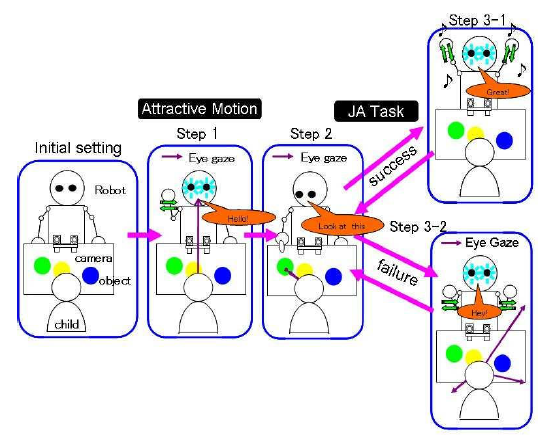
\includegraphics[width=0.6\textwidth]{./img/ravindra2009therapeutic.png}
	\caption{Robot behavior loop used by Ravindra et al. \cite{ravindra2009therapeutic}}
	\label{fig:ravindra2009therapeutic}
\end{figure}

In Diehl et al.'s review, it was pointed out that studies in skill training would benefit from integrating robots into the ABA framework \cite{diehl2012clinical}.  As discussed in Section \ref{sec:DTTDiscussion}, this is what we propose any skill training ATC system should do, similar to COACH.  Thus including a robot into our COACH system would fill this research gap.


In all, from these studies, we see a great potential for increasing the attention and engagement level of the ASD child if we incorporate a humanoid robot into our COACH system.  The robot may serve as an attention grabber as well as a prompting agent.

%%\section{Visual Focus of Attention Estimation}
%Some kind of intro is needed here on why it is important to review the literature in this area.  It doesn't come across anywhere that this is a key technique you are using and why.
One of the key initiators of communication is joint attention, and grabbing and maintaining the visual attention of the user is an important functionality in the design of socially assistive robots \cite{torta2012can}.  In the context of this thesis, a robot is used to teach and practice hand-washing skills with children with ASD.  In its interaction with the child, successfully grabbing and maintaining the child's attention during the activity will ensure the child receives the prompts as the robot delivers it, and thus increasing the chance that the child complies to the prompts.  To this end, the robot behaviors need to be engaging to the child.  But more importantly, the robot behaviors should be contingent to the child's behaviors.  If the child is not paying attention, for example, an attention grabber (e.g. robot waves hand and call out to the child) would serve as a communication opener before delivering the prompt.  This enables the system to adhere to the DTT prompting framework mentioned in \ref{DTTDiscussion}.  Because of this, the robotic system needs to be able to detect the visual attention of the child in real-time.

\subsection{Visual Focus of Attention and Gaze}
If we define Visual Focus of Attention (VFOA) as what a person is looking at, then given that we know what and where objects of interest are in the scene, the problem for VFOA estimation becomes estimating the direction and depth of a person's visual focus (i.e., gaze).
%Are there not standard definitions of these things that you can use and reference?

For consistency, we define the 3 degrees of freedom (DOFs) of head pose as pan, tilt, and roll (see Figure \ref{fig:murphy2009head}), with reference direction for pan and tilt being frontal direction of the head facing the camera.  We define 2 DOFs of eye pose as pan and tilt similar to head pose, with reference direction for pan and tilt same as head pose.
\begin{figure} [h]
	\centering
	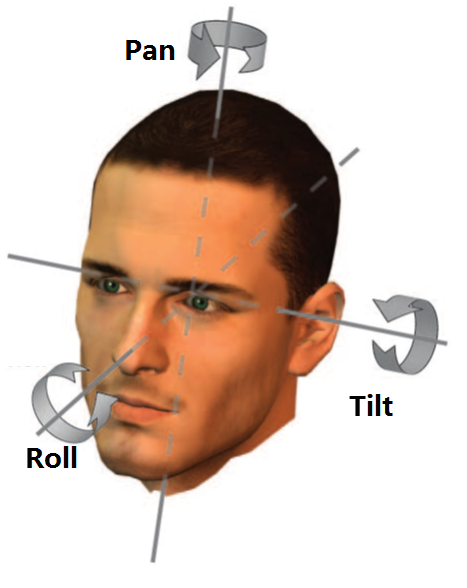
\includegraphics[width=0.6\textwidth]{./img/murphy2009head.png}
	\caption{DOFs of Head Pose, adapted from \cite{murphy2009head}}
	\label{fig:murphy2009head}
\end{figure}


Then, gaze direction is given by the accumulated rotation of average eye pose on head pose \cite{funes2013person}, gaze depth is given by the intersection of the left and right eye pose directions.  Therefore, the problem can be divided into head pose estimation and eye pose estimation.


\subsection{Head Pose Estimation}
There has been extensive research for head pose estimation for a single image frame, or head tracking for a video stream of images.  As reviewed by Murphy-Chutorian et al., the following categories of methods have been identified: appearance templates, detector arrays, nonlinear regression methods, manifold embedding methods, geometric methods, and flexible models \cite{murphy2009head}.


\subsubsection{Appearance Templates and Detector Arrays Methods}
Appearance templates methods and detector arrays methods are mainly for estimating discrete / coarse head pose.  For our task of identifying the object of interest under visual focus of attention, we do not know a priori where and how close to each other the objects are.  Therefore, only continuous fine pose estimation methods are of interest and are reviewed in this thesis.


\subsubsection{Nonlinear Regression Methods}
Using a machine learning approach, a direct mapping from the cropped head image to pose can be learned.  Because such mapping is highly nonlinear, nonlinear regression methods, such as Support Vector Regressors (SVR) \cite{li2000support} and Neural Networks (Multilayer Perceptron (MLP) \cite{voit2008head}, and Locally Linear Map (LLM) \cite{kruger2002gabor} have been applied in this context as supervised learning, using head images as inputs and head poses as ground truths.

Although neural networks are among the most popular and accurate methods in head pose estimation, they are prone to errors from poor head localizations.  And since, in our application, we cannot restrict user to remain in the center of the camera's field of view at all times, we need to either seek out a separate localization method for cropping the head, or seek a head tracker that doesn't have this problem.  Using face detectors for localization is one solution, but it only works for near frontal poses, bottlenecking the head tracker's operating range.


\subsubsection{Manifold Embedding Methods}
Manifold embedding methods learn a projection from high dimensional image space to some low dimensional space.  The methods are unsupervised learning methods that only require head images and not pose ground truth labels.  Promising techniques include: Isometric feature mapping (Isomap) \cite{raytchev2004head}, Locally Linear Embedding (LLE) \cite{roweis2000nonlinear}, and Laplacian Eigenmaps (LE) \cite{belkin2003laplacian}.


However, due to the fact that they ignore pose labels, the projected low dimensional space may not be capturing appearance variations due to head pose alone, but may also include appearance variations due to identity, lighting, etc., making pose prediction inaccurate.  Although there are work around techniques in the manifold embedding methods to tackle the appearance variations due to identity, more systematic ways to deal with it are seen in the following two methods: geometric methods and flexible model methods.


\subsubsection{Geometric Methods}
Geometric methods use person independent facial features (e.g. corners of eyes and mouth, tip of nose, etc.) to predict head pose.  The relative locations of these features are exploited with geometrical assumptions of a person's face such as parallelism, symmetry and proportion \cite{wang2007enhancement}.


A major caveat of these methods is that their accuracy relies on accuracy of features tracking.  For our scenario of a child washing hands at the sink, where a moderate resolution camera captures a mid-range field of view, features are not guaranteed to be tracked with ease.  Thus, it is better to select head pose estimation methods that do not require local features tracking.


\subsubsection{Flexible Model Methods}
Flexible model methods explicitly models the identity as well as pose of a person's face.  Given a representation of the face, flexible models for shape and texture can be constructed using PCA from a face database to represent the directions in which the face most likely (naturally) deforms.  Using this model, a new face image can be fitted through optimizing both an identity parameter and a pose parameter.  This way, pose can be extracted independent of identity.


There are two popular and related flexible model methods: Active Appearance Model (AAM) and 3D Morphable Model (3DMM).  They differ in the following ways:

\paragraph{Face Representation}
Although both models use triangulated mesh representations of the face, AAM uses a 2D representation while 3DMM uses a 3D one.  Also, AAM uses a sparse mesh with vertices at local features while 3DMM uses a dense mesh with vertices at the pixel level.  These make AAM more computationally efficient, but on the other hand 3DMM more robust to low resolution image, partial occlusions, lighting variations, and large head rotations.


\paragraph{Face Fitting}
Because AAM operates in 2D, fitting simultaneously the pose as well as the identity parameters requires us to recover a 3D model of the face using a structure-from-motion algorithm and then use the 3D model's weak perspective projection to constrain 2D fitting \cite{xiao2004real}.  3DMM fitting is less convoluted if using a RGB-D camera (e.g. the Kinect camera).  The pose and identity can be fit simultaneously using a non-rigid iterative closest point algorithm (Optimal Step Non-rigid ICP) \cite{paysan20093d}.

\subsubsection{Kinect Fusion}
Very similar to 3DMM, the Kinect Fusion algorithm developed by Microsoft also can be used to build a 3D head model, and track its orientation through ICP \cite{newcombe2011kinectfusion}.  The main difference between the two algorithms lies in that 3DMM uses the optimal step non-rigid ICP, which uses a parameterized model of a person's face generated by doing PCA of a face model database.  On the other hand, the head model generation from Kinect Fusion simply rely on building a point cloud of the head, thus its model is not parameterized.  Besides this head model generation step that is different, everything else used in head pose tracking are the same -- rigid ICP alignment.  However, since 3DMM focuses on modeling the face while Kinect Fusion is capable of modeling the whole head, Kinect Fusion may perform better in tracking extreme head poses where the face is largely obstructed.  3DMM, on the other hand, can be tolerant of dynamic expressions on a person's face \cite{amberg2008expression}, while Kinect Fusion may yield poorer tracking when the head model deforms.

\subsection{Eye Pose Estimation}
Eye pose estimation for a single image frame, or gaze tracking for video stream of images, have also been extensively researched.  Here we present results from a recent review by Hansen et al. \cite{hansen2010eye}.  Eye pose estimation methods can be categorized as shape-based, feature-based, and appearance-based:


\subsubsection{Shape-Based Methods}
Shape-based methods are seeking to contour fit the shapes of iris, pupil, eye, etc.  Some examples include: a simple model of ellipse fitting the shape of iris or pupil region, proposed by Valenti et al. \cite{valenti2008accurate}; a complex model of deformable template fitting the eye and pupil shape, proposed by Colombo et al. \cite{colombo1999real}.


\subsubsection{Feature-Based Shape Methods}
Feature-based shape methods seek eye structure localization through identifying a set of distinctive local features.  One can use features directly in the intensity image, with features found for example in limbus, pupil, cornea reflections, eye corners, etc.  An example for this is the neural network method by Reinders et al. \cite{reinders1996locating}.  One can also use features in a filter response of the image, for example seen in the method of A Sirohey et al. \cite{sirohey2001eye}.


Both the shape-based and feature-based methods are inaccurate for moderate resolution mid-range field of view images -- they often require a close up view of an eye.  The problem with large field of view containing not only the eye regions is two fold.  First, lower resolution for the eye regions are available, making the above methods less accurate.  Second, without a proper localization of the eyes, false positives arise.  Methods combining head pose and eye pose estimation is an effective way to combat the false positives in a large field of view as well as dealing with large head poses.  It improves accuracy through the two estimators constraining each other in localizations \cite{valenti2012combining}.  However, a better way, as seen in the head pose tracking section of the literature review, is to use appearance-based methods.


\subsubsection{Appearance-Based Methods}
Another approach to deal with moderate resolution mid-field images is through appearance-based methods.  One can directly model the mapping from eye appearance to eye pose, seen by the neural network method of Baluja et al. \cite{baluja1994non}.  However, direct modeling requires large number of training images, the collection of which is a tedious process.  One way to reduce number of training images needed is through template matching with local linear interpolation.  An example of this is the Adaptive Linear Regression (ALR) method of Lu et al. \cite{lu2011inferring}.


The major caveat with these appearance-based methods, as similarly to head pose estimation, is the inability to separate appearance variations in identity from pose.  One way to tackle this is through keeping a bank of personal models, seen in Mora et al. \cite{funes2013person}.  A new person's eye images can then be represented by a linear combination of exemplar eye images from people in the bank using ALR.  Then, to ease computational cost of ALR, we only keep the top few models that have their exemplar eye images used most often, decreasing the search space during ALR's optimization step.


\subsection{Using RGB-D Camera for Gaze Estimation}
The works of Mora et al. are good fits to our application \cite{funes2012gaze, funes2013person}.  Specifically, their approach uses the 3DMM head pose estimation together with ALR eye pose estimation.  One thing to note is that the commercial grade RGB-D camera, Kinect, is used.  Although 3DMM works with 2D camera as well, getting a direct sensor input on the depth information is advantageous in this context because it avoids inferring the 3D structure from 2D images, reducing inaccuracies and computations. Also, it enables 3DMM to estimate pose through shape alone, ignoring texture fitting altogether, reducing computations and increasing robustness to lighting.


\subsection{Discussion}
From the reviews, we see that Kinect Fusion and ALR are ideal for our application.  They yield many advantages:  Firstly, usage of appearance-based methods means we are moderate resolution mid-field scenario ready.  Secondly, only a simple calibration step is needed to generate the head model for Kinect Fusion and a bank of people's exemplar eye images are needed for ALR.  For the children with ASD population, having relatively simple calibration step that does not require the child to behave in a certain way is very useful.  Next, once the person's head model is generated, pose can be fitted without fitting identity, reducing computations.  Lastly, the head image can be restored to the frontal head pose and a consistent frontal eye region cropped out, making eye pose estimation robust to large head poses.



\chapter{Research Objectives}

\section{Overall Goal and Approach}
Our overall goal is to increase a child with ASD's engagement level during COACH prompting and task execution, and thus improving prompt compliance and task completion rate.  Our approach is:
\begin{enumerate}
	\item to incorporate a half body humanoid robot, NAO T14 (see Figure \ref{fig:HalfBodyNAO}) by Aldebaran Robotics, into the current COACH setup, capable of delivering verbal and gesture prompts and attention grabbers.
	
	\item to automatically track the VFOA of child for more effective maintenance of child's attention.  For example, by being able to recognize whether child is looking at the robot, the robot can call out child's name with a waving gesture or blink its LEDs for getting child's attention before prompting.
	
\end{enumerate}
\begin{figure} [h]
	\centering
	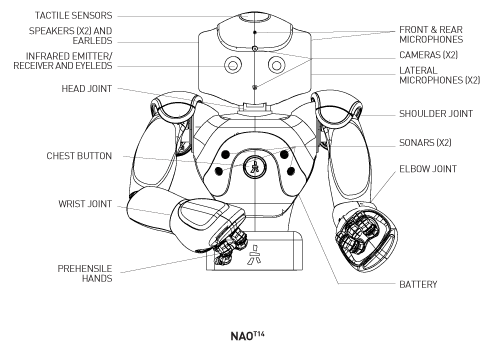
\includegraphics[width=0.6\textwidth]{./img/nao_t14_schema}
	\caption{The Half-Body Version of Humanoid Robot NAO}
	\label{fig:HalfBodyNAO}
\end{figure}


\section{Central Hypothesis}
We hypothesize that the incorporation of a humanoid robot prompting agent, such as NAO T14, would sufficiently capture and maintain children with ASD's attention during prompting and keep them engaged during task execution, so that high prompt compliance rates and task completion rates would be achieved when assisting them through ADLs such as hand-washing.


\section{Specific Objectives}

\paragraph{Our objectives are:}
\begin{enumerate}
	\item To investigate if a prompting system using NAO is able to guide child with ASD through hand-washing.
	
	\item To explore the different modes of interactions between NAO and child when prompting hand-washing steps using a Wizard of Oz setup, focusing on verbal, gestures, and gaze for the modes of interactions
	
	\item To implement a real-time algorithm for tracking child's VFOA
\end{enumerate}



\paragraph{Our hypotheses are:}

%	\item Child has greater general engagement level when interacting with NAO than with the parent.


%general engagement level:
%# of times child smiles
%# of times child murmurs
%# of times distracted

%visual focus correct:
%look at prompting agent given prompt rate
%look at step attempted given attempt rate

%prompt compliance and task completion:
%compliance rate
%# of prompts till compliance
%time duration till compliance
%task completion rate
%# of prompts till finished step before prompt
%time duration of extended steps
%number of presses for soap
%# of times requiring physical intervention

%independence:
%# of times child start step before prompt
%# of times child finishes step before prompt

%what measures for survey? just qualitative report? any processing / analysis needed before reporting?

\begin{enumerate}
	\item The humanoid robot, NAO, is able to independently assist child with ASD through hand-washing, and child exhibits greater engagement level, higher prompt compliance rate, and better task completion when prompted by NAO than by parent.
	
	\item Gestural, gaze, and verbal are the essential modes of interactions present in the hand-washing prompting scenario between child with ASD and the prompting agent NAO.
	
	\item Using 3DMM and ALR for estimating head pose and eye pose, and using the Kinect camera, a classification rate of more than 80\% is achieved for estimating child's VFOA on NAO, monitor screen, soap, towel, tap region, hands, and idling.
	
\end{enumerate}

\chapter{Wizard of Oz}

%What are we trying to find out? Why are they important?
%	- is there a difference in child's response to parent prompt vs robot prompt?
%		- visual attention
%		- compliance
%		- task performance

One major objective of this thesis is to investigate the impacts that using a humanoid prompting agent has on the visual attention, prompt compliance, and task performance of children with ASD during hand-washing activities.

This is the first research of its kind in the field of humanoid robot prompting agent guiding children with ASD through an activity of daily living.  Therefore, it is wise to begin with a pilot study, the purpose of which is to show plausibility of the key underlying assumptions of our hypotheses, and to probe what questions are important to be answered later in a more rigorous randomized control trial.  For this reason, the pilot study should be exploratory in nature, having a flexible experiment design, and relatively low experiment setup cost.

%WoZ experiment design
%	- what is WoZ? why do we use this scheme?
%	- experiment design, why use this design
%	- short blurb of the experiment
%Recruitment
%	- inclusion criteria
%	- method of recruitment, target sample size
%NAO
%	- overall description, capabilities
%	- general design decisions for
%		- verbal prompts
%		- gesture prompts
%Protocol and Setup
%	- experiment / equipment setup for data collection
%	- protocol
%	- video data to be collected
%	- survey to be collected
%	- ethics considerations
%Video annotation protocol
%Measures
%Analysis and results:
%	- participants recruited
%	- video data collected
%	- video analysis method
%	- video analysis results
%	- inter-rater agreement analysis and results
%	- survey data collected
%	- survey analysis method and results
%Discussion:
%	- results interpretations
%	- interpretation limitations
%	- original objectives achieved or not
%	- future outlook

\section{Wizard of Oz Experiment Design}

The Wizard of Oz (WoZ) is an experiment design widely used in Human Computer Interaction (HCI) and Human Robot Interaction (HRI) research.  In a typical WoZ study, there is an interactive agent that is not yet fully autonomous, and is remotely controlled by a human operator (i.e. the "wizard"), and this fact is concealed from the user being tested until after the study.  The wizard may control one or many parts of the agent, such as speech recognition and understanding, affect recognition, dialog management, utterance and gesture generation and so on \cite{bhargava2013demonstration}.  The advantage of a WoZ study is that it does not require a large amount of work spent in implementing the artificial intelligence (AI) behind the agent before testing it in a study -- it is mocked up by the wizard remote controlling the agent.  This is great for testing hypotheses early on in the design loop, enabling us to obtain feedbacks from users, learn, and iterate through design cycles faster.  Of course, care needs to be taken to ensure the mocked up part of the AI is implementable in the near future, since the real purpose of the mock up is to have an early knowledge of the real design constraints, not trying to provide a less constrained solution.

The characteristics of a WoZ study fits our pilot study requirements, where we want to learn early the important design questions regarding building an effective ADL prompting robotic agent for the children with ASD population.  Thus, we have conducted a WoZ study in which a humanoid robot whose motions and speech were preprogrammed, but the decision and timing of their executions were controlled remotely by the researcher.  The researcher, acting as the wizard, is mocking up the computer vision algorithms that understand the child with ASD's actions, the speech recognition algorithms that recognize the child's verbal interactions, and the AI decision making algorithms that decide what prompts to deliver and when to deliver them.

During each WoZ study trial, the child with ASD would be asked to complete the hand-washing activity in the washroom with the supervision of one of his/her parents, with the help of the NAO robot, or with the help of both the parent and the robot. The researcher, and the parent if the child was to be assisted only by the robot, would be in an adjacent room out of the child's view to observe his/her hand-washing activity.  However, the parent could enter the washroom if the child needs physical assistance to complete a step. A controlling interface running on a laptop, connected wireless to the robot, was used by the researcher to remotely control the robot, as well as to monitor the progress and responses of the child through the video feeds of the cameras installed in the washroom.


\section{Recruitment}
\label{sec:Recruitment}
Since children with ASD are a diverse population with each child unique and vastly different from another, the subpopulation from which we recruit from directly influences our study results and focus.  This is the process of case selection.  Since the aim of our study is to test feasibility of our approach, and form important hypotheses about HRI with children with ASD that aid in future iterations of the robot prompting design, focusing on the typical use case would be most beneficial at the pilot study stage.  One way to ensure this is through sampling for the typical user that our robot is designed for.  This would be children with ASD, not adults nor any one without a diagnosis of ASD.  In addition, the participant needs to be able to interact with a prompting agent, understanding and following its instructions.  Gender, ethnicity, and other factors that are not significant in determining important robot design recommendations are not constrained in our inclusion criteria.  In addition, hand-washing skills are constrained to a certain degree, but the level of hand-washing skills need not be non-existent.  All participants yield valuable design input information as long as the participant requires some form of assistance during hand-washing, whether it be requiring prompts to get started, to know which steps to execute, or to know how to execute each step.  This means, on the spectrum of hand-washing levels, we might have several different cases depending on the participants we recruited.

Participants were recruited from a list of families of a previous autism study that indicated that they would be interested in participating in future studies related to the development of the COACH prompting system.  The inclusion criteria for enrolling in the study were as follows:
\begin{itemize}
	\item Boys and girls between the ages of 4-15 years
	\item Parent report of a clinical diagnosis of an ASD – to be confirmed through administration of the Social Responsiveness Scale (SRS)
	\item Has difficulty independently completing self-care activities, specifically hand-washing
	\item Has the ability to follow simple, one-step verbal instructions
	\item Ethical consent  granted by parents or primary guardian
	\item Does not exhibit severely aggressive behavior
\end{itemize}
Three children would be recruited. This sample size is typical for studies of this nature (i.e. HRI case study for children with ASD), e.g. Kozima et al. had two participants in
\cite{kozima2005interactive}, Robins et al. had three in \cite{robins2004robot} and \cite{robins2009isolation}.  Participant demographics, namely age, sex, and the Social Responsiveness Scale (SRS) test results, were recorded.  The SRS is a commonly used tool to identify the presence and estimate the severity of ASD \cite{constantino2002social}. Reporting the results of the SRS would allow a better understanding our research results in context of the participant's conditions.

Each participating family was given a \$200 honorarium per child subject upon completion of the study. All participants were able to withdraw from the study at any time. The honorarium would then be adjusted to be proportionate to the number of visits completed (e.g. completing 3 visits means the participated child would receive \$100 (\$200 * 3 / 6 = \$100)). This would be made clear to participants at the time of consent.
\section{Humanoid Robot NAO}

We chose the torso and arms only version (T14) of the commercially available humanoid robot NAO from Aldebaran Robotics as our robotic prompting agent.  NAO is a humanoid robot about half a meter high in torso (see Figure \ref{fig:NAOColor}).  It is designed by Aldebaran Robotics to primarily serve academic research in robotics.  NAO is equipped with the state of the art mechanical, electrical, embedded, control, and local network communication systems.  It also has cameras and sonar sensors for computer vision algorithms for scene understanding, path planning, and obstacle avoidance.  The software development kit (SDK) provided is very easy and powerful to program with.  Also, an even easier graphic user interface (GUI) for robot behavior programming, the Choreographe software, is also available.  One caveat of using NAO for SAR HRI research is that it is only equipped with a single degree of freedom finger dexterity, though other joints in its body are much more mobile.  It is more than enough for doing simple pointing and other non-contact gestural prompts in sync with verbal interactions.  It just cannot perform detailed hand gesturing.  This makes NAO less capable in demonstrating a hand-washing step in high detail.
\begin{figure} [h]
	\centering
	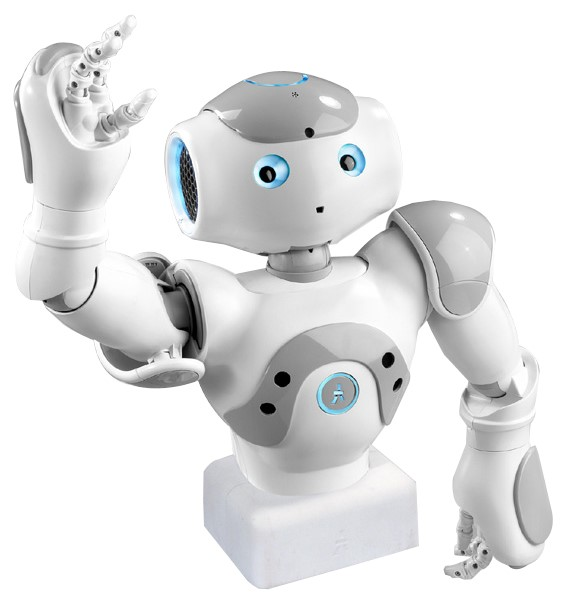
\includegraphics[width=0.6\textwidth]{./img/nao-torso.jpg}
	\caption{NAO T14 Humanoid Torso}
	\label{fig:NAOColor}
\end{figure}


From a HRI research perspective, Aldebaran Robotics took care of designing the intrinsics level of HRI, where NAO has a likable appearance and child like neutral gender voice, although it is incapable of facial expressions.  The design decisions we face when using NAO for this thesis is on the behavior level of HRI.  Design decisions such as voice intonation choice, verbal prompts, motion gestures and gaze, and eye blinks using LEDs in eye regions are made in this thesis.  The objective of this thesis is then to ultimately find out if the lower two levels of design decisions made are able to cumulate to the child with ASD perceiving NAO as a role model / supervisor / assistant during hand-washing.

For our pilot study, we use the half-torso version of NAO because we do not require any mobility from NAO -- it is fixed on the sink table top (see Figure \ref{fig:ExpSetup}).  The relevant functionalities of NAO we utilized for delivering prompts include:
\begin{itemize}
	\item Verbal prompting through its bilateral loud speakers on the head and speech synthesis functionality
	\item Body gesturing through its moving head and arms (although its fingers are not capable of hand gesturing)
	\item Flashing LEDs on the eyes and ears
\end{itemize}
\begin{figure} [h]
	\centering
	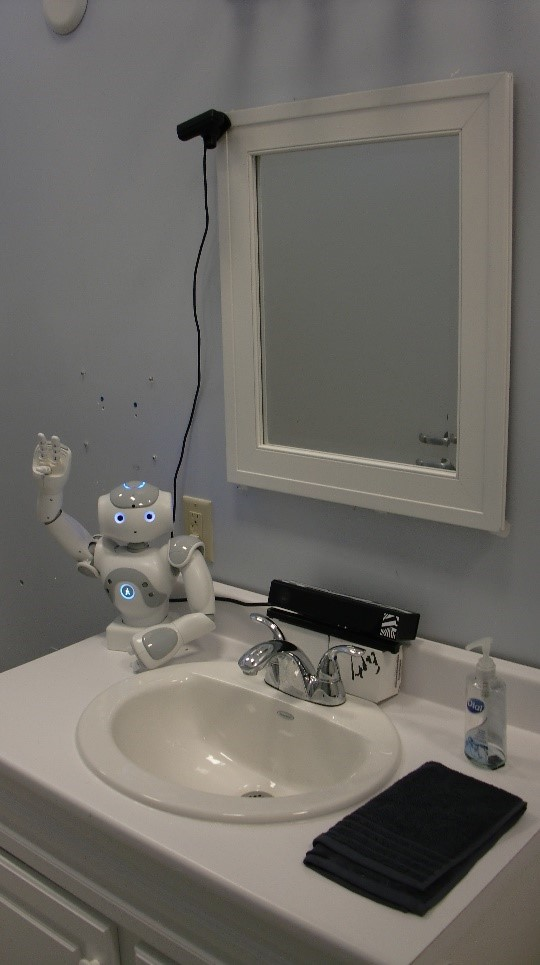
\includegraphics[height=15cm, keepaspectratio]{./img/exp_setup.jpg}
	\caption{Experiment Setup}
	\label{fig:ExpSetup}
\end{figure}


\subsection{Verbal Prompts}
We used the text-to-speech engine from NAO to synthesize the verbal prompts.  The pitch of NAO's voice was changed to a lower one than default for the verbal prompts to give a more authoritative feeling.  The reward verbal prompt remained the default pitch, though, to give an exciting praise.  The verbal prompts were worded as short, three or four words phrases, such as "turn on the water" or "rinse your hand", and a pause is put between the action and the subject so that the prompts sounded clearer and was easier to understand to children with ASD.  The specific choices of verbal and gesture prompts are discussed in Section \ref{sec:SpecificProtocol}.

\subsection{Gesture Prompts}
There are several kinds of gesture prompts NAO needs to perform:

\begin{itemize}
	\item \textbf{Attention grabber (AG)}:  When prompting is needed but the child is not looking at NAO, NAO waves to grab the child’s attention.
	\item \textbf{Motion demonstrating prompt (MoDemo)}:  NAO demonstrates to child the motion of interaction (e.g. turning tap, scrubbing, rinsing, etc.).
	\item \textbf{Object pointing prompt (ObjPt)}:  NAO points to the physical object of interaction.
	\item \textbf{Reward (REW)}:  After a task is successfully completed, NAO flashes LEDs as a positive reinforcement.
\end{itemize}

The gaze behaviour of NAO during gesture prompts is also important and is grouped as: looking at child (when delivering AG, MoDemo, REW), and looking at object (AR, ObjPt).  The gesture and gaze motions can be programmed using NAO's software, Choregraphe.

\subsection{Wizard of Oz Remote Control}
The WoZ experiment setup involves controlling the robot remotely behind the scene by a human operator, the wizard.  A touch screen laptop was used as the user interface for the operator, and the behaviors of the robot were presented as buttons on the screen, with the camera views displayed along side.  Keyboard shortcuts were also implemented for faster access to robot actions.

\section{Surveys}
In addition to observing the child with ASD interacting with the robot, surveys were designed to probe the child's background, experiences, and preferences, putting the observations into context.  Also, surveys probing the parent's opinion of the robot and the COACH system were also created, since the parent is also an important decision maker in the robot and the COACH system's design.

\paragraph{Social Responsiveness Scale Survey and Entrance Survey}
The Social Responsiveness Scale Survey serves to screen participants during recruitment and was filled out by the parent that accompanied the child to all trials.  The entrance survey was administered along with the SRS survey.  It reports the child's demographics as well as inclusion criteria fit.  In addition, it also reports child's previous experiences with technologies, child's personal preferences, child's abilities on hand-washing and on other ADLs, and parent's expectation and concerns.

\paragraph{Post-Intervention Survey}
During the last visit, the same parent who completed the SRS survey and the entrance survey was be asked to fill out the post-intervention survey.  The survey reports the parent's opinion on the robot prompting system, giving suggestions and comments and how effectiveness and appropriate the system is, and any improvements or adjustments needed.

\section{Study Protocol and Setup}
\label{sec:StudyProtocol}

%protocol:
\subsection{Conducting Entrance and SRS Surveys}
Prior to their first visit to the lab, the parent was asked to complete the Social Responsiveness Scale (SRS). If the child met the SRS score (minimum of 76 T-score), the same parent would then be asked to complete the entrance survey before their first visit. This same parent was required to accompany the child through all visits.


\subsection{Hand-Washing Trials Protocol Overview}
\label{sec:ProtocolOverview}
The trials were carried out in the washroom inside the HomeLab -- a laboratory specifically designed to emulate the home settings, located on the 12th floor of Toronto Rehab Institute (more details of the experimental environment is described in Section \ref{Sec:ExpSetup}).  Each child would visit the HomeLab once a week with a total of six visits with his/her parent. The six visits would consist of three kinds of phases. The three phases are namely the baseline phase (Phase A) and the intervention phases (Phase B and Phase C). In Phase A, the child would be asked to wash hands by him/herself as independently as possible. The parent was instructed to provide assistance to the child as the parent saw necessary.  In Phase B, the child would be assisted by the robot NAO alone.  The parent was out of view in the room adjacent to the washroom, and came into the washroom to guide the child to continue if the child got stuck or finished early and was leaving the washroom.  In Phase C, the child would be assisted by NAO and the parent together.  The parent remained in the washroom and assisted robot NAO in its prompts.  Phase C had the purpose of the parent showing the child how to follow the robot as the robot prompts the child.  The parent was left to his/her best judgment in how to work together with the robot.

Each visit took about an hour to an hour and a half. The child was asked to wash his/her hands eight times for every visit, for a total of forty-eight trials per child.  This way, the consecutive trials conducted within a day would hopefully be not too much for the child to cause fatigue.  The child and his/her parent could take short breaks after each hand-washing trial.  The break could last as long as the child needed until he/she was willing to continue the trial. If the parent felt the need, they could leave and come back to finish the rest of the day's trials another day. They would not be withdrawn from the study unless requested.

We conducted the phases in the order A-B1-C-B2 (i.e. parent alone phase - robot alone phase - robot parent phase - 2nd robot alone phase).  By splitting the phase B to Phase B1 and Phase B2 and flanking phase C, we can compare Phase B1 and Phase B2 to see how much did learning in Phase C affect our results.  We aimed to approximately have sixteen trials per phase, which gives a good sample size for both quantitative and qualitative analyses.  This means Phase B1 and Phase B2 would have about eight trials each.  Note that the number of trials for each phase might be adjusted by the researcher depending on the ongoing data analysis, and the parent researcher interviews would be used as the basis for such adjustments.  More detail on how to adjust is discussed in Section \ref{sec:ConductingInterviews} - Conducting Interviews and the Basis of Sample Selection.  The actual number of trials conducted for each phase are reported in Section \ref{sec:CaseSamplesSelected} - Case and Samples Selected.


\subsection{Experiment Setup}
\label{Sec:ExpSetup}
The equipment was set up near the sink, which included a NAO robot, an overhead camera, a scene camera, and a Kinect camera. The NAO robot is a small half-torso humanoid robot and was screw-mounted on the sink countertop at the top left corner (please see Figure \ref{fig:ExpSetup}). The NAO robot delivered verbal and gesture prompts to the children with ASD while they were performing the hand-washing tasks.  The overhead camera was installed on the wall/mirror right above the sink. The overhead camera recorded objects on the sink countertop (e.g., taps, faucet, soap, and towel). The purpose of the overhead camera was to capture the hand actions of the child during hand-washing in order to track the child's progress along the tasks. The scene camera was placed on the floor on a camera stand with its field of view including all objects in the scene (e.g., robot, child, and objects on sink countertop). The purpose of the scene camera was to capture the child's engagement and attention during the prompts as well as during task executions. The Kinect camera was mounted on the sink countertop underneath the mirror and behind the tap. The Kinect camera recorded mainly the child's face. The purpose of the Kinect camera was to capture the child's face during hand-washing for the development of an automatic algorithm that estimates the child's gaze direction in real-time. Examples of the images captured by the three cameras are shown in Figure \ref{fig:CameraViews}.
\begin{figure}[H]
	\centering
	\begin{subfigure}[b]{0.49\textwidth}
		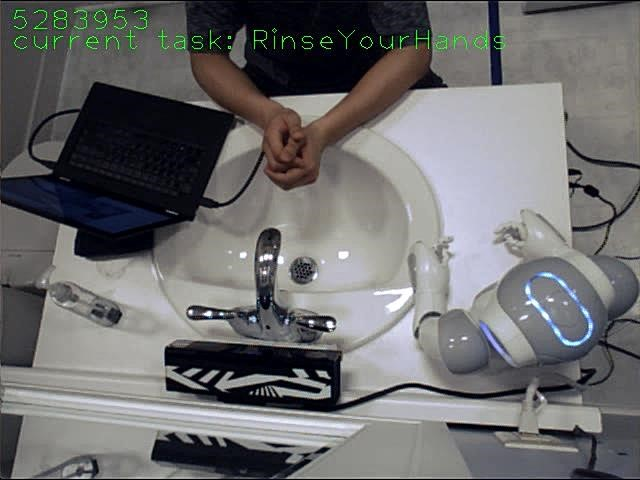
\includegraphics[width=1.1\linewidth]{./img/overhead_view.jpg}
		\caption{Overhead Camera View}
%		\label{fig:7TotalNumberofIncompleteSteps-BeforeParentorRobotPrompts}
	\end{subfigure}
	
	
	\begin{subfigure}[b]{0.49\textwidth}
		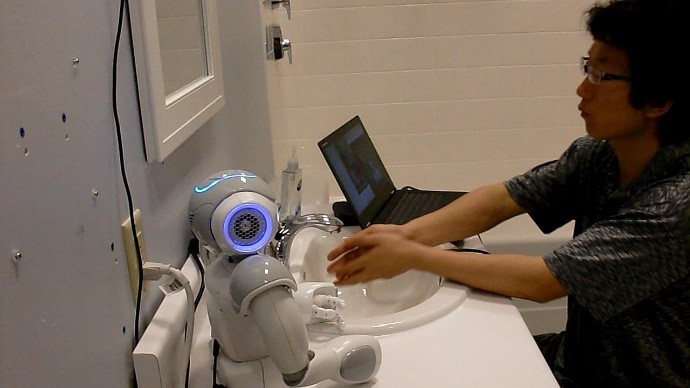
\includegraphics[width=1.1\linewidth]{./img/scene_view.jpg}
		\caption{Scene Camera View}
%		\label{fig:6TotalNumberofIncompleteSteps-BeforeParentPrompts}
	\end{subfigure}%
	
	
	\begin{subfigure}[b]{0.49\textwidth}
		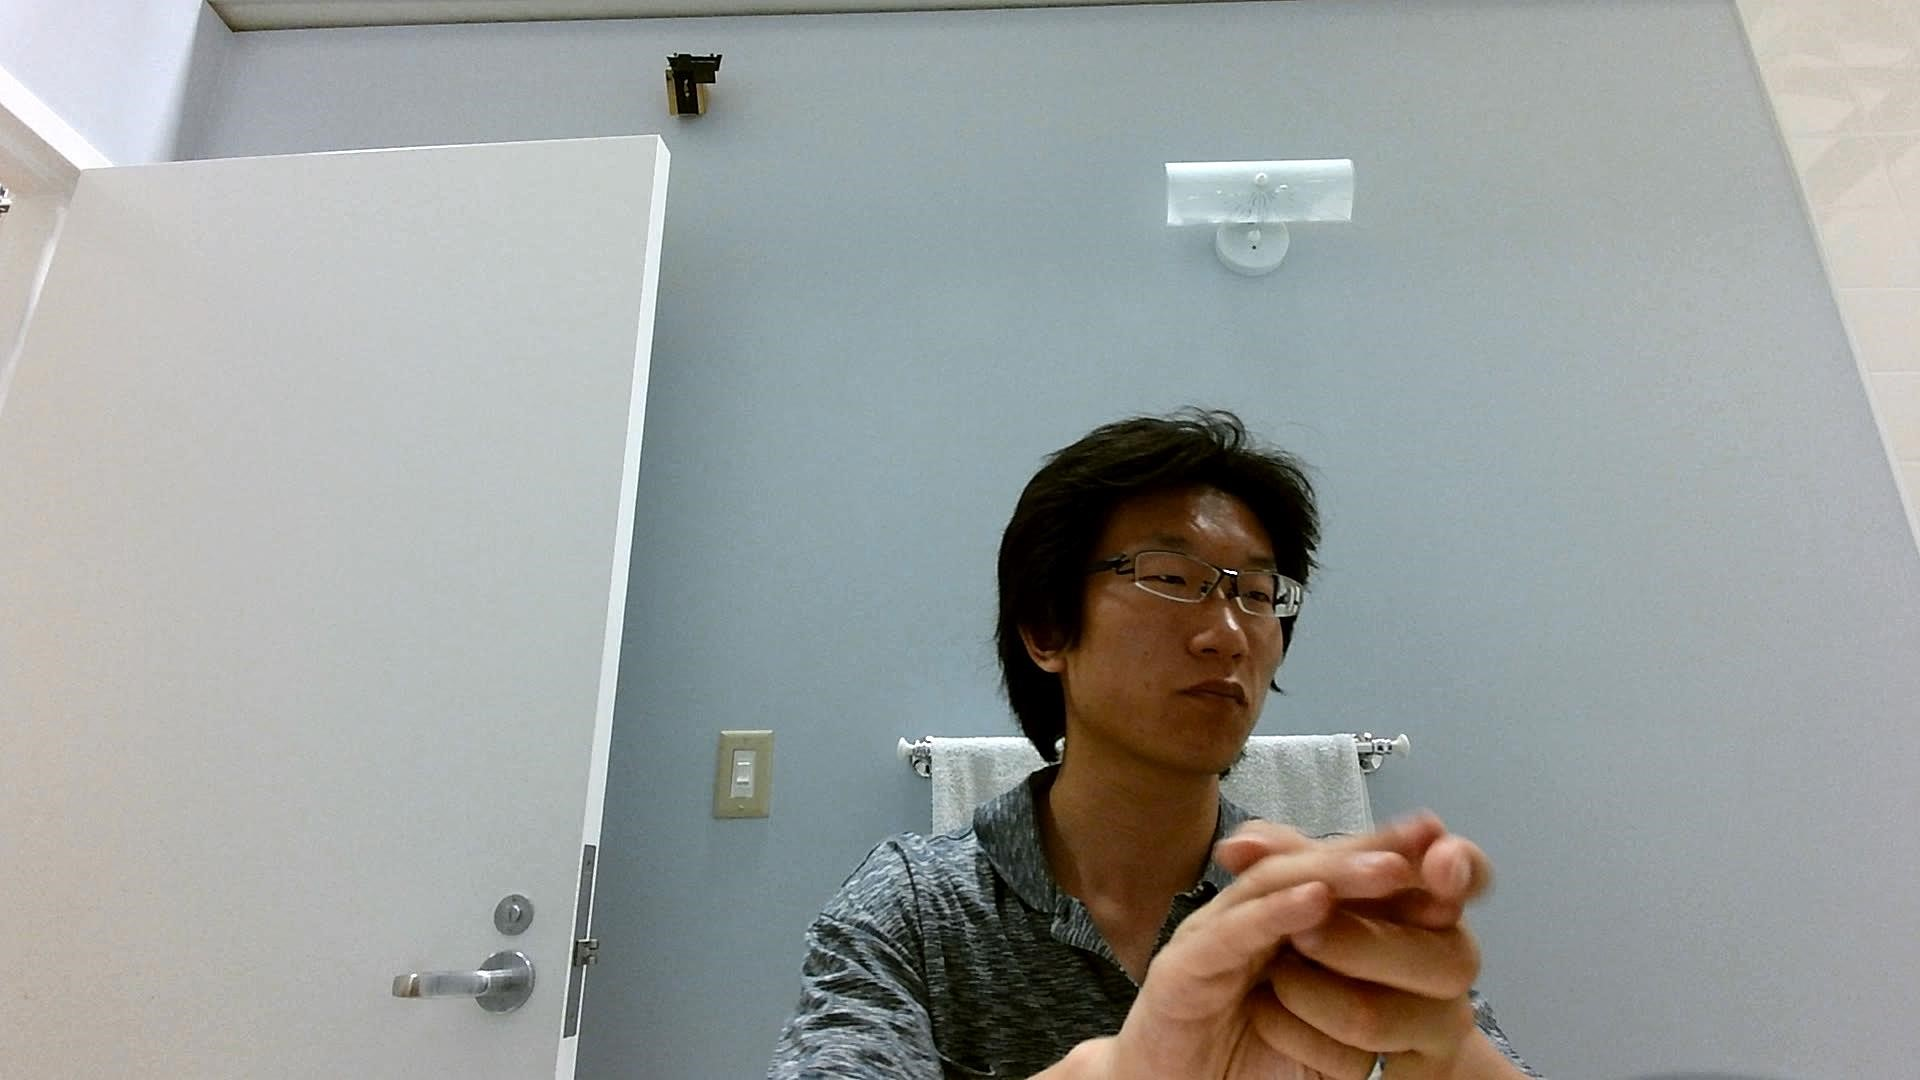
\includegraphics[width=1.1\linewidth]{./img/kinect_view}
		\caption{Kinect Camera View}
%		\label{fig:5TotalNumberofIncompleteSteps-BeforePhyiscalPrompts}
	\end{subfigure}%
	
	\caption{The views of the three cameras used in the WoZ study.}
	\label{fig:CameraViews}
\end{figure}


A touchscreen laptop was used during the study by the student researcher to control the robot. It connected to the robot wirelessly. The laptop also connected to the overhead and Kinect cameras through USB cables to provide real-time video feed. The data collected from the cameras was saved temporarily in the laptop hard-drive.

\subsection{Specific Protocol}
\label{sec:SpecificProtocol}
The hand-washing activity was broken down into seven steps: turn on the water, wet your hands, get some soap, scrub your hands, rinse your hands, turn off the water, and dry your hands.  These steps were modified based on Bimbrahw et al.'s pilot study \cite{bimbrahw2012investigating}. These constituted the same steps as Bimbrahw's except that the first (i.e. turn on the water and wet your hands) and the last step (i.e. turn off the water and dry your hands) are now four individual steps to ensure that each step only involved one action.

\paragraph{Phase A (Baseline Phase)}
In the baseline phase, the child was asked to complete the hand-washing as independently as possible. During this phase, the parent was present in the washroom while the child was completing the hand-washing steps. The parent would verbally prompt and/or physically assist the child and give positive reinforcements to the child whenever the parent feels necessary.  Minimal restrictions or guidances were presented to the parent by the researcher, so that what the parent thought were important could become apparent to the researcher.

\paragraph{Phase B1 and B2 (Robot Only Intervention Phases)}
In the robot only phases, the child was asked to wash his/her hands with the help of the robot NAO alone in the washroom. During every trial, NAO waited for the child to start each step. If the child experienced troubles, an appropriate prompt was delivered from NAO in order to help the child complete the step. If the child did not respond to NAO's prompt, an attention grabber was delivered to capture the child's attention to the prompting agent. The attention grabber could be repeated for a second time if the child failed to respond to the first one.  After successfully grabbing the child's attention, the prompt was repeated.  A verbal reward was delivered to the child when he/she completed a step.  The parent was out of view of the child during Phase B1 and B2, and only coming into the washroom to prompt when the child has ignored the robot's repeated attempt to prompt.  The purpose of the parent coming in was first to remind the child to listen to the robot, and only physically help the child to complete the step as a last resort if the child continue to ignore the robot and the parent's prompts.  After the physical intervention in phase B, the parent then instructed and encouraged the child to continue the rest of the hand-washing steps on his/her own by following the robot.


\paragraph{Phase C (Robot Parent Joint Intervention Phase)}
In the Robot Parent Joint Phase, the child was asked to wash his/her hands with the help of the robot NAO and the parent together.  In this phase, the robot behaved similar to that in Phase B1 and B2.  The parent, on the other hand, took a more active role in phase C.  Instead of hiding out of sight from the child, the parent in this phase stood beside the child and told the child what to do.  At the beginning of each trial in this phase, the parent and the researcher chose the amount of involvement the parent had during the trial, whether to prompt the child to listen to the robot as it prompts the steps, to prompt the steps him/herself, or to physically guide the child through the steps.  Of course, for both phases, if the child did not respond to any of the prompts, the parent was to physically intervene and complete the step together, similar to phase A.

Both phases B and C are important.  Phase B1 and B2 serve to test if NAO can independently assist the child through hand-washing with minimal parent involvement.  Phase C serves to investigate if  and how the parent is able to train the child to better follow the robot prompts.  Comparing phase B and C and comparing phase B and A could potentially yield areas of improvements for NAO.

The NAO robot's prompts can be categorized into three groups (please see Table \ref{tab:RobotPrompts} for the specifics of each prompt used):
\begin{enumerate}
	\item \textbf{Step Prompt} (to prompt the child through a hand-washing step):
	
	A verbal prompt is delivered, such as “Please [step name]” (e.g. “Please turn on the water.”).  Synchronous to the verbal, a visual prompt is also be delivered. This is a two-part gesture prompt of: first, demonstrating the motion of interaction while looking at the child (i.e. MoDemo); second, pointing to the sink object (e.g. the tap) while looking at the object (i.e. ObjPt). A maximum of two prompts is given to the child. If the child does not respond to the second prompt or has started the step but does not complete the step within the a reasonable time, the parent is asked to help the child complete the step. 
	
	\item \textbf{Attention Grabber} (to capture the child's attention to the NAO robot): 
	
	A verbal prompt is delivered, such as “Hi, [child's name]!”  Synchronous to the verbal, a visual prompt is also delivered. This is an attention grabbing gesture of waving and looking at the child (i.e. AG). A maximum of two attention grabbers is given to the child in order to get his/her attention to look at the robot.  The parent is asked to instruct the child to look at the robot if he/she does not respond to the second attention grabber. 
	
	\item \textbf{Reward} (to provide positive reinforcement when the child attempts a step without the help from his/her parent): 
	
	A verbal reward (i.e. “Great!”) is delivered while looking at the child and switching back and forth the colors of the light-emitting diodes (LEDs) on the eyes after successfully performing a step (i.e. REW).
\end{enumerate}
\begin{table}[h]
	\centering
	\begin{tabular}{ |l| p{4cm} | p{8cm} | }
		\hline
			&	\textbf{Verbal Prompt}	&	\textbf{Robot Gestures}	\\	\hline
			
		\textbf{Attention Grabber}	&	Hi, [child's name]!	&	Waving and looking at the child.	\\	\hline
		
		\multirow{7}{*}{\textbf{Task Prompts}}	&	Turn on the water!	&	Turning right wrist clockwise while looking at the child, then pointing and looking at the tap.	\\	\cline{2-3}
		&	Wet your hands.	&	Holding out hands while looking at the child, then pointing and looking at the running water.	\\	\cline{2-3}
		&	Get some soap.	&	Pressing down right hand with left hand collecting from below while looking at the child, then pointing and looking at the soap.	\\	\cline{2-3}
		&	Scrub your hands.	&	Scrubbing both hands while looking at the child, then pointing and looking at the child's hands.	\\	\cline{2-3}
		&	Rinse your hands.	&	Holding out hands while looking at the child, then pointing and looking at the running water.	\\	\cline{2-3}
		&	Turn off the water.	&	Turning right wrist counterclockwise while looking at the child, then pointing and looking at the tap.	\\	\cline{2-3}
		&	Dry your hands.	&	Wiping one hand against the other while looking at the child, then pointing and looking at the towel.	\\	\hline
		
		\textbf{Reward}	&	Great!	&	No gestures. Flashing multicolor LEDs on the eyes while looking at the child.	\\	\hline
		
		\textbf{Intro}	&	Hi, [child's name]! Let's start washing hands.	&	Giving an attention grabber gesture followed by a simple conversational gesture while looking at the child.	\\	\hline
		
		\textbf{Re-intro}	&	Let's continue washing hands.	&	Giving a simple conversational gesture while looking at the child.	\\	\hline
		
		\textbf{Outro}	&	Good job, [child's name]! You are all done.	&	Fist pumping in the air, followed by an all done gesture. Flashing multicolor LEDs on the eyes while looking at the child.	\\	\hline
	\end{tabular}
\caption{The Robot Prompts -- Detailed Descriptions.}
\label{tab:RobotPrompts}
\end{table}

For each trial, in addition to the three prompt categories stated above, the NAO robot also delivered a short introduction before the start of each trial, a re-intro after the parent finished assisting the child through a step, and an outro at the end of each trial. The introduction was a two-part prompt. The first part was an attention grabber. The second part consisted of a verbal prompt (i.e. “Let's start washing hands.”) with a simple conversational gesture. The re-intro was a verbal prompt (i.e. “Let's continue washing hands.”) with a simple conversational gesture. Same as the introduction, the outro was a two-part prompt. The first part consisted of a verbal prompt (i.e. “Good job, [child's name]!”) with a gesture of fist pumping in the air. The second part consisted of a verbal prompt (i.e. “You are all done.”) with a gesture signifying all the hand-washing steps have been done.

\subsection{Conducting Interviews and the Basis of Sample Selection}
\label{sec:ConductingInterviews}
The interviews with the parent were conducted by the researcher during every break between trials.  This was to discuss what happened in the last trial, why the child behaved this way, whether we needed to change the robot prompts for improving effectiveness, whether to change the protocol to focus on certain aspects of the study more, and how many more trials of the current phase should we do.  Also, the researcher sometimes requested certain ways the parent was to assist and guide the child, so to explore the influence of the parent on child's interaction with the robot.  Although conducted in an informal conversational format, this interviewing, discussion, and reflection process was a form of qualitative analysis similar to that of making observational field notes.  Thus, the results of these discussions were then used as basis for sample selection, revising the robot behavior and study protocol for the subsequent trials.  This process was continued iteratively, which modeled after the theoretical sampling method defined in Section \ref{sec:CaseSelectionAndSampleSelection}.  Within the theoretical sampling approach, we adopted the maximum variation sampling method by varying the degree of the parent's involvement.

\subsection{Conducting Post-intervention Surveys}
During the last visit, the parent who completed the entrance survey was asked to fill out the post-intervention survey.

\subsection{Data Collection}
All trials were video recorded by the overhead, the scene, and the Kinect cameras and audio recorded by the microphone from the scene camera.  The overhead and scene video data were reviewed and annotated by a single annotator -- the researcher. The overhead video data was used to score the participants' prompt compliance and hand-washing performance. The scene video data were used to evaluate the participants' engagement during the whole activity. Possible areas of improvement of robot prompting will be explored, based on its observed effects on engagement, compliance, and performance.

The Kinect video data was not annotated. Instead, it was collected to be potentially used to evaluate the automatic gaze estimation algorithm that we may develop. Specifically, the Kinect video data could be used as inputs to train a gaze estimation algorithm and the outputted predictions of the algorithm can be compared with annotations of the scene video data to evaluate the algorithm's prediction accuracy.


\subsection{Ethics}
The WoZ pilot study was approved by the Research Ethics Board (REB) of University Health Network (UHN), belonging to which is the Toronto Rehab Hospital, where the study was conducted.

\paragraph{Consent and Assent}
Participants were given a package of consent/assent forms prior to starting the study. One of the parents provided their consent for their child and themselves to participate in the study. In addition, child participants provided their assent to participate in their every visit of the study. 

Interested families received an information/consent package prior to starting of the study. This package includes consent/assent forms for participation in the study for the parent and child with ASD (these forms include study details and research contact information) as well as consent to be videotaped for the parent and child with ASD. Consent from the parent and assent from the child with ASD were given if and when they feel comfortable that they understand the information presented. Potential participants of both parents and children had up to a week to decide if they would like to participate, although they may consent to participate as soon as they feel comfortable doing so. Parents needed to provide their consent for their children and themselves to participate in the study. In addition, child participants needed to provide their assent in their every visit of the HomeLab during the study to participate. Parents were required to consent to having their children and themselves videotaped during the study. The parents were informed that they and their children may withdraw from the study at any time without penalty.

\paragraph{Confidentiality}
Each participating family (parent and child with ASD pair) was assigned a code number when they signed the consent/assent. All data in the study was labeled with these code numbers only - the names of the participants appeared only on the information and consent/assent forms and was kept confidential. Consent forms was placed in a secure and locked area in the PI's laboratory, with access exclusively restricted to the research team. All forms will be destroyed seven years after the study publication. 

The information and data collected remained strictly confidential and not affected any of the participants' (both the parent's and the child's) employment, care, or treatment in any way. A code number was assigned to each parent and child participant when they give consent. This code number, instead of their name, were used for all data collection and analysis. Direct quotes may be included in the final research paper but names will not be used in any report or publication. Privacy of participants (both the parents and the children) were ensured by omitting all participant information from participant data, by employing data encryption, and by storing data on a secure server.  If and only if participants consent, participants (both the parents and the children) video data could be presented for educational purposes.  If any images or videos were used in presentations and publications, faces and other identifiable features would be masked.

Both the video and audio data were stored temporarily on the touchscreen laptop's hard drive during each child's visit. The data was encrypted and transferred to the TRI servers as soon as after each child's visit. The portable devices, such as USB sticks, were used to transfer the data to the TRI servers. All files stored in the portable devices were password protected and encrypted. The data on the laptop's hard drive and the portable devices was then be purged immediately after transfer. 

\paragraph{Data Storage}
All soft (electronic) data was encrypted before any transfer was made. All data was password protected and stored on the TRI servers with access restricted to the research team. The laptop used for the study was password protected so that only the research team had the access to it. All computerized data was password protected. All survey data was stored in a locked cabinet different from where the consent forms are stored. Access to all the data was restricted only to the supervisor and researchers involved in the project. 

After the study is completed and the results of the study are published, data will be stored for at least seven years from study closure. All data will be destroyed seven years after the study closure. Data contained on paper material will be destroyed by shredding the material. Data contained on electronic media will be destroyed by erasing or other removing the data in such a way that it cannot be retrieved. 


\section{Measures}
\label{sec:measures}

\subsection{Video Data Measures}
To evaluate the effectiveness of the robot prompts on child's step completion, to measure the child's compliance to the prompts, and to investigate their relationships with the child's engagement level during hand-washing, the following metrics are calculated and analyzed from the video data annotations for each trial:


\paragraph{Prompt Effectiveness}
\begin{itemize}
	\item \textbf{Total Number of Incomplete Steps}: the number of hand-washing steps that were prompted but the child failed to attempt or attempted but failed to complete.
	\item \textbf{Total Number of Parent Prompts}: the number of prompts delivered by the parent (e.g. verbal, pointing, motion demonstrations, nudging, guiding, and physically intervening).
\end{itemize}

\paragraph{Responses to Prompts}
\begin{itemize}
	\item \textbf{Compliance Rate}: the percentage of prompts that the child followed correctly.
	\item \textbf{Not Affected By Prompt Rate}: the percentage of prompts that the child ignored.
\end{itemize}

\paragraph{Engagement and Visual Attention}
\begin{itemize}
	\item \textbf{Total Number of Times Child Smiles}: the number of prompt sections that the child smiled.
	\item \textbf{Total Number of Times Child Murmurs}: the number of prompt sections that the child murmured.
	\item \textbf{Looking at Prompting Agent Rate}: the number of prompt sections that the child looked at parent when parent was prompting or at robot when robot was prompting.
\end{itemize}

\paragraph{} %a blank space
The specific definitions for each measure will be discussed further in the analysis section \ref{sec:VideoDataAnalysisAndResults}.  The difference between prompts and prompt sections is discussed in \ref{sec:AnnotationFramework}.
\section{Video Annotations}
To analyze the video data of the hand-washing trials quantitatively, intermediate measures needed to be extracted from the data.  This was the process of video annotation.
%To compare between P and R in terms of:
%	- visual attention
%	- prompt compliance rate
%	- step completion rate
%	- starts step before prompt
%	- stops step before prompt
%	- duration of execution

%tables:
%	- annotation keys:
%		- prompting steps, prompting agent, P gesture prompt types
%	- annotation items divided by 3 segments:

%- explain the annotation items in a workflow manner, as if guiding a person through how to annotate a video
%- talk about the tools needed for annotation, the format of the document, and how to annotate in different scenarios

\subsection{Annotation Framework}
\label{sec:AnnotationFramework}
Only the scene camera videos were annotated, since this view alone sufficed in informing both the progress of the child in hand-washing steps and the child's response to prompts.

Each video file usually contained one hand-washing trial, sometimes two.  The annotator needed to scroll through each video until the scene of the child entering the washroom, marking it as the start of a trial.  The child leaving the washroom marked the end of a trial.

A trial contained many hand-washing steps, and for each step, the parent and/or the robot might give several prompts.  For consistency and convenience, the annotator divided the video into segments we call ''prompt sections'', and describe each prompt section using a 3-part scheme.  The first part describes the child's actions before any prompts, the second describes the prompting agent's prompts, and the third describes the child's actions after the prompts.  The intermediate measures to be annotated in each part of the prompt section are shown in Table \ref{tab:IntermediateMeasures}.

\begin{table}[h]
	\centering
	\begin{tabular}{ | p{5cm} | l | p{7cm} | }
		\hline
		\textbf{Intermediate Measure}	&	\textbf{Type}	&	\textbf{Description}	\\	\hline	\hline
		
		Step	&	Nominal	&	Prompting step, 0 no step, 1 intro, 2 turn on water, 3 get soap, 4 scrub hands, 5 rinse hands, 6 turn off water, 7 dry hands, 8 all done, 9 wet hands	\\	\hline \hline
	
		\multicolumn{3}{|c|}{\textbf{Child's Action Before Prompts}} \\	\hline
	
		Time Start	&	Ordinal	&	Time stamp for start of the prompt section	\\	\hline
		Time Stop	&	Ordinal	&	Time stamp for end of the prompt section	\\	\hline
		Attempted Step Before Prompt	&	Nominal	&		\\	\hline
		Attempted Step Successfully Executed Before Prompt	&	Ordinal	&	0 incomplete, 1 complete but low quality, 2 complete with high quality	\\	\hline	\hline
		
		\multicolumn{3}{|c|}{\textbf{Prompting Agent's Prompts}} \\	\hline
		
		P Verbal	&	Ordinal	&	Parent verbal prompt, 0 no verbal prompts, 1 prompt for compliance to robot, 2 prompt for step	\\	\hline
		P Gesture	&	Ordinal	&	Parent gestural prompt, 0 no gesture prompts, 1 quick point, 2 sustained point, 3 motion demonstration, 4 motion demonstration and point, 5 nudge, 6 guide arm, 7 do step fully	\\	\hline
		P Reward	&	Boolean	&	Does parent give reward	\\	\hline
		R Verbal	&	Ordinal	&	Robot verbal prompt, same coding as P Verbal	\\	\hline
		R Gesture	&	Ordinal	&	Robot gestural prompt, same coding as P Gesture	\\	\hline
		R Attention Grabber	&	Boolean	&	Does robot give attention grabber	\\	\hline
		R Reward	&	Boolean	&	Does robot give reward	\\	\hline	\hline
		
		\multicolumn{3}{|c|}{\textbf{Child's Action after Prompts}} \\	\hline
		
		C Looks at P/R	&	Nominal	&	Child looks at the prompting agent, 0 no looks, 1 looks at parent, 2 looks at robot, 3 looks at both	\\	\hline
		C Smiles	&	Boolean	&	Does child smile	\\	\hline
		C Murmurs	&	Boolean	&	Does child make a verbal sound	\\	\hline
		C Distracted	&	Boolean	&	Child appears distracted, e.g. looking into mirror or camera \\	\hline
		
		Attempted Step After Prompt	&	Nominal	&	\\	\hline
		Attempted Step Successfully Executed After Prompt	&	Ordinal	&	Same coding as Attempted Step Successfully Executed Before Prompt	\\	\hline
		Attempted Step Is Correct Although Different From Prompt	&	Boolean	&	Is this one of those times that the prompts are wrong or ambiguous and child's actions make sense despite different	\\	\hline
		Time of First Prompt	&	Time Stamp	&	Time stamp of the first prompt by either the parent or the robot in this prompt section	\\	\hline
		Time of C Attempting Step	&	Time Stamp	&	Time stamp of when the child attempts the step	\\	\hline
		Time of C Stopping Step	&	Time Stamp	&	Time stamp of when the child stops the step	\\	\hline
		Number of Prompts Till C Executes Correct Step - Parent	&	Cardinal	&	Count number of prompts as any distinct actions performed by the parent before child executes the correct step.	\\	\hline
		Number of Prompts Till C Executes Correct Step - Robot	&	Cardinal	&	Same as above, but counting robot prompts	\\	\hline
	
	\end{tabular}
	\caption{The Intermediate Measures Annotated From the Video Data}
	\label{tab:IntermediateMeasures}
\end{table}

A hand-washing step could have multiple prompt sections.  Take for example the following scenario: The child executes the wrong step before prompts, so the parent prompts the correct step, but the child ignores the prompt and continues the wrong step.  This constitutes one prompt section.  Then the parent prompts again, and the child finally follows the prompt and executes the correct step.  This constitutes then another prompt section.  For this example, because the parent prompts a second time without waiting for the child to stop his/her current action, the second prompt section should have a blank for the Child's Action Before Prompts.

A hand-washing step could also have multiple prompt sections because of the step's nature.  For the ``extended steps'' (i.e. scrubbing, wetting, rinsing, and drying), even when the child is executing the correct step, the prompting agent may deliver more prompts to encourage the child to keep doing the same step for an extended period of time.  This is in contrast to the non-extended steps (e.g. turning on the water), where a single action from the child marks the completion of that step.  An example of an extended step with multiple prompt sections is: The child starts rinsing before prompt, then the parent tells the child to keep rinsing.  The child continues to rinse.  The parent says again ``keep rinsing'', and the child rinses more and then decides to stop.  This constitutes one prompt section.  Then, the parent prompts to rinse more again.  The child follows.  After a while, the parent decides this is enough and prompts for the next step.  This marks the end of the second prompt section.  For the first prompt section, it contains two prompts from the parent.  This is intentional, for the purpose of convenience -- we group any consecutive prompts (can be from either the parent, the robot, or from both) resulting in the same actions from the child as one prompt section.

%This grouping does not affect any of our measures for Prompt Effectiveness or Responses to Prompts, since those measures count the number of steps or prompts, not prompt sections.  However, this grouping does affect the measures in Engagement and Visual Attention, since these measures count the number of prompt sections instead.

%Lastly, getting soap is a step similar to the extended steps such that it itself takes an extended period of time to execute.  However, it is different because of the child's tendency to always get more soap than needed.  So after the child starts getting soap, any prompts given are to tell the child to stop the step (as opposed to prolonging the step, as in the other extended steps' cases).  This means the measure, ``child stops step before next prompt'', is marked true if and only if no prompts are given after the child starts getting soap.  In general, ``child stops step before next prompt'' is marked true if the child stops the step before any prompt is given that is either telling him/her to stop (e.g. a verbal reward) or to go on to the next step.

\subsection{Annotation Tools}
The videos were played back by the software Media Player Classic - Home Cinema (MPC-HC), where timestamps of millisecond resolution can be obtained.  The annotations were recorded onto Microsoft Office Excel spreadsheets, and each sheet exported to comma separated value (CSV) files to be analyzed.

%\subsection{Annotators and Inter-rater Agreement}
%- number of annotators
%- percentage of overlap
%- inter-rater agreement calculation (method, what's good enough)

\section{Data Analysis and Results}


\subsection{Participants Recruited}
Due to limitation of time, we were only able to recruit one subject.  Our participant is a thirteen years old male child of Asian ethnicity.  He was accompanied to the trials by his mother, who was the one that answered all surveys.

\subsubsection{Child's Demographics and Inclusion Criteria Fit}
The child has been clinically diagnosed of Autism Spectrum Disorder.  We also conducted the Social Responsiveness Scale Survey, and he obtained a T-score of 79, passing the minimum score for severe ASD.  Through the Entrance Survey, we learned that the child has difficulty independently completing self-care activities (a 2 on a scale of 1 (not independent at all) to 5 (completely independent)), and this includes hand-washing (also a 2 on the same scale).  We also learned that the child is able to do but not good at verbal communication (a 3 on a scale of 1 (very not well) to 5 (very well)).  Specifically, the child can only speak one or two words at a time to express what he wants, uses iPad for communication, and often just murmurs illegibly.  However, the child has the ability to follow simple, one-step verbal instructions (a 4 on a scale of 1 (very not well) to 5 (very well)).  Lastly, the child does not exhibit severely aggressive behavior (a 1 from a scale of 1 (never) to 5 (often)).  The above shows that the child fits in our inclusion criteria.


\subsection{Experiment Design Change}
We were not able to counterbalance the confounding effect of learning through randomly assigning participants to phase orders (A-B-C versus A-C-B), since we only recruited one participant.  Instead, we decided to control it by splitting the Phase B into two segments, one before Phase C and one after.  Thus, we conducted the study in the following phase order: A-B-C-B (i.e. parent alone phase - robot alone phase - robot parent phase - 2nd robot alone phase).  This way, we can compare first Phase B and second Phase B to see how much does learning in Phase C affect our results.  Also, first Phase B and second Phase B won't have sixteen trials each due to limitation of time.  Instead, we conducted these two phases only long enough to see a stable response.  As a result, we had 16 trials for Phase A, 8 trials for first Phase B, 21 trials for Phase C, and 5 trials for second Phase B.  Note that the intervention conditions of first Phase B and second Phase B are meant to be the same.


\subsection{Video Data Analysis and Results}
\label{sec:VideoDataAnalysisAndResults}

\subsubsection{Analysis Method}



\subsubsection{Prompt Effectiveness}
To reflect how effective our prompting system is, we show whether the system can reduce both the number of incomplete steps and the number of parent prompts.

\paragraph{Number of Incomplete Steps}
We assumed that prompts can be ordered by their level of authority over the child, with robot prompts the lowest level of authority, followed by parent non-physical prompts (e.g. verbal prompts and gestures such as pointing and motion demonstrations), and lastly parent physical prompts (e.g. nudging, guiding the arm, and completely executing the step for the child).  Figure \ref{fig:TotalNumberOfIncompleteSteps} shows a series of plots for the measure ''Total Number of Incomplete Steps'', differing in the prompt levels threshold used to produce the figure.  The prompt levels threshold defines what steps were counted as incomplete when plotting the figures, e.g. Plot \ref{fig:7TotalNumberofIncompleteSteps-BeforeParentorRobotPrompts} (''before parent and robot prompts'') counts any steps that were prompted by either robot or parent as incomplete.  These four plots show a progression of allowing more and more steps to count as complete by removing lower prompt levels from the threshold.  For example, the next Plot \ref{fig:6TotalNumberofIncompleteSteps-BeforeParentPrompts} (''before parent prompts''), allows steps prompted by the robot to also count towards completed steps, and Plot \ref{fig:5TotalNumberofIncompleteSteps-BeforePhyiscalPrompts} (''before parent physical prompts'') allows steps prompted by parent's non-physical prompts to also count towards completed steps, and lastly, Plot \ref{fig:4TotalNumberofIncompleteSteps} (''overall'') counts every completed steps even if they were prompted by parent's physical prompts.

By comparing the plots from one to the next, the effects of each newly added prompt level is apparent.  The most important comparison is between Plot \ref{fig:7TotalNumberofIncompleteSteps-BeforeParentorRobotPrompts} (''before parent and robot prompts'') and Plot \ref{fig:6TotalNumberofIncompleteSteps-BeforeParentPrompts} (''before parent prompts''), demonstrating the effectiveness of the robot's presence.  We see that parent alone phase (Phase A) was unaffected since robot wasn't present, but introducing the robot in the rest of the phases show effectiveness: robot alone phase (first Phase B) from 1.5 to 0.5, robot parent phase (Phase C) from 3 to 2, and robot alone repeat phase (second Phase B) from 2.5 to 0.5.

Comparing Plot \ref{fig:6TotalNumberofIncompleteSteps-BeforeParentPrompts} (''before parent prompts'') against Plot \ref{fig:5TotalNumberofIncompleteSteps-BeforePhyiscalPrompts}, we see the effectiveness of parent non-physical prompts: parent alone phase moved from 3 to 0, robot alone phase from 0.5 to 0, robot parent phase from 2 to 1.5, robot alone repeat phase is unaffected.
\begin{figure}[h]
	\centering
	\begin{subfigure}[b]{0.49\textwidth}
		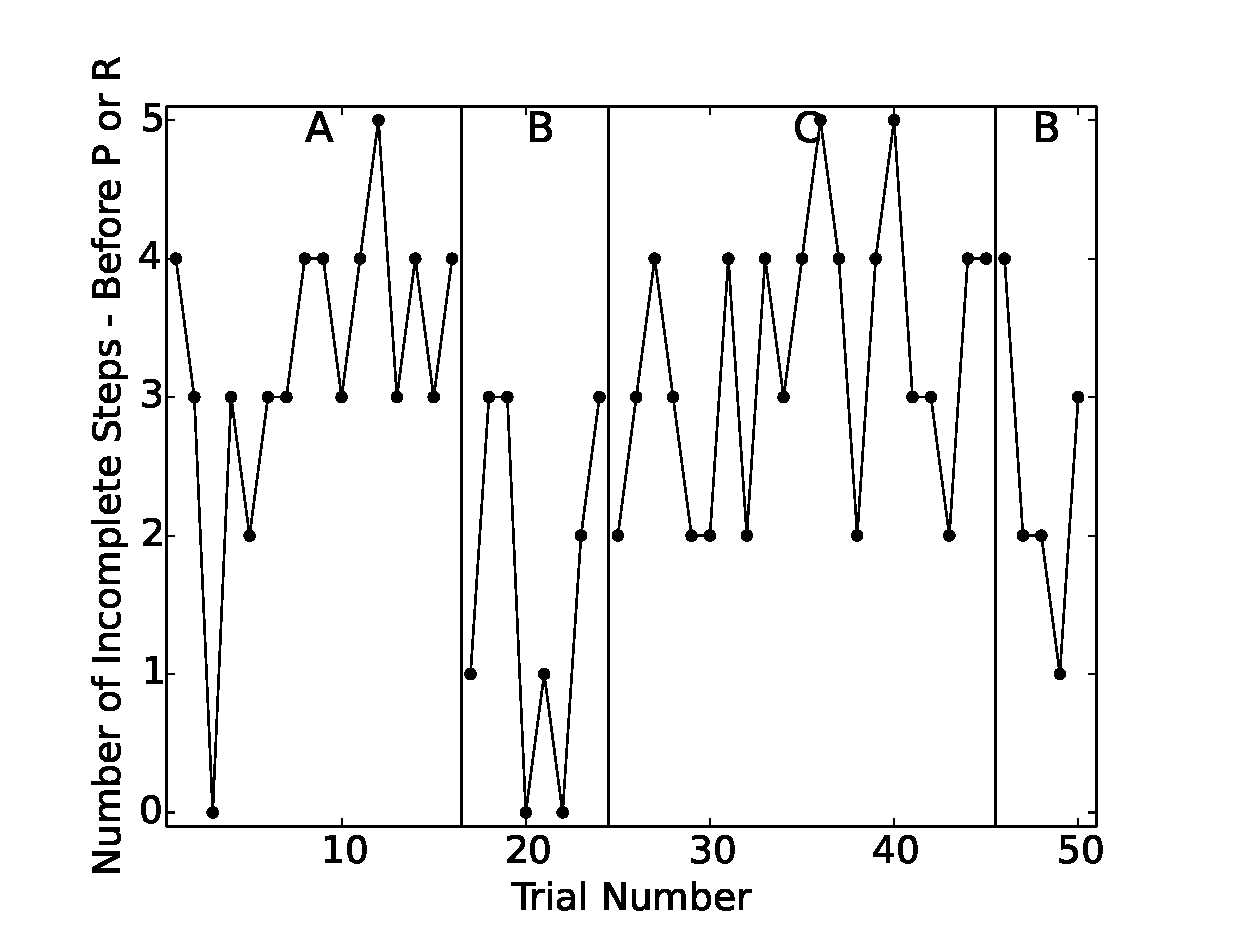
\includegraphics[width=1.1\linewidth]{./img/data_analysis/7NumberofIncompleteSteps-BeforePorR.eps}
		\caption{Total Number of Incomplete Steps - Before Parent or Robot Prompts}
		\label{fig:7TotalNumberofIncompleteSteps-BeforeParentorRobotPrompts}
	\end{subfigure}
	\hfill
	%	~ %add desired spacing between images, e. g. ~, \quad, \qquad, \hfill, or double enter etc.	
	\begin{subfigure}[b]{0.49\textwidth}
		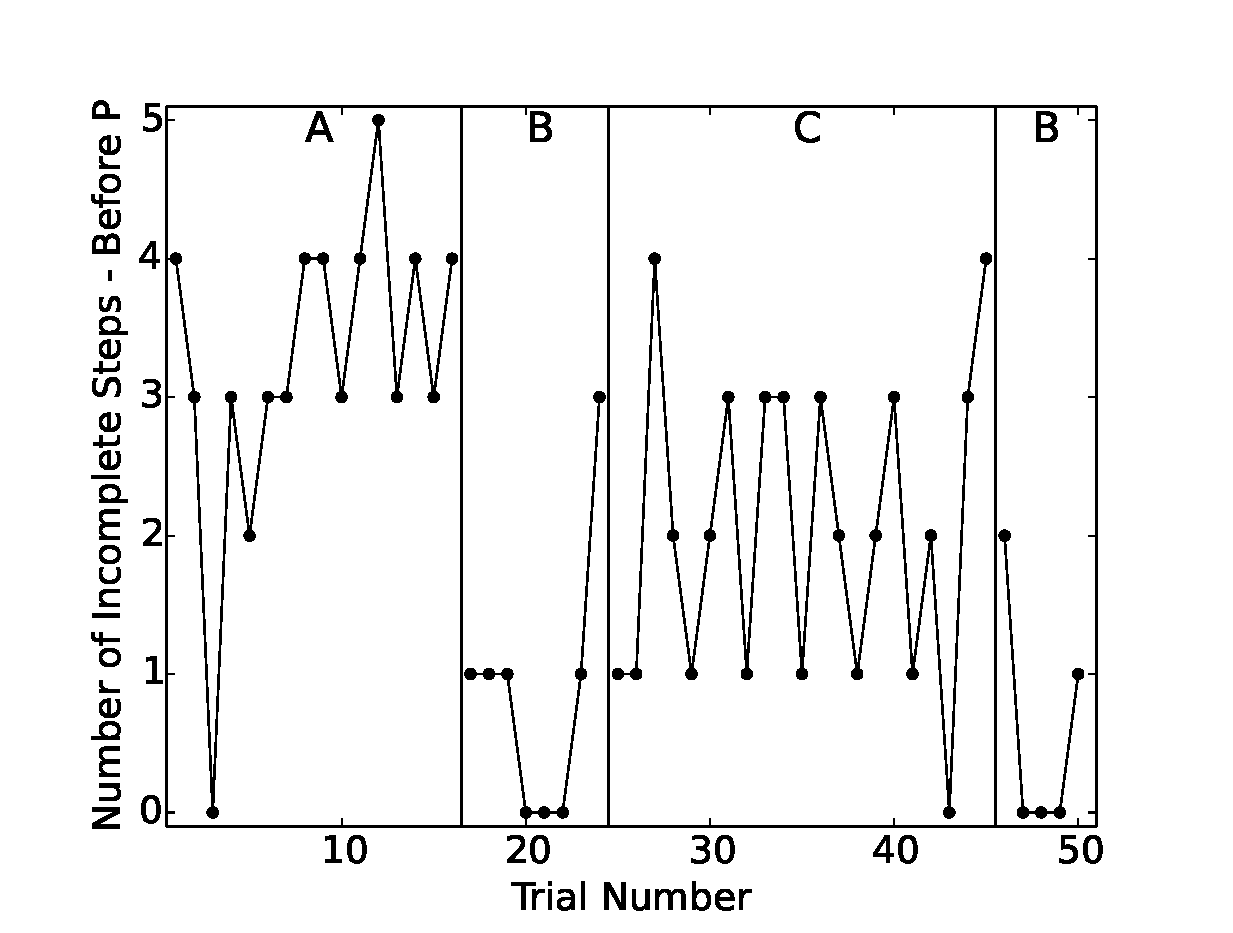
\includegraphics[width=1.1\linewidth]{./img/data_analysis/6NumberofIncompleteSteps-BeforeP.eps}
		\caption{Total Number of Incomplete Steps - Before Parent Prompts}
		\label{fig:6TotalNumberofIncompleteSteps-BeforeParentPrompts}
	\end{subfigure}%
	
	
	\begin{subfigure}[b]{0.49\textwidth}
u		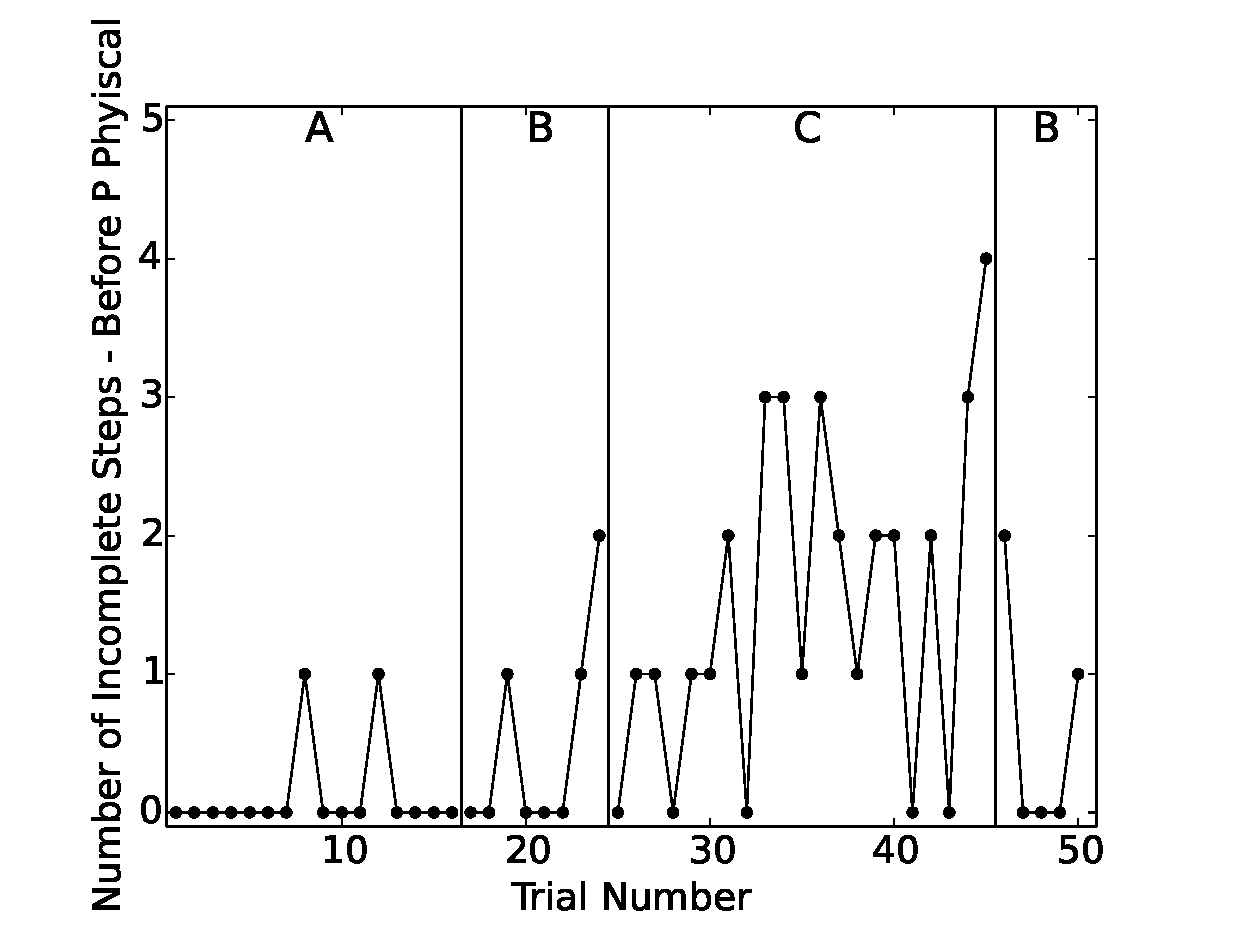
\includegraphics[width=1.1\linewidth]{./img/data_analysis/5NumberofIncompleteSteps-BeforePPhyiscal.eps}
		\caption{Total Number of Incomplete Steps - Before Parent Phyiscal Prompts}
		\label{fig:5TotalNumberofIncompleteSteps-BeforePhyiscalPrompts}
	\end{subfigure}%
	\hfill
	\begin{subfigure}[b]{0.49\textwidth}
		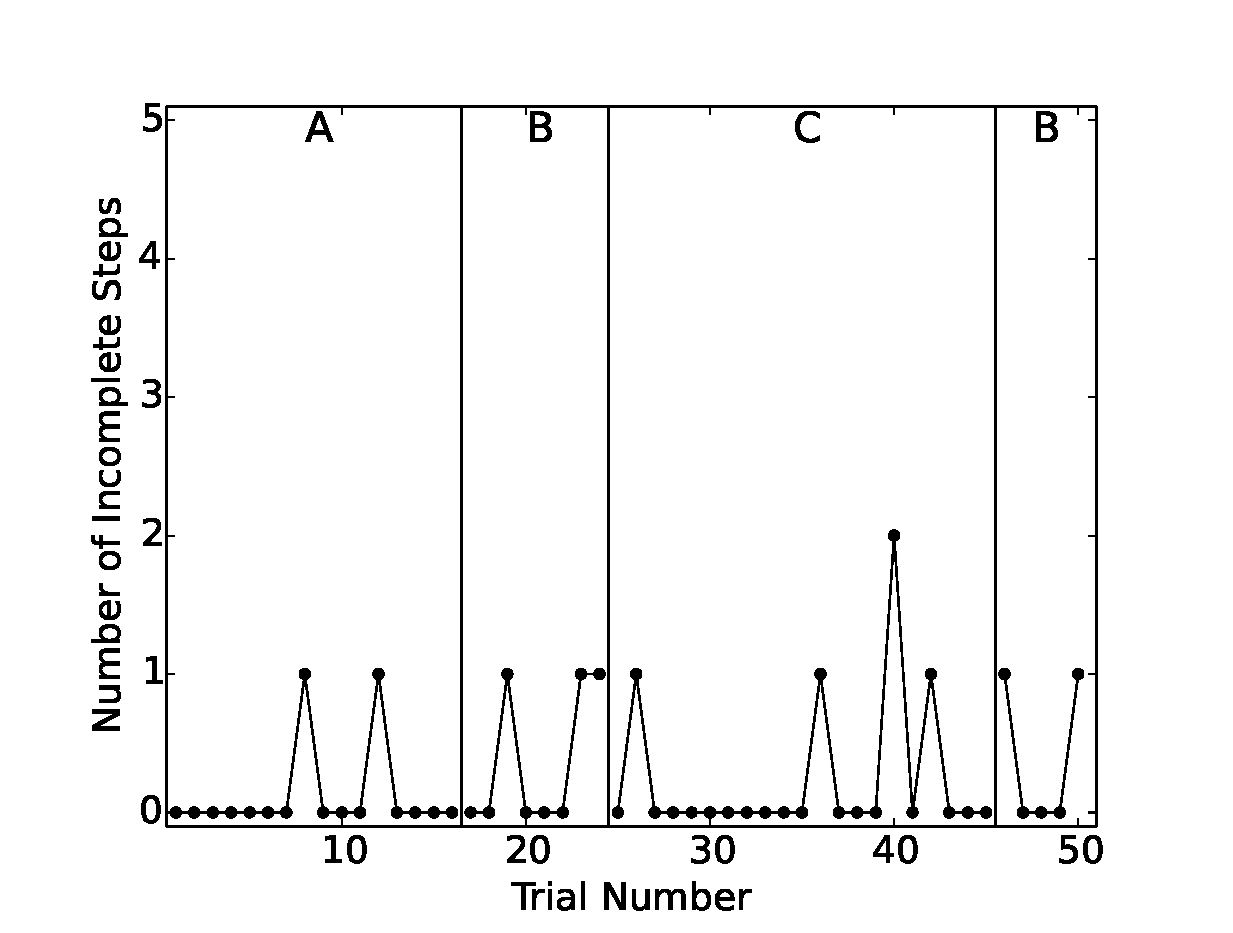
\includegraphics[width=1.1\linewidth]{./img/data_analysis/4NumberofIncompleteSteps.eps}
		\caption{Total Number of Incomplete Steps - Overall}
		\label{fig:4TotalNumberofIncompleteSteps}
	\end{subfigure}%
	\caption{Total Number of Incomplete Steps}
	\label{fig:TotalNumberOfIncompleteSteps}
\end{figure}

\paragraph{Number of Parent Prompts}
The measure ''Total Number of Parent Prompts'' is plotted in Figure \ref{fig:TotalNumberOfParentPrompts}.  Plot \ref{fig:25TotalNumberofParentPrompts} is for the overall count (i.e. counting both physical and non-physical prompts).  It shows that during parent alone phase (A), the measure has an upward trend from 5 moving to 20.  However, in robot alone phase (first Phase B), we have a sudden drop leveling at near zero.  In robot parent phase (C), the measure has a downward trend moving from 15 to 5.  In robot alone repeat phase (second Phase B), we again observe a near zero level.  By comparing the measures across phases, we see that the robot's presence were effective in reducing the number of parent prompts, especially in robot alone and repeat phases.  Plot \ref{fig:26TotalNumberofParentPrompts-Physical} is for the physical prompt count.  This plot shows when the parent resorts to a higher prompt level (i.e. physical prompts such as nudging, guiding, and physically intervene) in order to get the child's compliance.  We see that the level is mainly near zero for all phases except for robot parent phase (C), leveling around 2.5.
\begin{figure}[h]
	\centering
	\begin{subfigure}[b]{0.49\textwidth}
		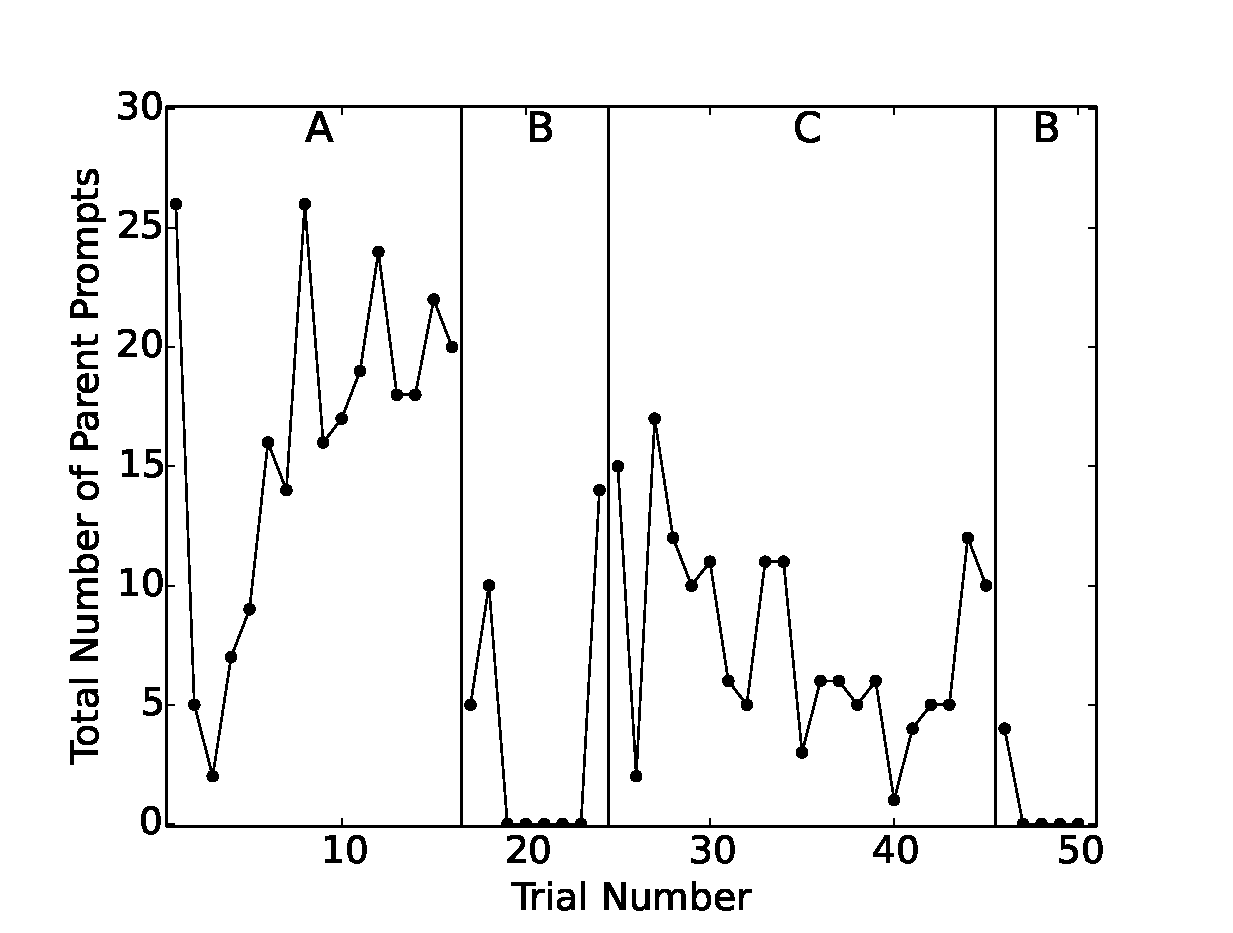
\includegraphics[width=1.1\linewidth]{./img/data_analysis/25TotalNumberofParentPrompts.eps}
		\caption{Total Number of Parent Prompts - Overall}
		\label{fig:25TotalNumberofParentPrompts}
	\end{subfigure}
	\hfill
	\begin{subfigure}[b]{0.49\textwidth}
		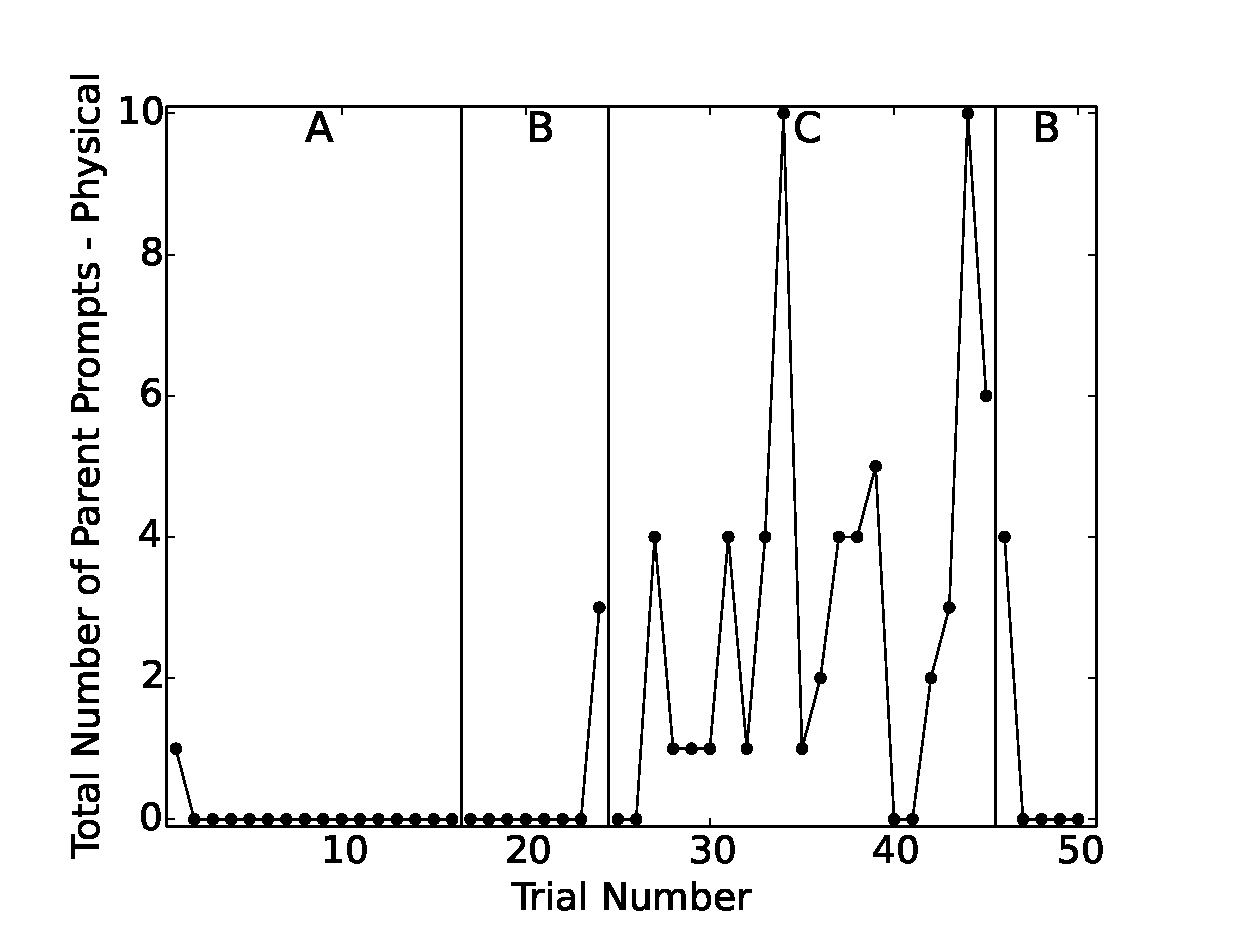
\includegraphics[width=1.1\linewidth]{./img/data_analysis/26TotalNumberofParentPrompts-Physical.eps}
		\caption{Total Number of Parent Prompts - Physical}
		\label{fig:26TotalNumberofParentPrompts-Physical}
	\end{subfigure}%
	\caption{Total Number of Parent Prompts}
	\label{fig:TotalNumberOfParentPrompts}
\end{figure}


\subsubsection{Child's Response to Prompts}
To illustrate the child's different responses to the prompts, we characterized child's responses into three categories: ''compliance'', ''not affected by prompt', and others.

\paragraph{Compliance Rate}
A response is counted towards ''compliance'' if the child executes the correct step in response to the prompt.  If the child was executing the wrong step before prompt, and is converted into doing the correct step due to prompt, we call this hard compliance.  The compliance and hard compliance response rates are shown in Figure \ref{fig:ComplianceRate}.

Plot \ref{fig:102ComplianceRate-Overall} shows the overall compliance rate, with parent alone phase (A) leveling at 80\%, robot alone phase (first Phase B) leveling at 30\%, parent robot phase (C) moving upward from 60\% to 80\%, and robot alone repeat phase (second Phase B) leveling at 80\%.  We see that when the robot was first introduced in robot alone phase (first Phase B), the child did not comply to the prompts.  However, by going through Phase C where the parent prompts for child to follow the robot, the child complies more readily in the robot alone repeat phase, achieving similar level of compliance as the parent alone phase.  We need to note that this plot includes prompts delivered by the robot, by the parent, and by them together.  Even in robot alone and repeat phases, the parent still comes into the washroom and prompts when the child isn't complying to the robot.  To see whether the robot alone can potentially guide the child through the whole hand-washing activity with minimal parent involvement, we plotted the compliance rate counted over only prompts delivered by the robot, shown in Plot \ref{fig:79ComplianceRate-R1Pv0g0}.  This plot confirms the levels observed in the overall plot, validating the improvement of compliance rate seen in R Alone Rep phase.  To investigate to what extent the child is compliant, the overall hard compliance rate is shown in Plot \ref{fig:103HardComplianceRate-Overall}, with parent alone phase (A) split leveling at 100\% and 35\%, robot alone phase (first Phase B) leveling at 25\%.  The robot parent phase (C) averaging around 60\% but the spread increases as trials went on.  Lastly, the robot alone repeat phase (second Phase B) levels at 50\%.  Similar to above, we observe an improvement of hard compliance between robot alone and repeat phases.  Looking at the robot prompts only Plot \ref{fig:92HardComplianceRate-R1Pv0g0}, the robot alone phase (first Phase B) drops to almost 0\%, while robot alone repeat phase (second Phase B) remains at 50\%.
\begin{figure}[h]
	\centering
	\begin{subfigure}[b]{0.49\textwidth}
		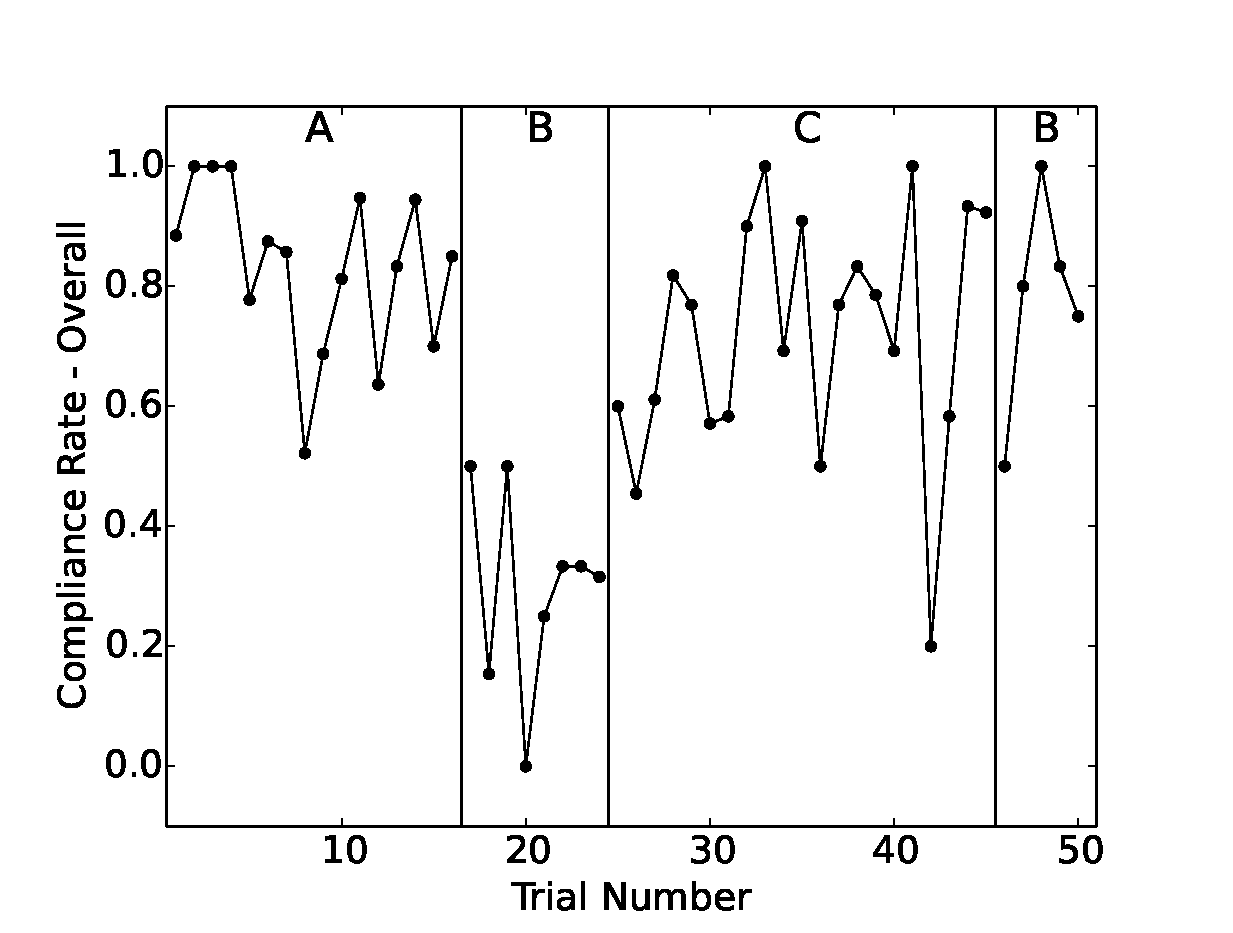
\includegraphics[width=1.1\linewidth]{./img/data_analysis/102ComplianceRate-Overall.eps}
		\caption{Compliance Rate - Overall}
		\label{fig:102ComplianceRate-Overall}
	\end{subfigure}
	\hfill
	\begin{subfigure}[b]{0.49\textwidth}
		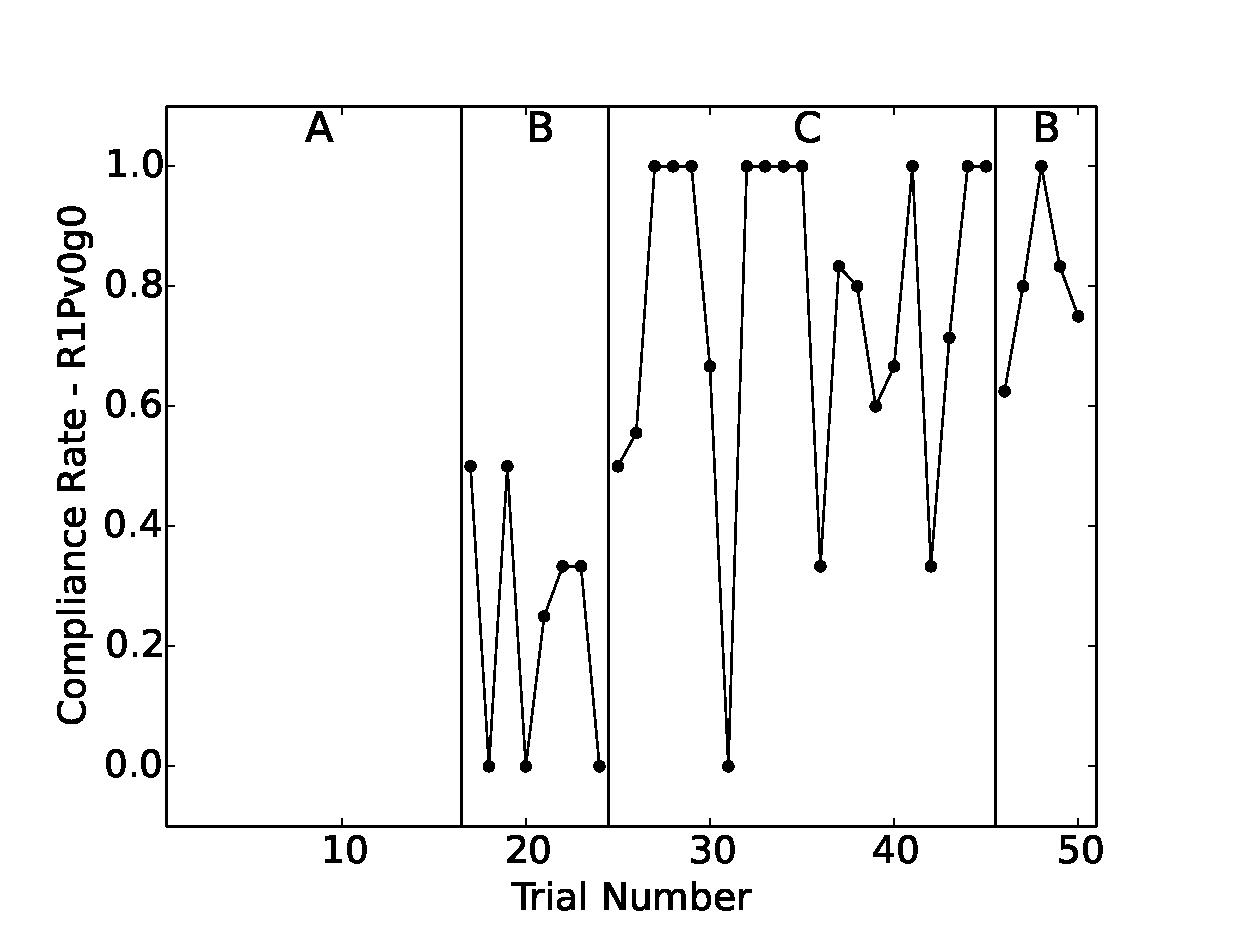
\includegraphics[width=1.1\linewidth]{./img/data_analysis/79ComplianceRate-R1Pv0g0.eps}
		\caption{Compliance Rate - Robot Only Prompts}
		\label{fig:79ComplianceRate-R1Pv0g0}
	\end{subfigure}%
	
	
	\begin{subfigure}[b]{0.49\textwidth}
		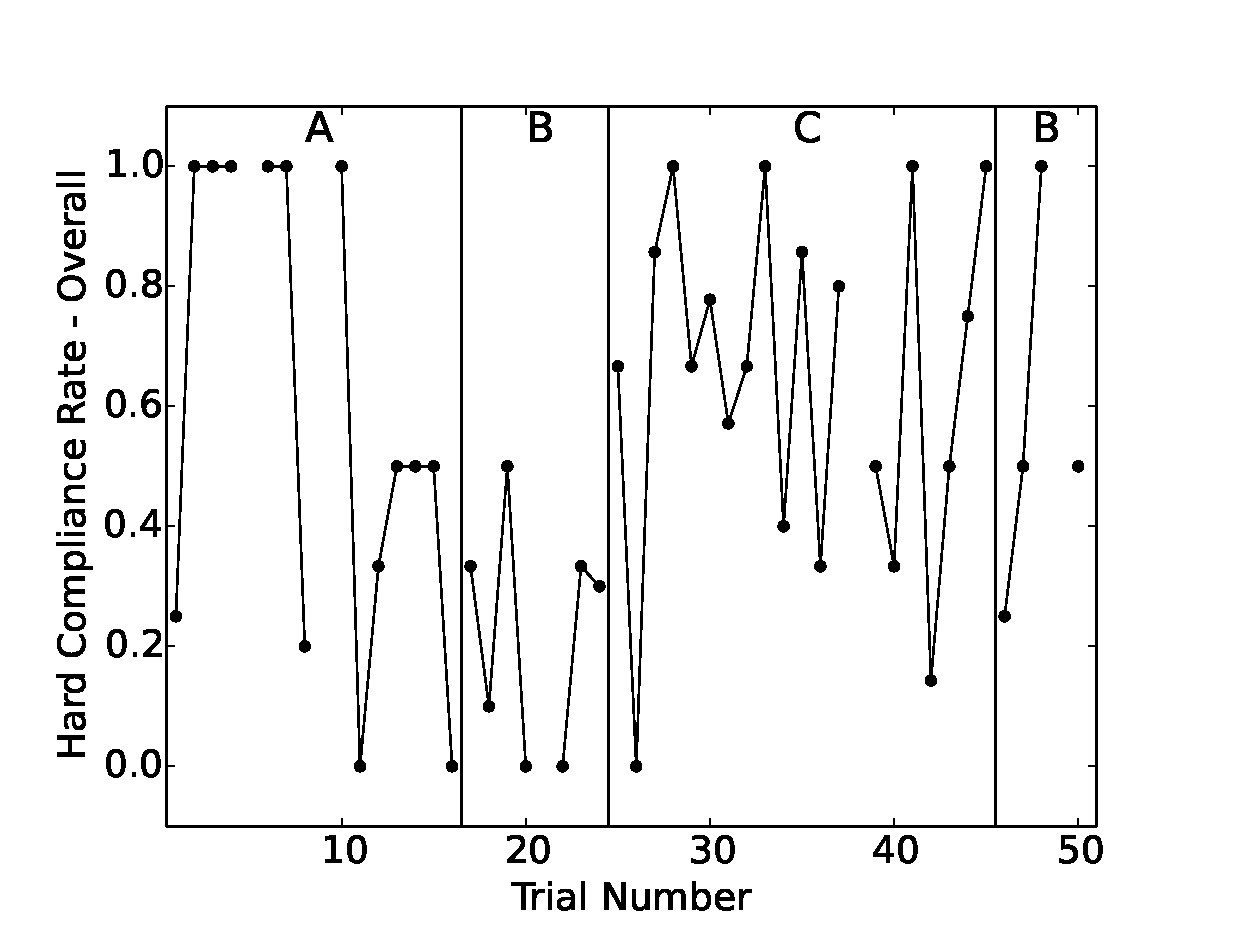
\includegraphics[width=1.1\linewidth]{./img/data_analysis/103HardComplianceRate-Overall.eps}
		\caption{Hard Compliance Rate - Overall}
		\label{fig:103HardComplianceRate-Overall}
	\end{subfigure}
	\hfill
	\begin{subfigure}[b]{0.49\textwidth}
		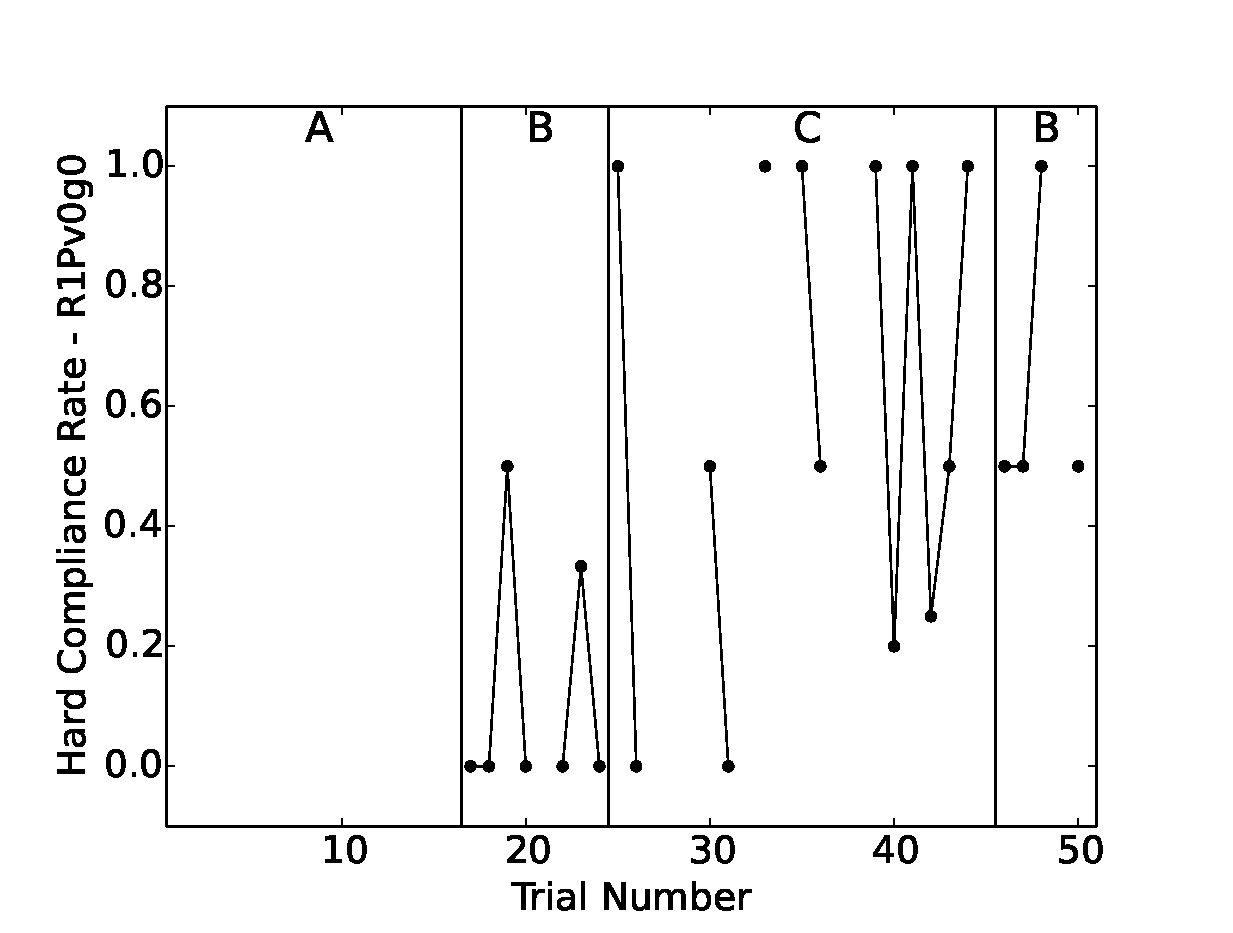
\includegraphics[width=1.1\linewidth]{./img/data_analysis/92HardComplianceRate-R1Pv0g0.eps}
		\caption{Hard Compliance Rate - Robot Only Prompts}
		\label{fig:92HardComplianceRate-R1Pv0g0}
	\end{subfigure}%
	\caption{Compliance Rate}
	\label{fig:ComplianceRate}
\end{figure}

\paragraph{Not Affected By Prompt Rate}
A response is counted towards ''not affected by prompt'' if the child was executing a wrong step and did not change after the prompt or was idling and did not change after the prompt.  The not affected by prompt rate is shown in Plot \ \ref{fig:99NotAffectedByPromptRate-Overall}.  We see that for most phases, it levels at 15\%, but for robot alone repeat phase (second Phase B) it is at 35\%.  This shows the robot prompts were ignored more when the robot was first introduced, but improves to an acceptable level through Phase C.
\begin{figure} [h]
	\centering
	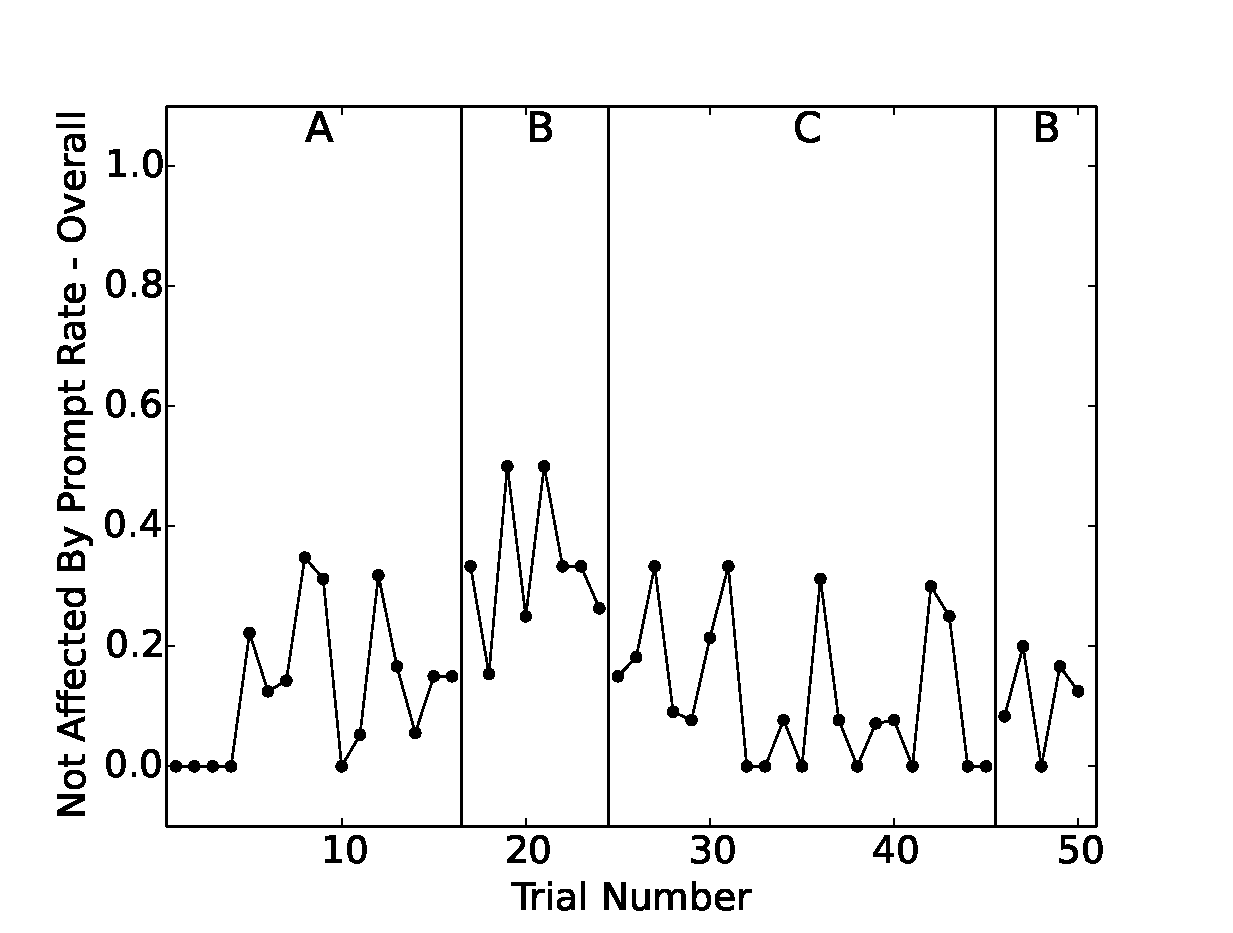
\includegraphics[width=0.6\textwidth]{./img/data_analysis/99NotAffectedByPromptRate-Overall.eps}
	\caption{Not Affected By Prompt Rate}
	\label{fig:99NotAffectedByPromptRate-Overall}
\end{figure}


\subsubsection{Engagement and Visual Attention}
To further characterize child's response to different prompting phases, we investigate how many times the child smiles and murmurs during step execution, and how often the child looks at the prompting agent during prompting and step execution.

\paragraph{Number of Times Child Smiles}
The measure "Total Number of Times Child Smiles" is shown in Plot \ \ref{fig:12TotalNumberofTimesChildSmiles}.  In it, parent alone phase (A) levels at 1.5, robot alone phase (first Phase B) levels at 0.5, robot parent phase (C) has a large spread and averages around 3, and robot alone repeat phase (second Phase B) also has a large spread and averages around 4.  It shows that the child smiles much more in later phases compared to earlier phases, and particularly, smiles in the repeat phase more than in robot alone phase.
\begin{figure} [h]
	\centering
	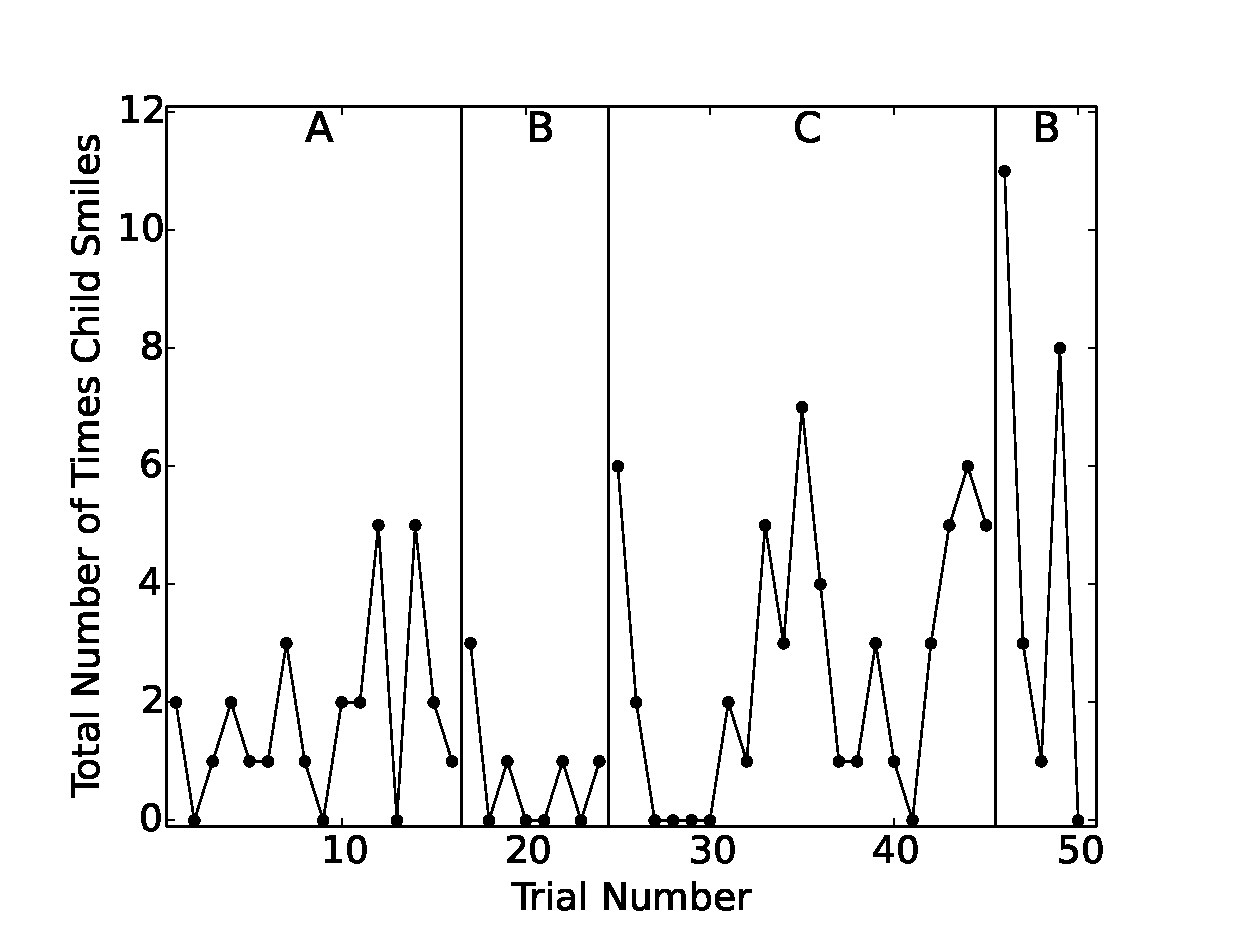
\includegraphics[width=0.6\textwidth]{./img/data_analysis/12TotalNumberofTimesChildSmiles.eps}
	\caption{Total Number of Times Child Smiles}
	\label{fig:12TotalNumberofTimesChildSmiles}
\end{figure}



\paragraph{Number of Times Child Murmurs}
The measure "Total Number of Times Child Murmurs" is shown in Plot \ \ref{fig:13TotalNumberofTimesChildMurmurs}.  In it, parent alone phase (A) has a large spread, averaging around 4.  Robot alone phase (first Phase B) levels at 0.5.  Robot parent phase (C) has a large spread, averaging around 4.  Robot alone repeat phase (second Phase B) levels at 2.  It shows that the child murmurs much more often when the parent is present.  Also, child murmurs in the repeat phase more than the robot alone phase.
\begin{figure} [h]
	\centering
	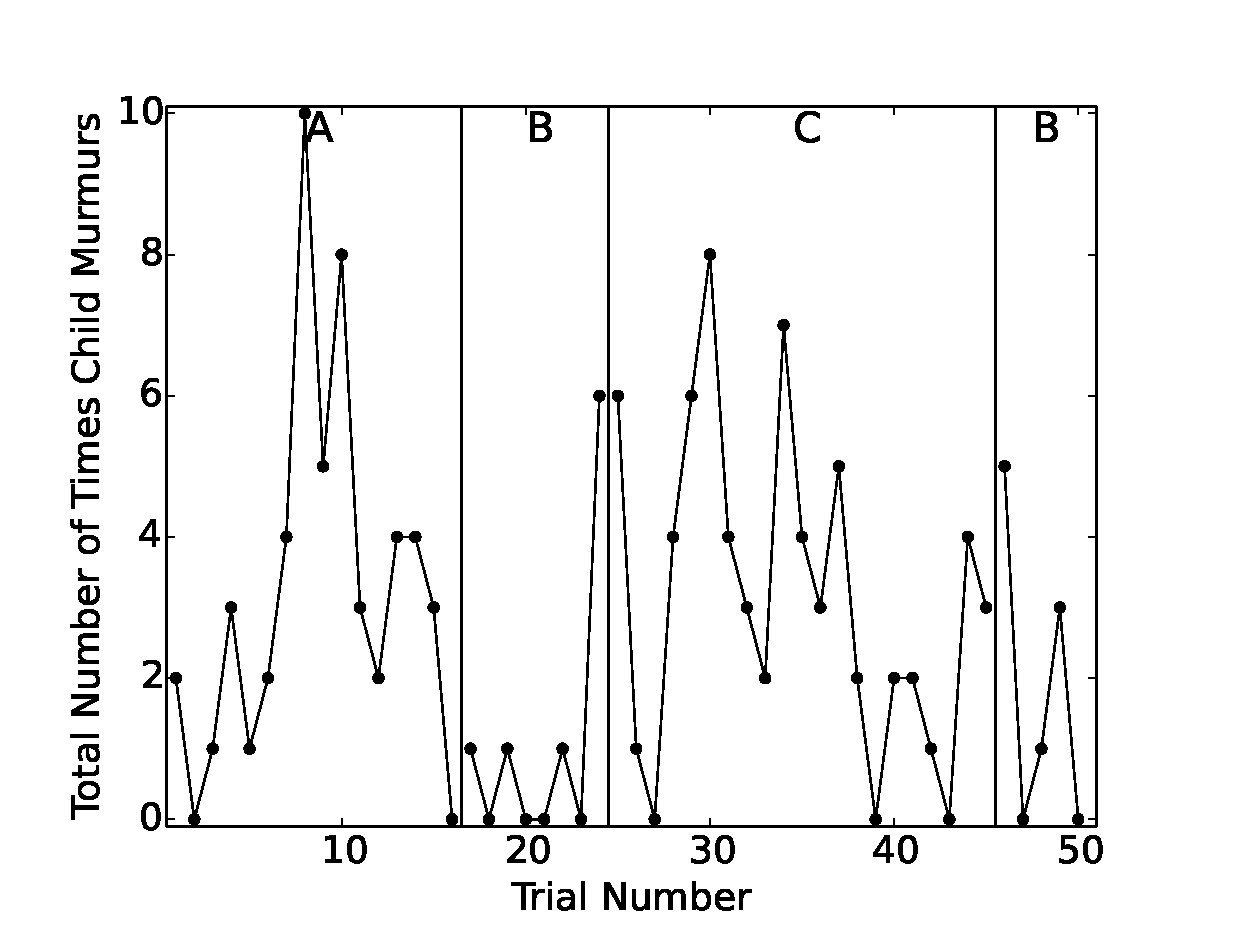
\includegraphics[width=0.6\textwidth]{./img/data_analysis/13TotalNumberofTimesChildMurmurs.eps}
	\caption{Total Number of Times Child Murmurs}
	\label{fig:13TotalNumberofTimesChildMurmurs}
\end{figure}

\paragraph{Looking at Prompting Agent Rate}
A prompt can be given by the parent, by the robot, or by them together.  During prompting and during step execution, the child may turn and look at the parent and/or the robot.  The gaze behavior of the child is shown in Figure \ref{fig:LookingAtPromptingAgentDuringPrompts} for all the cases above.  Because not all cases have the same amount of data in all phases, we will only mention here the phases that have enough evidence.  In Plot \ref{fig:8LookingatParentRateGivenParentPrompted}, ''Looking at Parent Rate - Given Parent Prompted'' levels at 40\% in parent alone phase (A).  In Plot \ref{fig:92HardComplianceRate-R1Pv0g0}, ''Looking at Robot Rate - Given Robot Prompted'' trends downward from 50\% to 30\% for robot alone phase (first Phase B), levels at 30\% with high spread for robot parent phase (C), and levels at 20\% for robot alone repeat phase (second Phase B).  We see that when the parent and the robot prompt individually, the parent has a higher chance of getting the child's visual attention.  Although the robot had similar levels of attention when was first introduced, it dropped as the study went on.  In Plot \ref{fig:10LookingatParentRateGivenBothPrompted}, ''Looking at Parent Rate - Given Both Prompted'' averages around 50\% with high spread in robot parent phase (C).  In Plot \ref{fig:11LookingatRobotRateGivenBothPrompted}, ''Looking at Robot Rate - Given Both Prompted' levels at 15\% for robot parent phase (C).  We see that when the parent and the robot prompt at the same time, the parent had a greater amount of visual attention.  It is interesting to note that the parent had similar levels of visual attention when prompting alone and when prompting with the robot.  The robot, however, experienced a decrease in visual attention level when the parent prompts with it.
\begin{figure}[h]
	\centering
	\begin{subfigure}[b]{0.49\textwidth}
		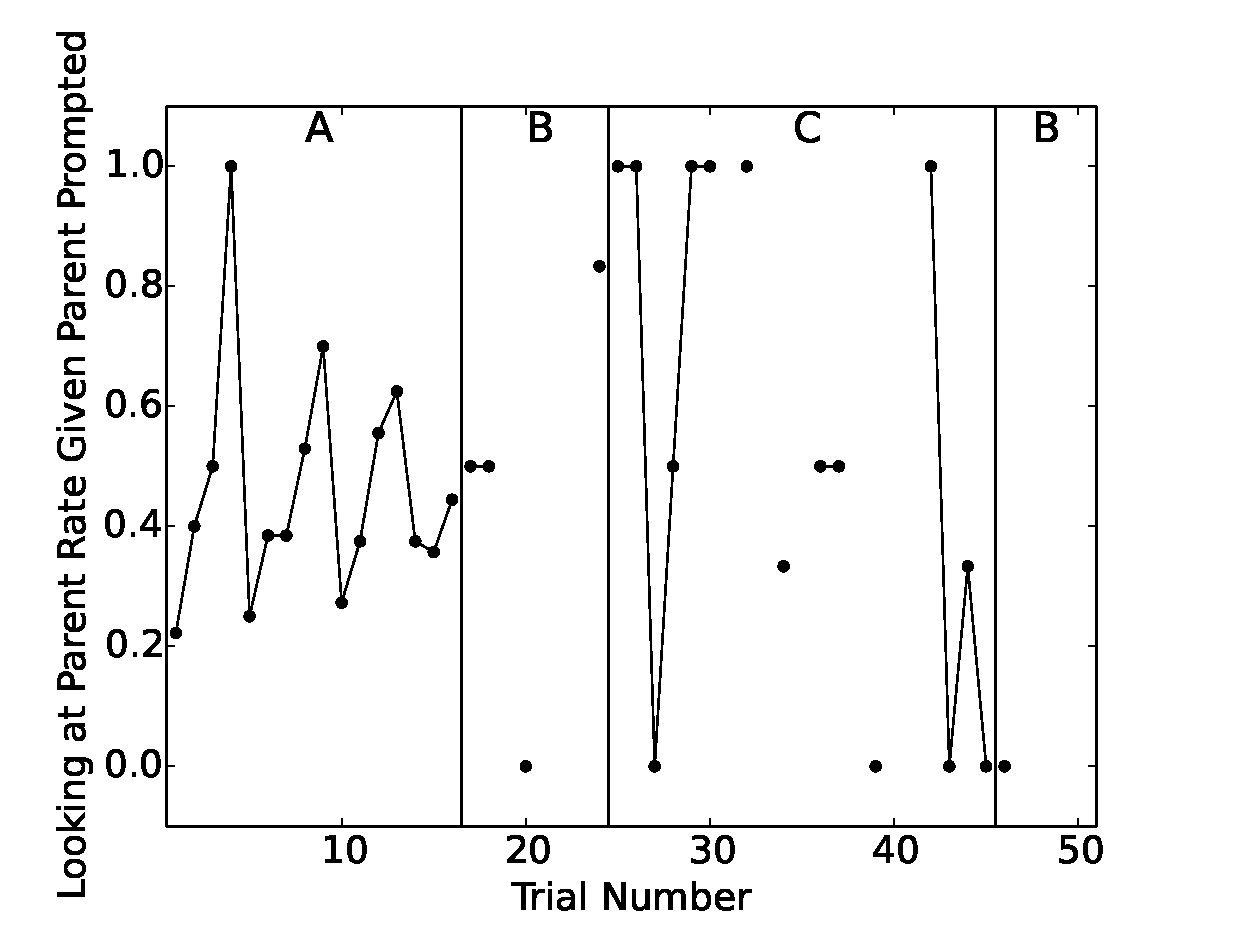
\includegraphics[width=1.1\linewidth]{./img/data_analysis/8LookingatParentRateGivenParentPrompted.eps}
		\caption{Looking at Parent Rate - Given Parent Prompted}
		\label{fig:8LookingatParentRateGivenParentPrompted}
	\end{subfigure}
	\hfill
	\begin{subfigure}[b]{0.49\textwidth}
		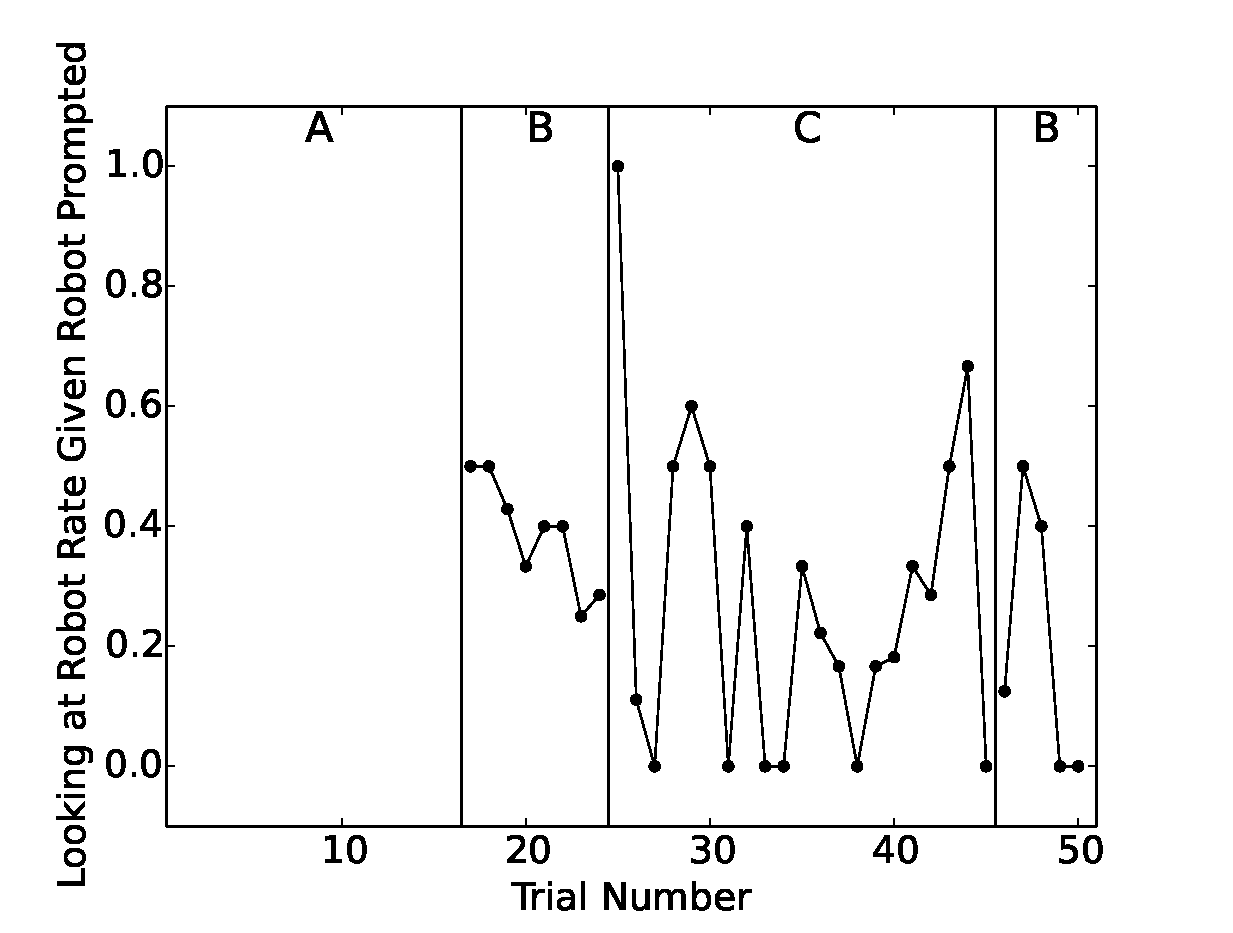
\includegraphics[width=1.1\linewidth]{./img/data_analysis/9LookingatRobotRateGivenRobotPrompted.eps}
		\caption{Looking at Robot Rate - Given Robot Prompted}
		\label{fig:9LookingatRobotRateGivenRobotPrompted}
	\end{subfigure}%
	
	
	\begin{subfigure}[b]{0.49\textwidth}
		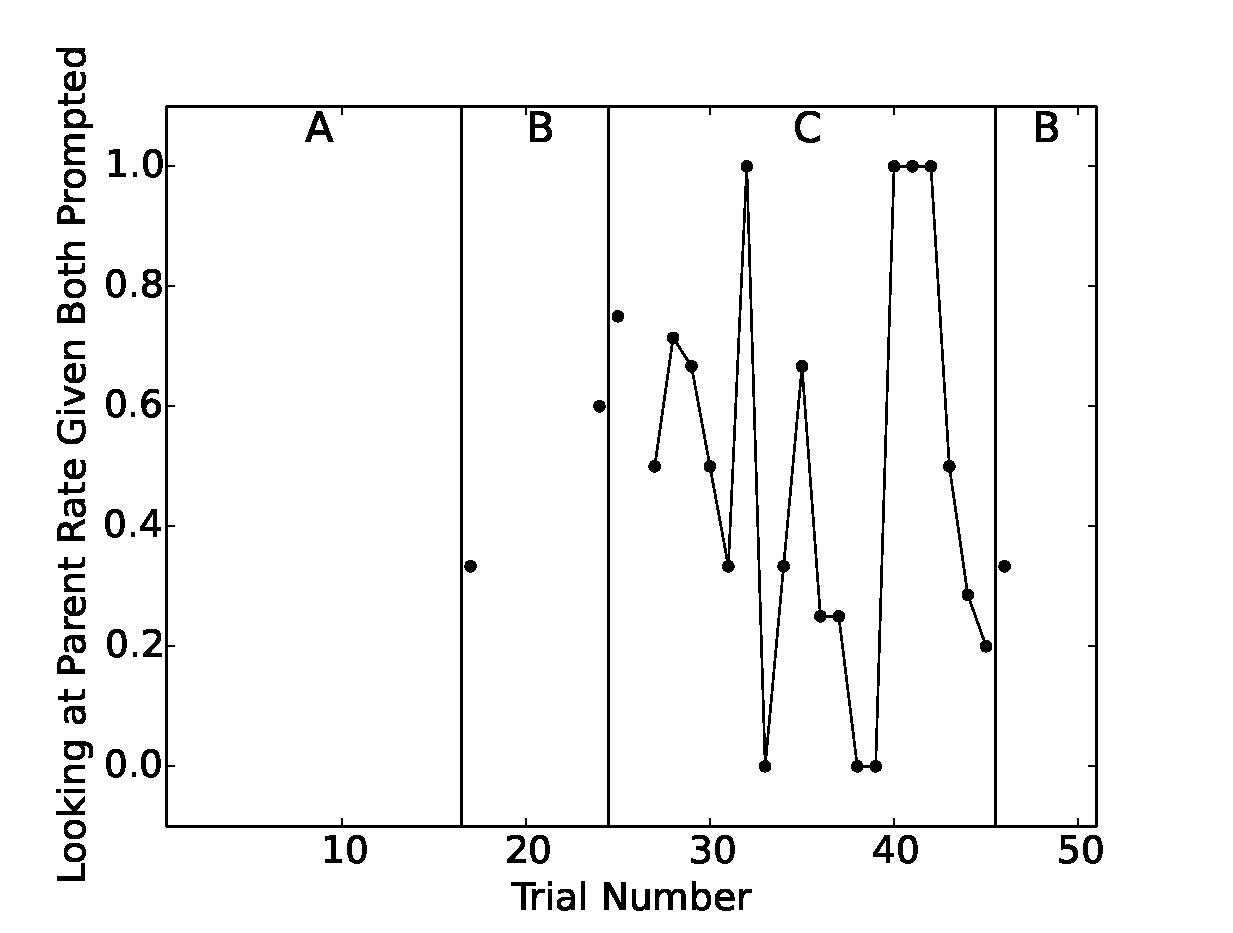
\includegraphics[width=1.1\linewidth]{./img/data_analysis/10LookingatParentRateGivenBothPrompted.eps}
		\caption{Looking at Parent Rate - Given Both Prompted}
		\label{fig:10LookingatParentRateGivenBothPrompted}
	\end{subfigure}
	\hfill
	\begin{subfigure}[b]{0.49\textwidth}
		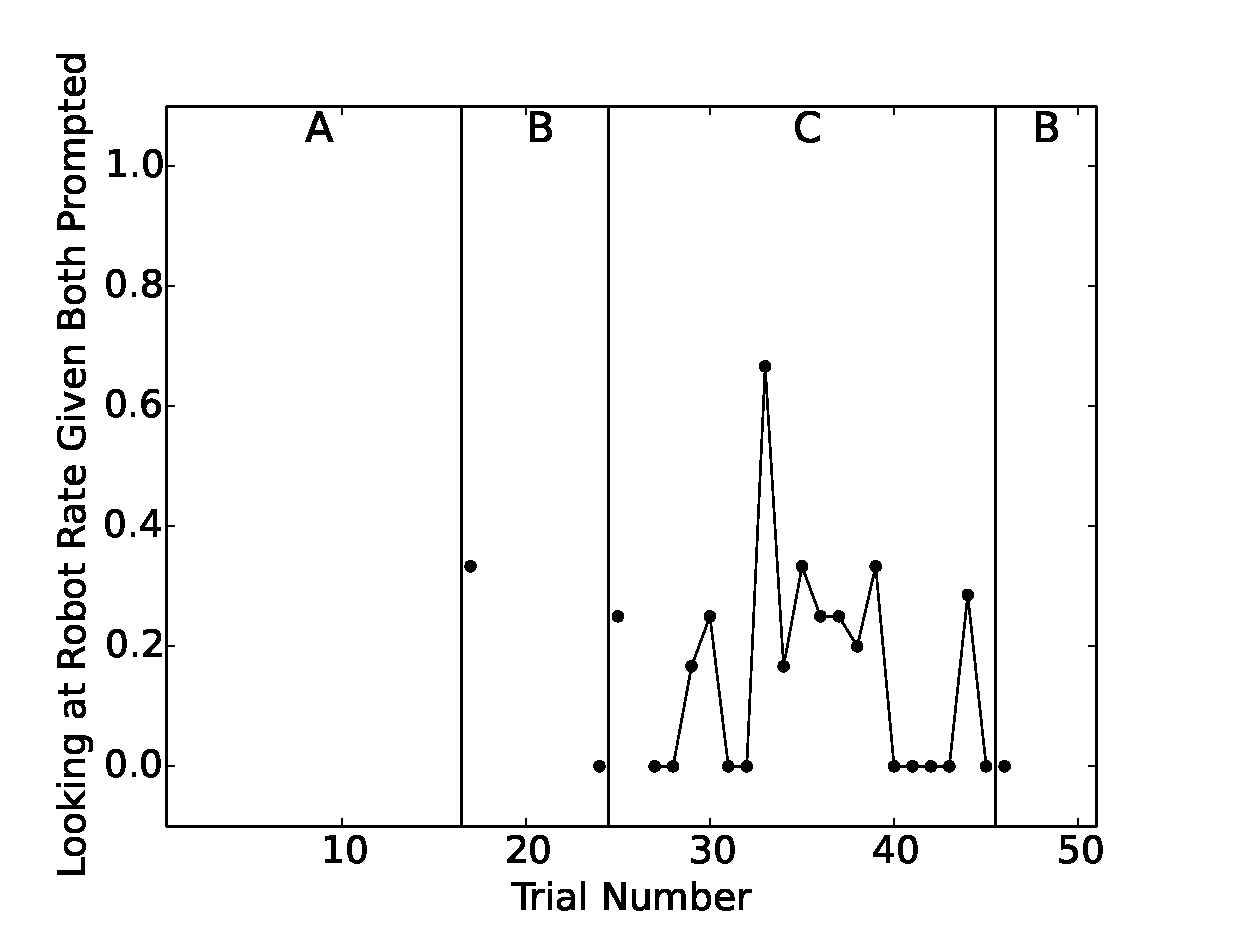
\includegraphics[width=1.1\linewidth]{./img/data_analysis/11LookingatRobotRateGivenBothPrompted.eps}
		\caption{Looking at Robot Rate - Given Both Prompted}
		\label{fig:11LookingatRobotRateGivenBothPrompted}
	\end{subfigure}%
	\caption{Looking at Prompting Agent Rate}
	\label{fig:LookingAtPromptingAgentDuringPrompts}
\end{figure}

\subsection{Survey Data Results}

\subsubsection{Entrance Survey}
The entrance survey results are reported as follows:

\paragraph{Child's Experience with Technologies}
The child is more of a visual learner.  He uses a computer at home, and likes to use it very much.  He also likes to use other technologies (e.g. iPhone, iPad), and likes to watch movies and TV.  He doesn't have a robot toy to play with at home or at school, so the parent doesn't know how much he likes to play with robot toys.  The parent never used technologies to help the child with self-care activities except using pictures to teach step by step hand-washing.

\paragraph{Child's Personal Preferences}
The child is sensitive to sound.  He likes Disney cartoon musics, and likes to watch his favorite cartoon scenes repeatedly on the iPad.  To reward the child after a good behavior, the parent suggested the following rewards: give extra time to play on iPad, give him praises (e.g. good job), give children books to read and animal dinosaurs to play with, give the parent's iPhone since his favorite musics are on there.

\paragraph{Child's Abilities on Hand-washing and on Other ADLs}
The parent agrees that the child usually gets distracted when performing hand-washing.  To assist him, the parent mainly reminds him to put soap, rinse properly, and dry properly with towel.  He needs more prompting in these areas since he always washes in a hurry.

Other activities the child needs help with include:  tooth brushing -- 2 hours/week; bathing -- 4.5 hours/week; dressing -- usually just hand the clothes to him, he knows how to put them on, but needs reminders of the order of the clothing, 7 hours/week.

\paragraph{Parent's Expectation and Concerns}
The parent expected the robot to be helpful in reminding the child to put soap, rinse and dry more, similar to the role of the parent.  Some concerns the parent has include: the child may be wondering why does he need to wash hands so many times repeatedly; the child performs well in his comfort zone with the same environment, so it takes a while for the child to get used to the lab environment.


\subsubsection{Post-Intervention Survey for Parent}
The post-intervention survey results are presented in Table \ref{tab:PostInterventionSurveyData}.  We see that the parent was happy with all aspects of the robot as a prompting agent, but did not see it to be as good as herself yet.  The suggestions the parent made regarding the robot and the experiment are reported in the discussion section.

\begin{table}[h]
	\centering
	\begin{tabular}{ | p{12cm} | l | }
		\hline
		\textbf{Survey Question}	&	\textbf{Parent's Answer}	\\	\hline	\hline		
		Hand-washing steps break down was appropriate	&	Strongly Agree	\\	\hline
		My child understood the verbal prompts	&	Agree	\\	\hline
		Robot's verbal prompts were appropriate	&	Strongly Agree	\\	\hline
		The prompt wordings were similar to mine	&	Strongly Agree	\\	\hline
		The prompt voice and tone were appropriate	&	Strongly Agree	\\	\hline
		The prompt wordings were easy to understand	&	Strongly Agree \\	\hline
		My child understood the gesture prompts	&	Strongly Agree	\\	\hline
		The gesture prompts were appropriate	&	Strongly Agree	\\	\hline
		The gesture prompts were easy to understand	&	Agree	\\	\hline
		The physical appearance of robot is aesthetically pleasing	&	Agree	\\	\hline
		The attention grabber gestures were appropriate	&	Strongly Agree	\\	\hline
		The verbal rewards were appropriate	&	Strongly Agree	\\	\hline
		The reward gestures were appropriate	&	Strongly Agree	\\	\hline
		The robot was effective in assisting my child through hand-washing	&	Strongly Agree	\\	\hline
		The robot motivated my child to wash hands	&	Strongly Agree	\\	\hline
		The robot was fun for my child to use	&	Strongly Agree	\\	\hline
		My child was confused by the robot	&	Disagree	\\	\hline
		I like the idea of a robot prompting my child	&	Strongly Agree	\\	\hline
		The robot is able to provide guidance as well as I can or better	&	Neither Agree or Disagree	\\	\hline
		I would want to own a robot like this one	&	Strongly Agree	\\	\hline
	\end{tabular}
	\caption{The Post-Intervention Survey Data}
	\label{tab:PostInterventionSurveyData}
\end{table}
\section{Discussion}
A Wizard of Oz study has been conducted following the A-B-C-B case study design on a single participant.  In Phase A, the parent alone prompted the child through hand-washing steps.  In first Phase B, the robot alone prompted the child.  In Phase C, the parent and the robot jointly prompted.  In second Phase B, the robot alone prompted the child again.  Parent researcher interview was conducted during breaks between trials.  Both qualitative and quantitative analyses were conducted on the study data, and we observed promising results.


\subsection{Summary of Results}
We saw that, although the child did not listen to the robot as much as it did to the parent when the robot was first introduced, through a parent robot joint training phase, the child showed drastic improvement in robot prompt compliance, approaching the compliance level achieved by the parent prompts.  Although our participant did not appear to need help in how to execute each hand-washing steps, he did need prompting to get the hand-washing started and stay on task, and supervision on scrubbing, rinsing and drying longer and not getting too much soap.  Our analyses showed that through training, the robot was able to achieve getting the child to meet most of these goals.  Specifically, the child waited for the robot to prompt first before starting the hand-washing activity.  Also, the child followed the robot's rinse prompts and rinsed longer as a result.  However, the robot was only somewhat successful in getting the child to move on from the soap step, and was unsuccessful in getting the child to scrub hands or to dry hands longer.  The parent, on the other hand, had no problems in getting the child to scrub hands, but she did have some difficulties in getting the child to dry longer and had definite difficulties in getting the child to move on from the soap step.  

The parent was not instructed in the specifics of how to prompt -- she prompted in the most natural way she and the child were used to, and yet there were a lot of similarities between the parent and the robot's prompting patterns.  First, they shared similar breakdown of the hand-washing steps, although the parent referred to the scrub step as lather.  In addition, the both the parent and the robot prompted by giving verbal instructions along with some form of gesture prompts.  The differences were that the parent used more pointing and less motion demonstration, and that the motion demonstrations from the parent were much faster moving than the robot's (especially for the scrub step).  The child paid much more attention to the parent's faster moving motion demonstrations than the robot's, and is one area of future improvements.  Other design recommendations for the robot included faster response times to child's behaviors, issuing a fast attention grabber accompanied with increased severity in tone of voice when the child is non-compliant, and rewarding the child for major steps only (e.g. the end of rinsing and drying steps).  Other design recommendations raised by the parent and the researcher mainly involved engaging the child better, including more dynamic motions for gestures, playing cartoon noises for rewards or attention grabbers, having a bigger robot so it is more visually engaging, etc.

In terms of modes of interactions needed between the child and the robot for successfully helping the child to wash hands, the delivering of verbal and gestural prompts with at least two levels of severity (more severe sounding and looking prompts delivered when the child is non-compliant) were definitely needed.  However, the detection of the visual focus of attention of the child showed little value.  The child's visual attention was hardly an indicator of engagement at all.  On the other hand, we found that understanding verbal feedbacks from the child may be useful as the child verbally repeated instructions when he was processing them, and murmured back in protest when he did not wish to follow certain prompts.  Utilizing these speeches as indication of the child's engagement may be useful in adjusting robot prompts to better suit the child's needs.  Also, we observed that the child did not like prolonged rinsing, and what the parent did was to stop prompting the rinse step and to move on to the next step when the child showed non-compliant behavior through rinsing for only a second and quickly removing his hands from the water.  The robot did not move on and repeated the rinse prompts in hope the child would follow, and as a result, the child often moved on by himself without waiting for the robot.  In future studies, the robot should also implement a way to work with the child to rinse as much as possible but learn to move on when the child shows signs of non-compliance.


\subsection{Internal and External Validity}
In this section, our results are critically reviewed based on data collection, analysis methods, and result interpretations.  Possible sources of errors, competing interpretations, limitations of results, and their generalizability are discussed.

\subsubsection{Quantitative Analysis Method}
The choice of measures used in the quantitative analyses were based on our study objectives and chosen in light of the qualitative analysis results, in an attempt to answer the question ``Is the robot NAO able to guide our participant, a child with ASD, through hand-washing?".  ``Number of Steps Completed'' only reflected the variety of steps completed, but did not measure the quality of the completed steps.  Thus it could only partially confirm how well the robot guided the child.  ``Longest Duration of Rinse Step'' was our attempt to measure the quality of the rinse step completed.  The rinse step was chosen due to the drastic improvement the child exhibited on this particular step, and the duration of the longest rinse was the most obvious way to measure the quality of the rinse step completion.  One thing to note is, the parent, during the training phase, focused most of her prompts on getting the child to follow the rinse prompts from the robot, but very little prompts were focused on the dry hands prompts.  Consequently, we did not experience as much improvement on the duration of dry hands step.  To link the child's success in completing all steps and with good quality to the prompting agents, the ``Compliance Rate'' and the ``Not Affected By Prompt Rate'' were measured, for all steps (and Compliance Rate for the rinse step particularly as well).  We see that the robot had much more influence on the child in second Phase B, but not in first Phase B, and this resulted in an increased duration of rinse in second Phase B.  Thus, we concluded that the robot was successful in improving the quality of hand-washing of our child with ASD.  But since the child already knew all the steps and was able to complete all steps in first Phase B with minimal influence from the robot, no conclusions can be made regarding whether the robot could successfully teach our child with ASD a new hand-washing step.

Medians were used as a fair and reliable way of comparing the measures across phases.  The choice of median, as opposed to mean, was out of the consideration for robustness against outliers.  This may be a good choice if the data had relatively low variance and few outliers.  However, our data contained high variance, and the definition of outliers became blurred.  Take ``Rinse Step Compliance Rate'' (seen in Figure \ref{fig:5ComplianceRate-RinseStep}) for example.  The rate in Phase C has a median of 100\%, but there are a third of data points in this phase falling below 80\%.  Thus, one obvious question is, why have we not used some form of description of variance alongside our description of data centers (i.e. median) in our across phase comparisons?  The reasoning was that the low sample size for some phases (e.g. second Phase B only has 5 data points) made any analysis based on variance not statistical significant.  This is a limitation of our study results, but given the pilot nature of our study, it is acceptable since it yielded promising results confirming the direction of future studies.

Another limitation exists in our lack of control on video data annotation errors.  For a more rigorous future study, more than one person should carry out the data annotations, and the degree of annotator subjectiveness can then be characterized by an inter-rater agreement measure such as the Cohen's Kappa \cite{volkmar2005handbook}.

\subsubsection{Qualitative Analysis Method}
The qualitative analyses of our study employed several strategies to ensure internal validity.  These strategies being reviewed include triangulation, member checks, adequate engagement in data collection, reseracher's position or reflexivity, peer review / examination, audit trial, rich thick description, an maximum variation \cite{merriam2014qualitative}.  Firstly, we employed triangulation by using multiple investigators and sources of data to confirm findings.  The observations of the child's behaviors and possible robot design recommendations were made by the researcher through making field notes of the trials video data, by the parents through the parent researcher interview discussions and the post intervention survey.  Secondly, during the parent researcher interviews, due to the interactive nature of the interview format, the member check technique was inherent.  The researcher was able to check his understanding of the emerging findings with the parent to ensure minimal misinterpretation was made.  Thirdly, we did not employ the adequate engagement in data collection technique satisfactorily.  Phase A and first Phase B were carried out long enough to see saturation of findings, but due to limitation of time, training Phase C and second Phase B were not carried long enough to such saturation.  Especially, the training Phase C could have been longer to see possibly even further improvement of the child, and the second phase C could have been longer (at least to match the length of the first Phase B) to eliminate any doubts that the improvements observed in training phase were successfully retained.  In regards to researcher's position or reflexivity, the researcher must confess that he has little training in research with children with ASD or in any general human behaviors research.  Such lack of experience may prove invalid any opinion the researcher had on the child's behaviors and on the reasons behind them.  However, the researcher relied heavily on the parents' interpretation of the child's behaviors, preferences, and possible reasons behind his behaviors instead.  And the parents, being both experienced with the child's needs in particular and trained with knowledges of children with ASD in general, were very adequate observers used by our study.  In addition, audit trail and rich, thick descriptions were used to compensate the researcher's interpretation errors.  By providing a detailed account of the backgrounds, methods, procedures, and decisions made when conducting the study, the value of the study results can be critically assessed based on contexts by other researchers themselves when reading this thesis.  Lastly, during the training phase, the parent involvements were purposefully varied through the phase.  This maximum variation technique allowed greater diversity in sample selection, enabling a greater range of findings and possible applications of the findings.

\subsubsection{Confounding Variables}
Due to the study protocol and the research design, there were several uncontrolled variables that may have confounded our results, threatening the internal validity of our results.

One confounding variable was the change of robot control scheme in the middle of the first Phase B.  The reason for change was because our participant required a much more reactive robot who can switch the current step being prompted on the fly.  As stated in the study protocol, if any essential improvements of the robot (or the study procedures) were made apparent through the ongoing analysis, we would implement the change.  After the control scheme switch, both the parent and the robot operator (the researcher) felt the robot was more responsive to the child.  However, the parent did report that the robot was still too slow for the child, and sometimes the pause between robot actions were still too long.  This confounding variable had a sudden change, and we expected to also see sudden changes in our dependent measures shortly following the effect.  However, this was not observed, and may be due to the effect size of this confounding variable was too low compared to the level of noises in our measures.  Another possibility is that some inherent nature of the child made him remaining to behave a certain way despite changes in stimulus.  Either way, this confounding variable does not threaten our results that the robot was eventually able to help the child through hand-washings.  However, it may threaten the hypothesis that it was the training phase instead of the robot control scheme change that caused the improvements in the child's behaviors towards the robot.

Another confounding variable was the fact that the current study (Wizard of Oz) involved a human operator (the researcher) remotely controlling the robot.  The researcher had no experience guiding the participant through hand-washing prior to the study, and thus it was a learning process for the researcher through out the study as well.  This meant that the researcher changed the order of steps the robot prompts were delivered to best fit the child's preference (e.g. the child preferred to put on soap before turning on water).  Also, the researcher chose prompts that were more effective (e.g. the attention grabber was not effective and so was not used in the end, and the child did not distinguish between scrub hands and rinse hands, so scrub hand prompts were not used in the end).  These changes were gradual, but may play a confounding effect on our measures, threatening the hypothesis that the training phase was the sole cause of the child's improvements.  In addition, in the future when we will be automating the robot behaviors, tuning the robot prompts and order of steps to each child's preference will be an inevitable part of the automation process.

The researcher was not the only one learning, the child in fact was learning and familiarizing with the robot prompts, the experiment environment, and the hand-washing activity in this environment.  Children with ASD are very peculiar about keeping routines in a familiar environment.  Thus, introducing the robot, which the child did not have any prior experience to playing with or following orders from, in a foreign washroom with unfamiliar washroom setups, created a barrier for the child to put on his best responses to the robot prompts.  Since the parent alone prompting phase (Phase A) also had the unfamiliarity of environment confounding effect, this confounding variable does not threaten the conclusion that the robot did not perform as well as the parent as a prompting agent.  But the reason for this inequality in performance can be explained by the robot being inferior to the parent as a prompting agent by nature, or can be explained by the fact that the child was much used to following orders from the parent than the robot.  In addition, the child's unfamiliarity and learning to get used to being prompted by and following the robot, was also the alternative explanation of his improvements, competing with the training phase explanation.  Lastly, the child was already skilled in most of the hand-washing steps, thus little learning or improvements over the completion of steps were observed.  Instead, the only rooms for improvements were on the quality of step completion for scrubbing, rinsing, and drying.  Thus, our result that the robot was able to improve the child's rinse duration may have been confounded by the fact that the child could have improved in this regard with or without the robot's presence.  However, our results that the child did not recede to shorter rinse durations in second Phase B (when being prompted alone by the robot) remained unchallenged by this confounding variable.

The last confounding variable is fatigue.  This variable was identified by the parents as well as the researcher when observing the child's behaviors.  Because of the number of repetitions of hand-washing conducted as well as the long durations of rinse in each hand-washing, the child quickly became fatigued and unwilling to comply to rinsing and sought to finish the remaining of the steps as quickly as possible.  This confounding variable introduced noises to our measures, burying important patterns that may have otherwise been observed.  In future studies, long duration of rinse (around 12 seconds) can still be required, but the repetitions must be avoided by having less than five hand-washings each day and spread them sparsely through the day.  Logistically, this would mean conducting the research in a school or home wash-room, where the child carries everyday activities, rather in a laboratory.

\subsubsection{Generalizability}
Our study only had one participant.  This means our results maybe only applicable to this particular child, but not generalizable to the whole children with ASD population.  The next study in the future should increase the number of participants (maybe around ten subjects) while validating the major results of the current study.  The single subject research design should be used for this future study, since due to the diverseness of the children with ASD population, measures may have different levels across subjects.  Thus, we should generalize the effectiveness of an intervention by comparing the amount of change of measure levels for each child when having the intervention compared against that same child not having the intervention.  Also, the secondary aim of this future study is to find out the participant demographics of a subpopulation of children with ASD that our intervention works consistently well on.  Only after this future study validating our major results and after we choose a subpopulation to focus on, should we attempt a larger scale (maybe around thirty subjects) randomized control trial, in which we divide the participants into control and intervention groups, and generalization of intervention effectiveness is made by directly comparing the measure levels between groups.  The focus of this randomized control would be to show clinical effectiveness of our intervention on the focused subpopulation.

The robot showed promising results in supervising our child with ASD, who already knew the basics of the hand-washing steps, but only needed guidance on the initiation and termination of steps.  It is still unknown how our robot would perform in teaching children with ASD the motions of hand-washing steps.  The parents and the researcher were not satisfied with the robot's dexterity, and worried that this lack of complexity of the robot's hands would not be adequate in teaching the child complex hand-washing motions such as scrubbing or drying.  Future study should explore this aspect further with children with ASD who have not learned the specifics of hand-washing step motions yet.

One more limitation existed in our experiment protocol, specifically in regulating how the parent prompts in Phase C.  During Phase C, where the parent prompts the child alongside the robot, we gave the parent freedoms to decide how best to prompt.  Firstly, the parent could choose between verbal prompting in competition with the robot prompts, verbal prompting complementary to robot prompts, and physical prompting complementary to robot prompts [sec ref].  The parent decided to focus on the latter two, and alternated between the two as she saw fit.  Secondly, the parent could decide when to prompt relative to robot prompts.  In general, the parent prompted immediately after the robot.  However, there are cases where the parent prompts simultaneously with the robot, or even before the robot.  Our result that Phase C acted as a training phase that resulted in effectiveness improvement of robot prompts still holds.  What it does affect, though, is that we do not know which variable regarding how the parent prompts in Phase C was most beneficial in improving robot prompt effectiveness.  Thus, in future experiments, controlling how the parent prompts in the training phase is needed to better understand how to consistently improve robot prompt effectiveness.

In addition, the intensity of our training, although very repetitive in each visit, was very sparse in a weekly schedule.  There was only one visit each week, and the training only lasted two weeks.  It was our hypothesis that, if we implemented a more intensive training, maybe three times a day, seven days a week, and maybe for a month of duration, we would achieve complete independence of parent in using the robot to guide the child through hand-washing.  Longitudinally focused intensive training may be one possible direction of future study.

Our study was conducted in the washroom of the HomeLab, in the Toronto Rehab Hospital.  This experimental setting is a controlled environment, where camera can be installed anywhere we desired to best capture and analyze the study.  The use of camera is essential for the robot (or the operator) in tracking and understanding the child's progress during the hand-washing.  Eventually, when the robot is automated, the operator will be replaced by AI and computer vision algorithms, which will still rely on the cameras as sensor input.  The parents raised the concern that installing cameras on the washroom wall, in the way we did in our study, was not possible at the home settings.  They voiced that they are willing to make the compromise of having their child with ASD being under the camera in the washroom if this will help him independently execute ADLs, but they are not willing to have any other member of the family under the camera.  The solution to this would be to have a mobile robot that follows the child with ASD, and the camera will be attached onto the robot instead of fixed in the washroom.  The feasibility of such setup was not tested in our study, and should be employed in future studies, in the home or in the laboratory settings.

In whole, we learned from our study that the robot was a promising prompting agent in supervising the child with ASD through hand-washing.  It is not hard to hypothesize that such success can be replicated in other ADLs such as tooth-brushing, putting on clothes, or cooking.  Future studies may investigate the robot's effectiveness in prompting these other ADLs.  However, one immediate question follows: is robot the best prompting agent available for helping children with ASD through ADLs?  The successes we had with the robot prompts were mainly due to its ability to deliver verbal and gesture prompts.  However, a multimedia system with a LCD monitor could deliver similar prompts, by having a virtual avatar displayed on screen carrying out the robot prompts the same way.  The key difference lies that such system lacks embodiment in the physical world.  It may be worthwhile to compare the impact of this embodiment in effectiveness of the prompting agent in future studies.  If similar effectiveness is observed, the virtual avatar prompting agent may be the cost effectiveness solution that may be commercially available to families with children with ASD immediately.

%\subsection{Research Significance}
%significance:	
%	- what gaps have we achieved to fill in our study results?  should we continue this line of research? why or why not?  in what direction should we best continue?
%	- also discuss how are the results related to literature and what research gap it fills, i.e. significance of results (might need generalization analysis), talk about scientific contribution of our study and results
%	- The value this thesis is not only the conclusions it might make, but also the methodology.  Basically, it's the first study of its kind, and employed new analysis framework instead of adopting existing methodology.  Took me a while to do the video annotation framework.  Need to emphasize this contribution's significance.




\chapter{Visual Focus of Attention Estimation}
From the WoZ pilot study, we've learned that the participant did not look at the robot as often as he did at the parent.  This means that the robot and its actions were not visually stimulating enough to motivate the participant to focus his attention upon.  Although no correlations between VFOA on robot and Compliance Rate was observed for our participant, literatures suggest that keeping the child with ASD visually engaged during action modeling when teaching a new skill is essential [\ref{Sec:AT4ASDDiscussion}].  Thus, it is helpful to be able to track the VFOA of the child with ASD during the hand-washing activity, so that the robot actions may adjust automatically to better engage the child's visual attention.

To track the VFOA of the child, we are using the Microsoft Kinect to collect RGB and depth images of the child's head.  Gaze directions can be tracked more accurately when head is viewed near frontal, and since we cared more about the child's attention to prompting agents than to sink objects, we setup the Kinect near the robot, and have sink objects further from the Kinect (i.e. soap and towel) be spread apart from each other to be easily distinguished.

The problem of estimating the object under child's attentional focus is broken into three parts: head pose estimation, eye pose estimation, and object identification.


%Overall objective
%	- to implement a real time gaze tracker
%a short reason why, so we know what's good enough and what's important to focus on
%
%2D webcam Approach:
%	- BLAH face tracker, eye corner extraction, stretch based inverse pose transformation, evaluation
%	
%	
%3D Kinect camera approach:
%	- KinFu mesh building, ICP head pose tracking, point cloud based inverse transformation, evaluation
%	- challenges of children with ASD footage, future algorithm requirement



\section{Head Pose Estimation}

%\subsection{2D Video Camera Approach}


%http://face.ci2cv.net/
%https://github.com/ci2cv/face-analysis-sdk
%http://face.ci2cv.net/doc/





\subsection{3D Kinect Camera Approach}

\subsubsection{Approach Overview}
\label{sec:approachOverview}
An accurate way for gaze tracking is to use the Kinect depth sensing camera so that we track the head pose using 3D data.  The idea is to first build a 3D model of the specific user's head using several frames of the depth images.  Then we can fit the model through rigid transformation onto new frames of depth video stream to estimate the head pose in real-time.  After the head pose is obtained for a depth frame, we transform the corresponding frame of color image to the frontal head pose, and crop out the eye regions for gaze prediction.  This method is more accurate than any 2D non-transforming method for the following reasons.  First, the color image is transformed into a frontal pose, and this transformation introduces minimal distortion to the image given the tracking is good, and makes the eye pose detection much easier and more accurate.  Second, when cropping the eye regions from the color image, we can specify the eye cropping regions ahead of time.  Since all color images are now in frontal pose, the cropping regions remain the same even when the user is rotating his/her head.  This gives a more accurate and more stable cropping.  Of course, the two advantages for this method are both dependent on that the head pose tracking is accurate.

\subsubsection{KinFu Head Modeling}
%what are we trying to achieve
%why do it this way
%open source kinfu, how it works
%what I did to fit it to our purpose
%results achieved
We would like to choose a method for building a user specific 3D model of the head that requires minimal user interactions.  This is because we are focusing on the children with ASD population.  Asking a child with ASD to sit still and keep head straight for a period of time for a 3D laser scanner to scan his/her head is less feasible.  Instead, we aimed to obtain the head model through a short video stream of the Kinect's depth frames captured as the child came into the washroom and stood in front of the sink, without trying to restrict the child's movements.

To achieve this, two pieces of softwares are essential.  One is Point Cloud Library (PCL)'s KinFu, which enables us to integrate the frames from Kinect's depth video stream into a single 3D model of the scene.  The second software is Microsoft Kinect for Windows (K4W) SDK's Skeleton Tracking, which enables us to track where the user's head is, and so that only the head is reconstructed by KinFu.

\paragraph{How KinFu Works}
PCL is an open source stand alone library that processes 3D data in the form of point clouds (collections of 3D points).  It provides functionalities such as filtering, normal estimation, feature extraction, transformations, segmentations, surface reconstructions, etc \cite{rusu20113d}.  KinFu is PCL's open source implementation of Kinect Fusion \cite{pirovano2011kinfu}, an algorithm first proposed by Microsoft and demonstrated in its KinectFusion API in K4W SDK \cite{newcombe2011kinectfusion}.  The idea of Kinect Fusion is related to the traditional Simultaneous Localization And Mapping (SLAM) algorithm \cite{pirovano2011kinfu}, where feature points in the scene are matched across frames of a 2D video stream, so that the camera's orientation within the scene is tracked across frames.  At the same time, the frames are patched together to build a sparse 3D map of the scene.  Kinect Fusion extends SLAM into a dense version where every point in the point cloud now becomes a feature point and the full 3D scene is reconstructed \cite{newcombe2011kinectfusion}. It also makes usage of the General Purposed GPU (GPGPU)'s parallel computation to speed up the algorithm to real-time.  The PCL's KinFu and Microsoft's KinectFusion implementations have similar processing pipeline -- they only differ in some specific low level algorithms used.  Below is KinFu's processing pipeline \cite{newcombe2011kinectfusion}:

\subparagraph{Preprocessing}
First, the depth frame from the Kinect camera is filtered through bilateral filtering to remove noise -- it selectively smooths the surfaces while preserving edges \cite{tomasi1998bilateral}.  The bilateral algorithm's effect is illustrated by Figure \ref{fig:bilateralFiltering}.
\begin{figure} [h]
	\centering
	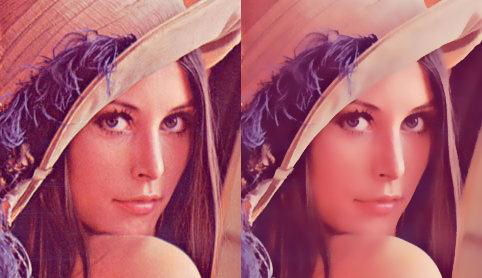
\includegraphics[width=0.6\textwidth]{./img/bilateral_filtering.jpg}
	\caption{A bilateral filter applied to a 2D color image.  The left is the original, while the right is filtered, resulting in removal of noise, figure adapted from \cite{pirovano2011kinfu}}.
	\label{fig:bilateralFiltering}
\end{figure}

If at time \(k\), the raw depth map \( R_k \) gives a depth measurement \( R_k(\textbf{u}) \) at image pixel \( \textbf{u} = (u,v)^T \) in the image domain \( \textbf{u} \in U \), then the bilateral filtered depth map \( D_k \) is given by:
\[  D_k(\textbf{u}) = \frac{1}{W_p} \sum_{\textbf{q} \in U}^{} \mathcal{N}_{\sigma_s}(\| \textbf{u} - \textbf{q} \|_2)  \mathcal{N}_{\sigma_r}(\| R_k(\textbf{u}) - R_k(\textbf{q}) \|_2) R_k(\textbf{q})  \]
, where 
\[ \mathcal{N}_{\sigma}(t) = exp(-t^2 \sigma^{-2}) \]
, and a normalizing constant 
\[  W_p = \sum_{\textbf{q} \in U}^{} \mathcal{N}_{\sigma_s}(\| \textbf{u} - \textbf{q} \|_2)  \mathcal{N}_{\sigma_r}(\| R_k(\textbf{u}) - R_k(\textbf{q}) \|_2)  \] 

After filtering, multiple resolutions of the depth frame is generated through sub-sampling, we call them the multi-resolution pyramid, illustrated by Figure \ref{fig:resolutionPyramid}.  Lastly, each layer of the pyramid generates a 3D point cloud through back projection using the camera's calibration matrix, \(\textbf{K}\), obtaining the point cloud (or vertex map) \(\textbf{V}_k\) in world coordinate,
\[  \textbf{V}_k(\textbf{u}) = D_k(\textbf{u}) \textbf{K}^{-1} \dot{\textbf{u}} \]
, where \( \dot{\textbf{u}} := (\textbf{u}^T|1)^T \)
\begin{figure} [h]
	\centering
	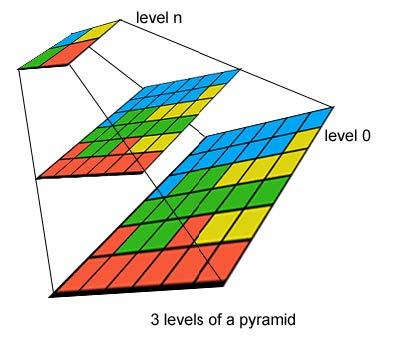
\includegraphics[width=0.6\textwidth]{./img/resolution_pyramid.jpg}
	\caption{A 3-level multi-resolution pyramid, figure adapted from \cite{pirovano2011kinfu}}.
	\label{fig:resolutionPyramid}
\end{figure}

In each point cloud, the normal for each point is estimated by an eigenvector of Principal Component Analysis (PCA) of its neighborhood points \cite{pirovano2011kinfu}.


\subparagraph{Alignment}
The preprocessed point clouds now need to be aligned to the current scene model.  If this is the very first depth frame, then its point cloud is used as the current model -- alignment starts at the second frame.  Alignment is done through the Iterative Closest Point (ICP) algorithm (with some modification of its procedures), starting from the point cloud of the coarsest layer in the pyramid.  ICP is performed in loops until one of the exit criteria is met, after which the same is done for the point cloud of the next level in the pyramid, and the next, until all levels are traversed.

The ICP loop (the modified version) has the following procedures:  Both points from the new frame's point cloud and the model's point cloud are projected to the model point cloud's camera image frame, and any pair of points from the two clouds falling onto the same pixel is noted as a match.  Then the rigid transform that globally minimizes the sum of squared errors between matched points is calculated, the error being the distance between the point of new cloud to the tangent plane of point of the model cloud, seen in Figure \ref{fig:pointToPlaneError} \cite{low2004linear}.
\begin{figure} [h]
	\centering
	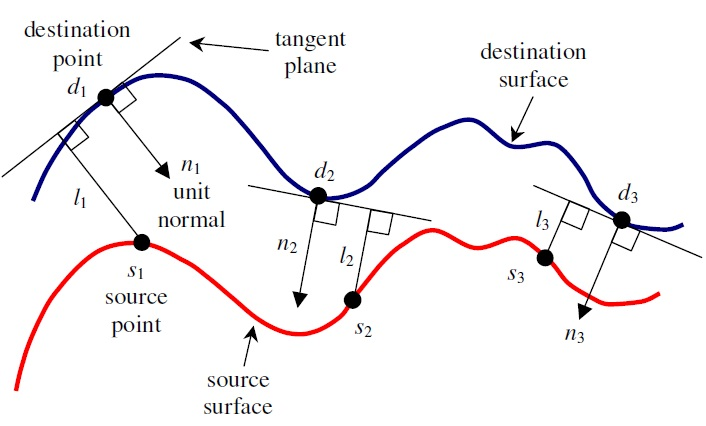
\includegraphics[width=0.6\textwidth]{./img/point_to_plane_error.jpg}
	\caption{Point-to-plane error between two surfaces, figure adapted from \cite{low2004linear}}.
	\label{fig:pointToPlaneError}
\end{figure}


If for a pair of points, \( \textbf{s}_i = (s_{ix}, s_{iy}, s_{iz}, 1)^T \) is the source point, \( \textbf{d}_i = (d_{ix}, d_{iy}, d_{iz}, 1)^T \) is the matched destination point, and \( \textbf{n}_i = (n_{ix}, n_{iy}, n_{iz}, 0)^T \) is the unit normal vector at \( \textbf{d}_i \), then in each ICP loop, the rigid-body transformation matrix \( \textbf{M} \) is found by
\[  \textbf{M}_{opt} = arg min_\textbf{M} \sum_{i}^{} ((\textbf{M} \cdot \textbf{s}_i - \textbf{d}_i) \cdot \textbf{n}_i)^2  \]

The exit criteria for the ICP loop are either 1) the maximum number of iterations are reached, 2) the changes of the transformation matrix falls below threshold, or 3) the sum of squared errors fall below threshold.

\subparagraph{Surface Reconstruction}
Finally, the aligned new frame needs to be integrated into the model and to form a new model point cloud so the pipeline can loop from the top as frames arrive.  A new model point cloud is formed by first converting the two clouds into Truncated Signed Distance Functions (TSDF).  A TSDF is basically a representation of surfaces of objects in a scene, with negative values assigned to voxels inside the surface or voxels that are not measured yet, positive values assigned to voxels outside the surface, increasing in value as we move further away from the surface, and voxels on the surface of objects are assigned the value of zero, illustrated in Figure \ref{fig:TSDF} \cite{newcombe2011kinectfusion}.  Here the raw value of the new frame with no filtering is used for calculating its TSDF to avoid losing details.
\begin{figure} [h]
	\centering
	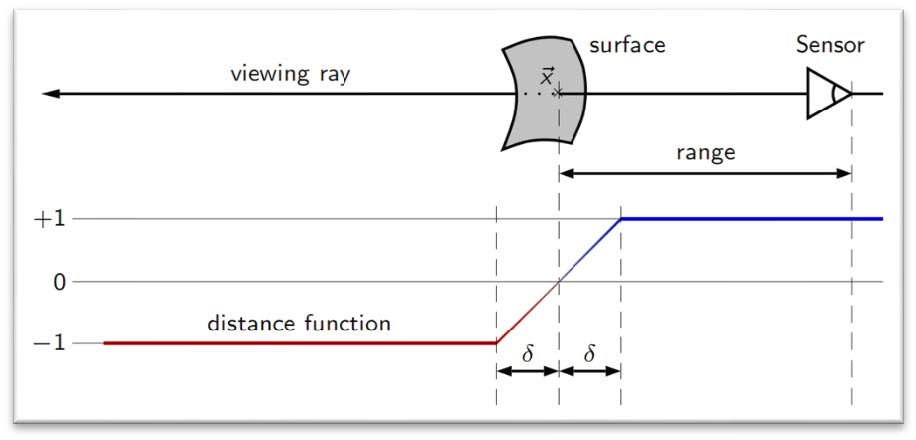
\includegraphics[width=0.6\textwidth]{./img/TSDF.jpg}
	\caption{A illustration of creating an 1D TSDF, figure adapted from \cite{pirovano2011kinfu}}.
	\label{fig:TSDF}
\end{figure}

Specifically, at a point \(\textbf{p}\) in the world coordinate, its projected nearest pixel \(\textbf{x}\) in the depth frame is given by,
\[  \textbf{x} = \lfloor \pi (\textbf{K} \textbf{M}^{-1}_{k} \textbf{p}) \rfloor  \]
, where \( \lfloor.\rfloor \) is the nearest neighbor lookup, and \( \textbf{q} = \pi(\textbf{p}) \) performs perspective projection of \(\textbf{p} = (x,y,z)^T\) with dehomogenization to obtain \(\textbf{q} = (x/z, y/z)^T\).

The TSDF \(F_{R_k}\) of a depth frame \(R_k\) at point \(\textbf{p}\) is computed as,
\[  F_{R_k}(\textbf{p}) = \Psi(\lambda^{-1}\|\textbf{t}_k - \textbf{p}\|_2 - R_k(\textbf{x}))  \]
, \[  \lambda = \|\textbf{K}^{-1} \dot{\textbf{x}} \|_2   \]
, 
\[
\Psi(\zeta) = 
\begin{cases}
min(1, \frac{\zeta}{\mu}) sgn(\zeta)  & \text{iff}\ \zeta \geq -\mu \\
\text{null} & \text{otherwise}
\end{cases}
\]
, where \(\textbf{t}\) is the translation part of the rigid body transformation matrix,
\[  \textbf{M} = 
\begin{bmatrix}
\textbf{R}		&	\textbf{t} \\
\textbf{0}^T	&	1
\end{bmatrix}  \]
, and \(\lambda^{-1}\) converts ray distance from frame origin to \(\textbf{p}\) to a depth value, and \(\Psi(.)\) truncates the SDF to a tolerance \(\mu\) within which distance to the uncertain depth measurement we expect the true value to lie.

After obtaining the TSDFs of the two clouds, volume integration of the two clouds are achieved by a weighted running average of the model cloud's TSDF with the new frame cloud's TSDF.
If the model before integration has TSDF \(F_{k-1}\), then integrating the new frame's TSDF \(F_{R_k}\) gives
\[  F_k(\textbf{p}) = \frac{W_{k-1}(\textbf{p}) F_{k-1}(\textbf{p}) + W_{R_k}(\textbf{p}) F_{R_k}(\textbf{p})} {W_k(\textbf{p})}   \]
\[  W_k(\textbf{p}) = W_{k-1}(\textbf{p}) + W_{R_k}(\textbf{p})  \]
, where \( W_{R_k}(\textbf{p}) \)is the weight used for correcting noisy measurements due to distance from sensor center, and is proportional to \( cos(\theta)/R_k(\textbf{x}) \), \(\theta\) the angle between the direction of the associated pixel ray and the surface normal.

Lastly, surface reconstruction is done through the marching cube algorithm, which converts the new model's TSDF into a point cloud.


%http://research.microsoft.com/pubs/155378/ismar2011.pdf
%http://homes.di.unimi.it/~pirovano/pdf/3d-scanning-pcl.pdf
%http://pointclouds.org/documentation/tutorials/normal_estimation.php

%- KinFu
%	- noise removal via bilateral filtering
%	- creation of multi-resolution pyramid (through sub-sampling)
%	- forming 3D point cloud (through back projection using cameras' calibration matrix) and normal estimation (through eigenvalue estimation) for each layer
%	- alignment (through ICP)
%		- for each point, search, within predefined radius, for its closest point
%		- calculate the rigid transform that minimizes sum of squared distances of all point pairs
%		- repeat this process until
%			- maximum number of iterations reached
%			- difference in transformations fall below threshold
%			- sum of squared distances fall below threshold
%		- KinFu makes modification:
%			- assumes small difference between frames!
%			- in order to parallelize computation, instead of searching for closest point in 3D space, it projects the two clouds onto the first cloud's camera image frame (2D), and pair all points that fall onto the same pixels.
%			- loops through ICP algorithm starting with coarser point clouds first, and works its way down the pyramid
%			- uses point to plane distance metrics instead of point to point, converging faster		
%	- surface reconstruction (through TSDF (Truncated Signed Distance Function) volume integration and marching cube surface reconstruction)
%		- raw depth data is used for merging into model instead of the filtered ones to avoid losing details
%		- calculate TSDF of current model and the new cloud to be merged
%		- merge the two TSDFs using weighted running average
%		- marching cube for reconstructing surface of the updated model's TSDF, creating a smoother point cloud with normals for registering next frame using ICP

\paragraph{Using KinFu with Kinect2 Camera}
To use KinFu with Kinect2 Camera, the open source PCL Kinect2 SDK and PCL Kinect2 KinFu by Steven Hickson (available on GitHub.com) are used.  They act as a driver for Kinect2 camera using the PCL point cloud framework.  This SDK currently only supports generating 3D non-color point cloud from the depth frames of Kinect2.  We had to implement the generation of color point cloud using the color frames ourselves.  However, the advantage of using this over using Microsoft Kinect2 for Windows SDK is that: first, Kinect Fusion was only in an unstable beta version in the Windows SDK during the time this thesis was conducted; second, the open source nature of PCL's KinFu enables us to have much more control in using the algorithm for our application.  The modifications to the KinFu algorithm are outlined in the sections following.


\paragraph{Using KinFu for Head Modeling}
Using KinFu for head modeling is very similar to the original purpose of KinFu -- scene modeling.  The difference lies that, for object (e.g. a head) modeling, we need to filter everything except the object of interest in the depth frame, so that KinFu only builds the 3D model over data on the object, and ignores everything.  One thing that's neat about object modeling is, instead of rotating the Kinect camera around the object, we can rotate the object while fixing the camera.  Also, specifically for head modeling, we can utilize Kinect's Skeleton Tracking algorithm to filter out everything except the head.

Not all objects can be tracked using the ICP algorithm in KinFu.  In KinFu's paper, the author reports that whenever the object is moving too quickly or when not enough 3D features (e.g. edges and corners) are present on the object surface, ICP often fails \cite{pirovano2011kinfu}.  This is mainly due to the assumption in ICP that between frame movements are small (note that this problem may be potentially solved by higher frame rate camera with higher computational power so no frames are skipped).  However, for head tracking, KinFu turns out to work just fine as long as the person isn't moving his/her head too fast.  Shown in Figure \ref{fig:headTrackingResults} (b) is an example 3D mesh model created using the above method.
\begin{figure} [h]
	\centering
	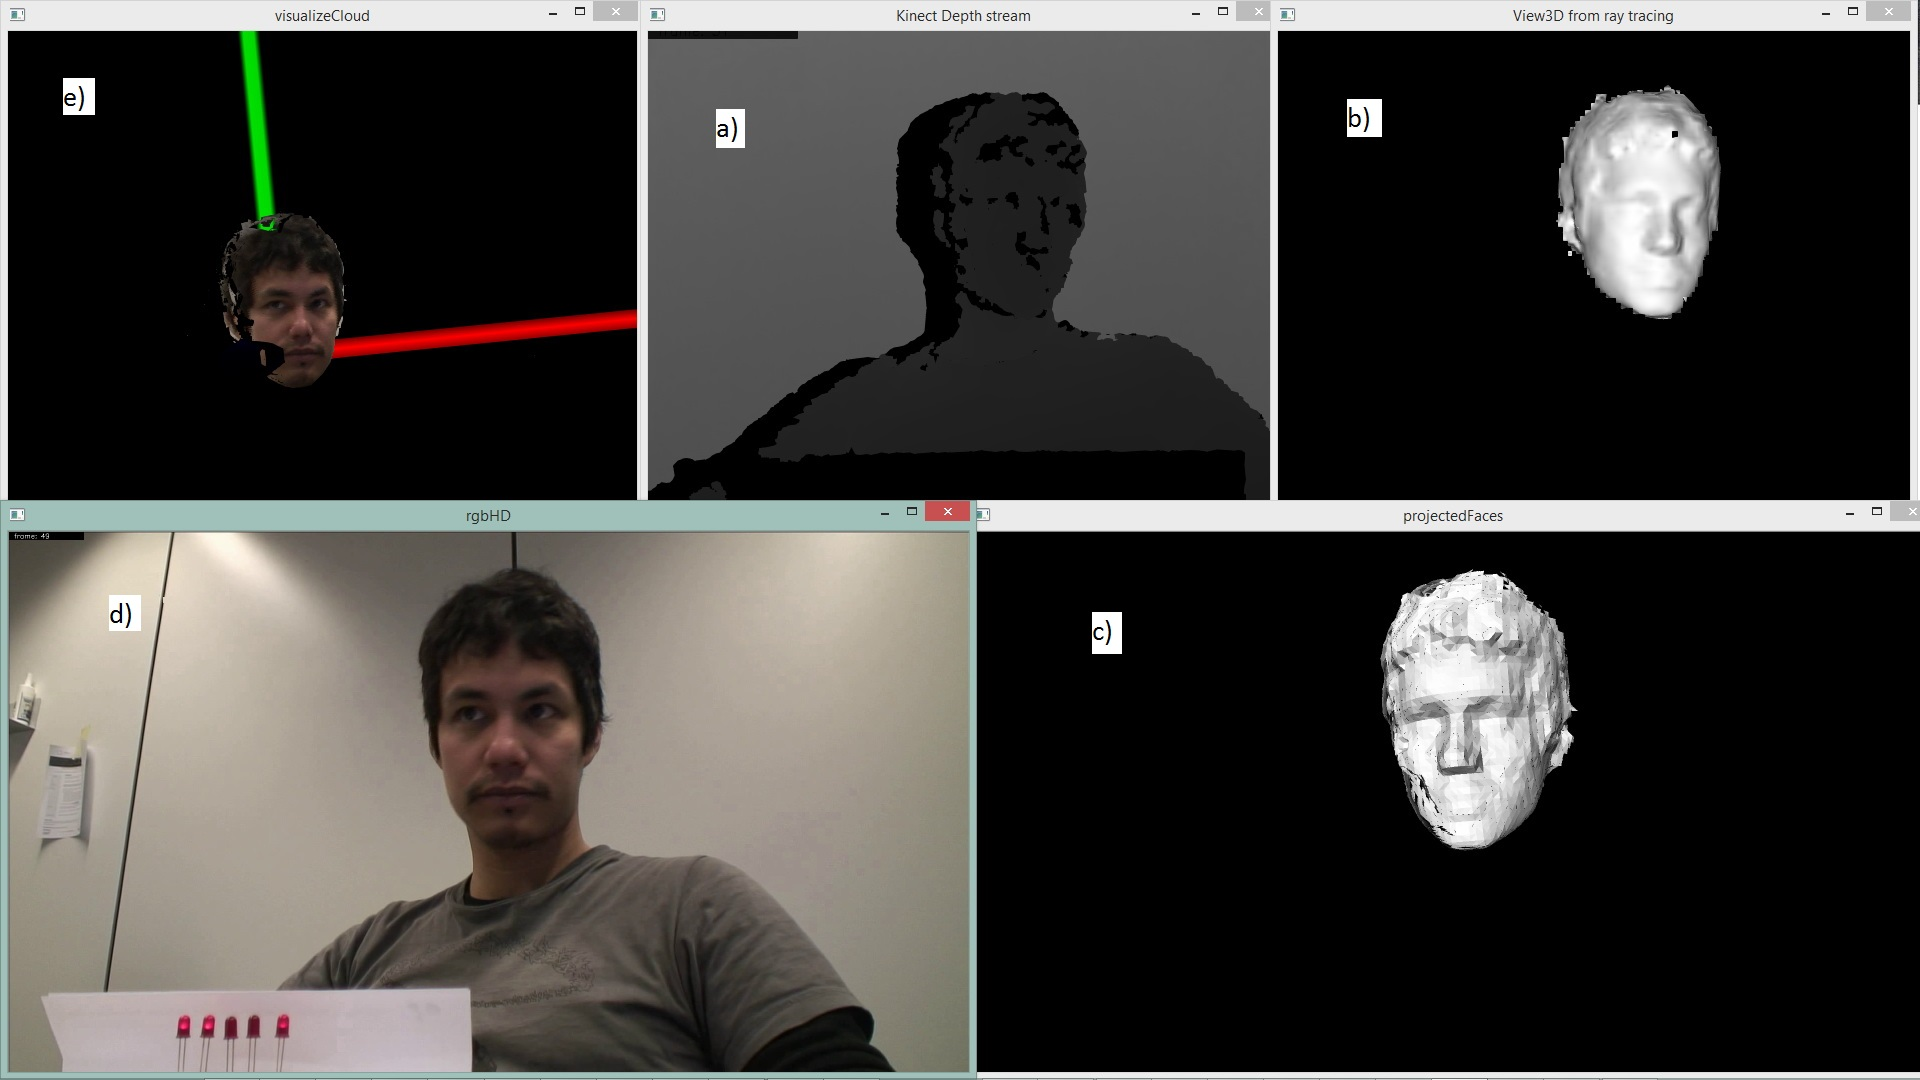
\includegraphics[width=\textwidth]{./img/headTrackingResults1.jpg}
	\caption{The 3D Kinect Camera Approach Results: we start by grabbing a frame from the Kinect depth camera (a), then we fit the 3D head model to the depth frame (b), after which we project the head model mesh onto the color camera image plane (c), so as to associate the color pixels with the head model mesh (d), and lastly forming the 3D color point cloud (e).}
	\label{fig:headTrackingResults}
\end{figure}

Also, facial expressions deform the face, making it deviate from the learned head model, and tracking accuracy may suffer due to the ICP's rigid nature.  Thus we see that the robustness of ICP head tracking depends on two factors:
\begin{itemize}
	\item the head's movement speed (both translational and rotational) relative to the ICP loop process speed or the Kinect camera's frame rate (which ever is the bottleneck)
	\item the dynamics of facial expressions on the head
\end{itemize}

%An evaluation of KinFu's capability for head modeling can be done by finding the maximum movement speed of the head (both translational and rotational) under expressionless vs. moving jaw faces conditions before KinFu's alignment step fails.  However, due to limitation of time, the algorithm's capability was not evaluated.


\subsubsection{KinFu Head Pose Tracking}
The KinFu algorithm was not been designed to be used for head pose tracking.  After obtaining the user's 3D head model, a few modifications to the algorithm was needed by the researcher so that the 3D position and pose (pitch, yaw, and roll) of the head can be tracked in the depth video stream using KinFu.  First, Skeleton Tracking is again used to filter out everything except the head in the depth video stream.  In addition, it is used to give initial position of head for the ICP loop, so that new frames to be aligned are within the capability of ICP.  Also, the KinFu algorithm needs to be modified to skip the surface reconstruction step, since we already have a model of the head.

%A similar evaluation of algorithm capability as mentioned above for KinFu head modeling can be done to see KinFu's robustness in head tracking.  However, this was not conducted due to time limitations.


\subsubsection{Point Cloud Based Inverse Pose Transformation}
Having accurate head model and head pose tracking enable us to restore the color image frames of the user's head into frontal pose.  The researcher implemented the processing scripts in C++ using the algorithms provided by the Point Cloud Library.  This inverse pose transformation is done by first forming a colored point cloud from the color frame, then 3D rigid transforming the point cloud inversely to the head pose so that the head represented by the point cloud is in frontal pose, finally projecting the transformed point cloud onto the camera image plane to obtain the 2D color image of the frontal posed head.

\paragraph{Colored Point Cloud}
To form a colored point cloud, we need to calculate the 3D coordinates of every pixel in the color frame.

The function "MapColorFrameToCameraSpace" provided by K4W SDK was originally for this purpose, and was used by the PCL Kinect2 KinFu SDK by Steven Hickson (the SDK's author).  However, MapColorFrameToCameraSpace provides the 3D coordinates of color pixels by associating each pixel in the color frame with a pixel in the depth frame, and then calculating the 3D coordinates of every pixel in the depth frame.  This approach is convenient to code and fast in execution, but is limited by the depth frame resolution.  For the typical resolution of the Kinect2 camera, the color frame resolution is 1920 X 1080 (2073600 pixels), the depth frame resolution is 512 X 424 (217088 pixels).  Using the above method, 2073600 pixels are available in color frame, but can only form 217088 unique points in the point cloud.  This is an order of magnitude reduction, wasting the HD color frame provided by the Kinect2 camera.  For Kinect1 camera, with color frame and depth resolutions being 640 X 480 (307200 pixels), this is also a huge reduction in resolution.  This problem of using the depth frame resolution for point cloud greatly reduces the resolution of the resulting frontal pose color image, making the next step, gaze prediction, less accurate if not much harder.

To avoid resolution reduction, the researcher implemented a new method of generating the color point cloud by using the 3D head model instead of the depth frame for calculating the 3D coordinates of each color pixel:

\subparagraph{Head Model Mesh Projection}
To do this, we first generate a triangular mesh version of the 3D head model.  Then we transform the head model mesh to match the pose in the current depth frame (done in previous step).  Next, we project the mesh onto the color camera image plane, keeping track of which pixel each vertex of the mesh lands on.  This enables us to mark which mesh surface each pixel in the projected image belongs to.  More specifically, for each mesh surface in the model, we do a depth first search traverse on the projected image starting with the pixel that one of the surface vertices projects to.  During traverse, we go to the pixel's neighbors one by one (there are eight adjacent neighbors to each pixel) if the pixel itself lies within the projected surface (i.e. inside the triangle formed by the surface's three projected vertices), and stop traversing if the pixel is outside of the projected surface, outside of the image boundary , or is already visited by the traverse.  There are times where two surfaces overlap in their projections -- this happens when one surface obstructs the view of the other (from the camera's point of view).  We handle this by assigning pixels to belong to the mesh surface nearest to the camera's focal point.  The result of this head model mesh projection is shown in Figure \ref{fig:headTrackingResults} (c).

\subparagraph{3D Coordinate Calculation}
After assigning surfaces to every pixel, the pixels' 3D coordinates can be calculated by linearly interpolating from the surface vertices.  To do this, we take advantage of the fact that Barycentric coordinates are preserved during projection of a planar object in 3D onto another plane.  Thus, a point on the 3D mesh surface preserves its Barycentric coordinate after projecting onto the color image plane.  Note that expressing a point in Barycentric coordinates w.r.t. a triangle it is on is basically expressing the point as a linear combination of two of the triangle's edges.  Mathematically, this means the following: Given triangular mesh surface vertices with coordinates P1, P2 and P3 in 3D, projected vertices with coordinates p1, p2 and p3 in 2D, and a point on the mesh surface with coordinate P in 3D, and projected coordinate p in 2D.  The Barycentric coorindate for P w.r.t. {P1, P2, P3} is \( (\lambda1, \lambda2, \lambda3)  \), with \( P = \lambda1 \times P1 + \lambda2 \times P2 + \lambda3 \times P3 \), \( \lambda1 + \lambda2 + \lambda3 = 1 \), and \( \lambda1, \lambda2, \lambda3 > 0 \).  Then, the Barycentric coorindate for the projected point, p, w.r.t. {p1, p2, p3} is also \( (\lambda1, \lambda2, \lambda3)  \), with \( p = \lambda1 \times p1 + \lambda2 \times p2 + \lambda3 \times p3 \).  Using this fact, we can calculate the Barycentric coordinate for each pixel w.r.t. the mesh surface it belongs to, and then calculate the pixel's back projected 3D coordinate using the surface's vertices' 3D coordinates.  An example of a colored point cloud formed using this method is shown in Figure \ref{fig:headTrackingResults} (e).

\paragraph{Inverse Pose Transformation}
With the color point cloud created, we are ready to form a frontal pose color image.  First, we rigid transform the cloud so that the center of the head is at coordinate (0, 0, 2 \( \times\) focal length) and its pose facing the origin.  The reason for 2 \( \times\) focal length is that the image plane is at 1 \( \times\) focal length, and we want the cloud to be a little distance away from the image plane so that the projection looks good inside the image boundaries.  Note that focal length is a programmer defined value used in the next step for perspective projection, and is the distance from image plane to the camera's focal point.

\subsubsection{Projection onto Camera Image Plane}
The last step before obtaining the frontal pose color image is the perspective projection.  For this, we go through every point in the color point cloud and calculate each point's 2D image coordinate.  If two points land in the same pixel, the one closer to the camera's focal point is used.  Several images of inverse pose transformed color point clouds projected onto the camera image plane are shown in Figure \ref{fig:inversePoseResults}.  We see that for moderate range of head poses, the algorithm works great.  However, at extreme range of head poses, distortions of the image and occlusions occur.  The distortion is mainly caused by the inaccuracy in head pose tracking as well as the crudeness of the 3D mesh head model (triangular mesh needs to be quite dense to approximate certain fine curves on the face, e.g. near the eyes).  The occlusion is a natural artifact due to lack of data from the RGB image.
\begin{figure}[h]
	\centering
	\begin{subfigure}[b]{0.32\textwidth}
		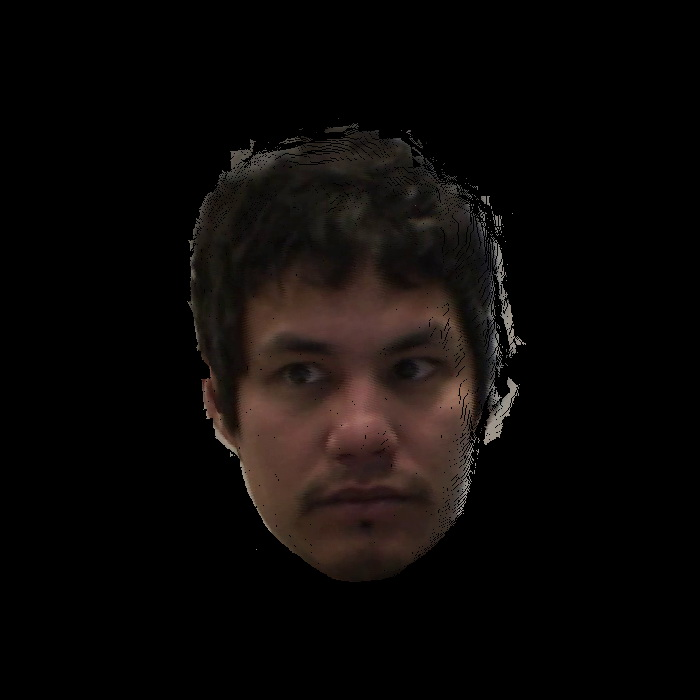
\includegraphics[width=1.1\linewidth]{./img/eyeimages/s1.jpg}
	\end{subfigure}
	\begin{subfigure}[b]{0.32\textwidth}
		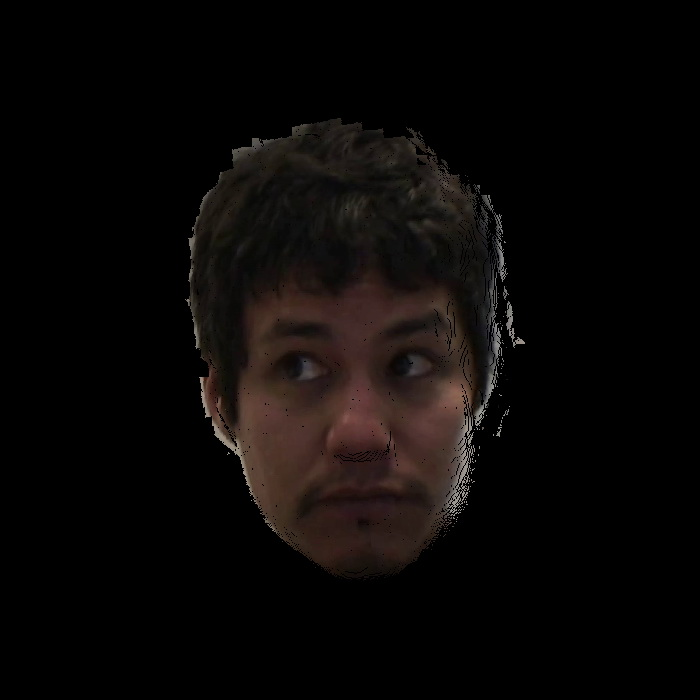
\includegraphics[width=1.1\linewidth]{./img/eyeimages/s2.jpg}
	\end{subfigure}
	\begin{subfigure}[b]{0.32\textwidth}
		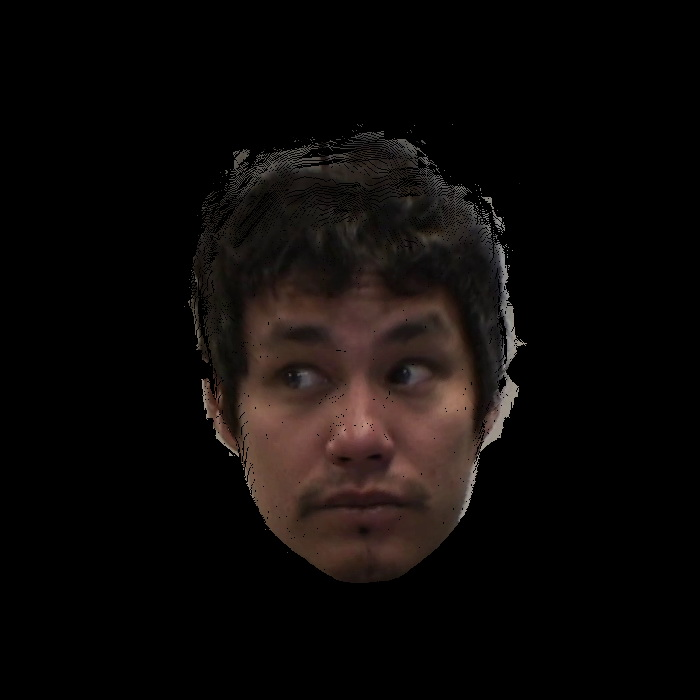
\includegraphics[width=1.1\linewidth]{./img/eyeimages/s3.jpg}
	\end{subfigure}
	\\
	\begin{subfigure}[b]{0.24\textwidth}
		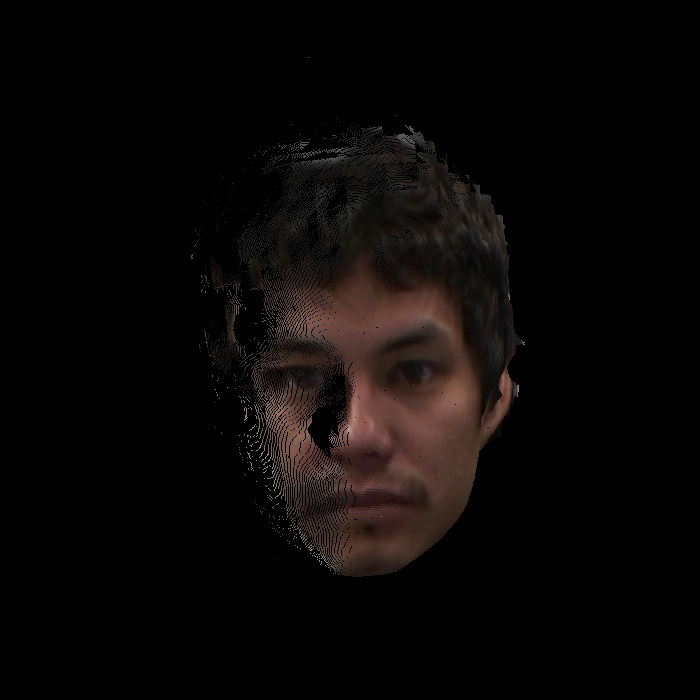
\includegraphics[width=1.1\linewidth]{./img/eyeimages/f1.jpg}
	\end{subfigure}
	\begin{subfigure}[b]{0.24\textwidth}
		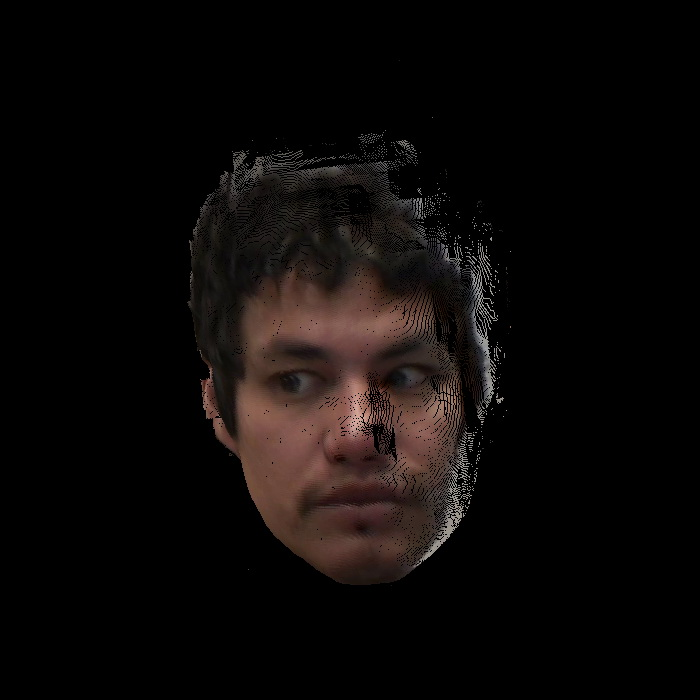
\includegraphics[width=1.1\linewidth]{./img/eyeimages/f2.jpg}
	\end{subfigure}
	\begin{subfigure}[b]{0.24\textwidth}
		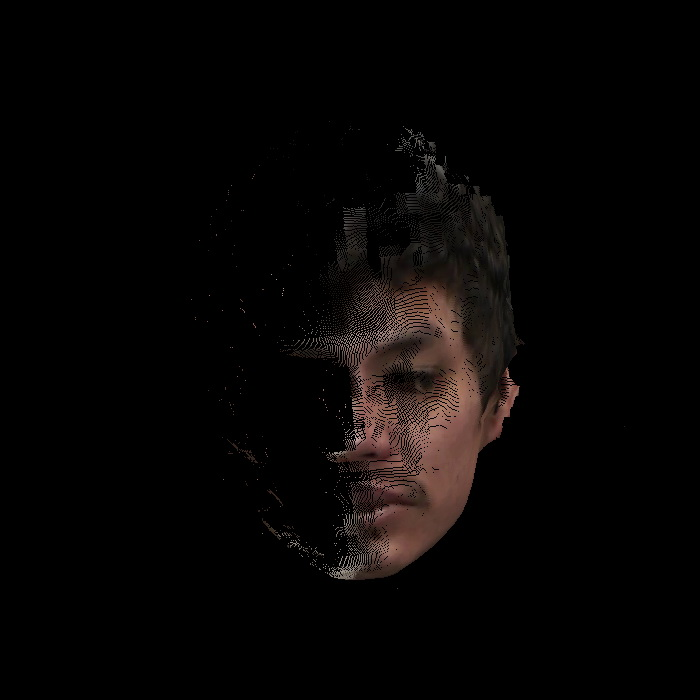
\includegraphics[width=1.1\linewidth]{./img/eyeimages/f3.jpg}
	\end{subfigure}
	\begin{subfigure}[b]{0.24\textwidth}
		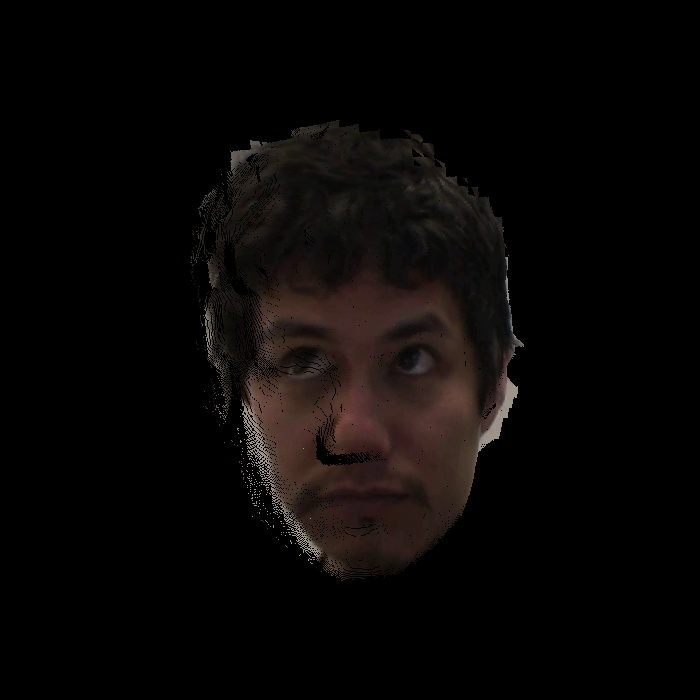
\includegraphics[width=1.1\linewidth]{./img/eyeimages/trackingError.jpg}
	\end{subfigure}
	\caption{Inverse Pose Transformed Color Images of an Example Head: The top row displays images of the head for moderate range of poses, showing little distortion and blank spots; the bottom row displays failure cases, the first three shows extreme head poses resulting in some distortions and huge blank spots due to occlusion, the last image shows a failure case due to head tracking error, resulting in large distortions.}
	\label{fig:inversePoseResults}
\end{figure}


There are pixels in the image that are blank because no points in the color point cloud landed on them.  When the cause of the blank spots is the point cloud being sparse, then the resulting projected image has scattered and small blank spots.  To this end, OpenCV's In-Painting algorithm is used to fill them \cite{bertalmio2000image}.  However, if the blank spots are caused by occlusion due to head pose, the spots are larger and more concentrated, and the In-Painting algorithm may be doing a poor job.  This only happens at the eye regions at extreme head poses, where other sources of distortion errors (e.g. head pose tracking inaccuracy) dominate.  Thus In-Painting being inaccurate in this case is tolerable, and treated as a limitation.

\subsubsection{Using the EYEDIAP Dataset}
Our ultimate goal is to predict the user's gaze given the depth and color video streams from Kinect.  So far, we are able to extract a frontal pose corrected color images of the eye regions.  The next step is to train a gaze predictor so the gaze direction can be predicted given a pair of eye region images.  To this end, we obtained the EYEDIAP Dataset online \cite{mora2014eyediap}.

The EYEDIAP Dataset was created by the IDIAP Research Institute for the purpose of training and evaluating gaze prediction algorithms using depth and color video streams.  It consists of 16 participants, 12 males and 4 females.  Participants are asked to gaze follow visual targets while being recorded by a Kinect1 camera and a HD video camera.  For each participant, three visual target conditions are recorded: target on a computer screen changing positions discretely, target on a computer screen changing positions continuously, and a small moving ball floated by a long pole moving continuously.  For each condition, two sessions are recorded, with one requiring the participant's head to remain still while the other allowing free movement.  The videos are annotated automatically for head pose and gaze direction.  This is done by using the 3D Morphable Model (3DMM) algorithm for head tracking, knowing the location of the visual targets on screen, and extracting the location of the floating ball target from the depth data.  Using the annotations, gaze predictors can be trained and evaluated.

To use the EYEDIAP Dataset in our framework, further modifications to the KinFu algorithm were made by the researcher.  First, instead of subscribing to the video sources of a Kinect camera, the depth and color videos of the dataset are read frame by frame using OpenCV.  Note that we are not using the Kinect1 camera's color videos; instead, the higher resolution HD camera videos are used along with the Kinect1's depth videos.  Depth frames are undistorted using the distortion calibration values provided, following the method used in the open source calibration toolbox by \cite{herrera2012joint}.  Also, image buffers' sizes are changed to match the HD video camera's resolution (1920 X 1080) and the Kinect1 depth camera's resolution (640 X 480).  Next, to form color point clouds, we need to map from depth frame's image coordinate to the world coordinate for forming the face model, and map from the world coordinate to the color frame's image coordinate for assigning mesh surfaces to color pixels.  These mappings are done by transforming the coordinates using the cameras' extrinsics and intrinsics provided.  During processing, the ICP alignment loop along with the color point cloud formation and projection reside in one thread, while the video frames grabbing reside in a separate thread.  Thus, synchronization is needed between threads to ensure no frame skipping when the processing thread is slow.  Lastly, Skeleton Tracking is only available if a dataset is recorded using Kinect Studio, thus it is not available in the EYEDIAP dataset.  Instead, we used in its place the 3DMM head pose tracking annotations by frame provided in the dataset.  We only used the translation part of the head tracking, and only needed it for initialization of ICP -- we still rely on ICP for orientation alignment in the first frame as well as full head pose tracking in new frames after that.

The results shown before (Figure \ref{fig:inversePoseResults}) were created using one of the video data in the EYEDIAP Dataset.

%How well does it perform?
%	- head modeling => not good for floating target and stationary head. => need moving head, DS or CS targets
%	- head tracking => fine for all three conditions?  how about moving vs stationary head?
%	- show results of eye regions cropped?



%\subsubsection{Evaluation On Child With ASD Videos}





\subsection{Eye Pose Estimation}

\subsubsection{Eye Image Cropping and Stabilization}
The appearance-based method we use follows after Mora et al. \cite{funes2013person}, and requires cropped eye images from frontal head pose.  As explained in previous section (Section \ref{sec:approachOverview}), the cropped color eye images are easily obtained as long as we have stable tracking of the head -- the relative position of the eyes on the head is unchanged although the head is moving.  Given the tracked head pose, we can reverse the viewing angle and project back the RGB image to obtain frontal head pose eye images.


\subsubsection{Eye Image Descriptor}
We first convert the eye image to gray-scale, normalize intensity values by setting mean to 125 and standard deviation to 30 (given that original intensity range is [0, 255]).  Then, we bin the image pixels into a grid of 3X5.  We form the descriptor e as the concatenated vector of bin values, normalized such that elements of e sum to 1.


\subsubsection{Adaptive Linear Regression (ALR)}
For a single eye, the gaze estimation problem can be formulated as the following: given training examples \( {(e_i,g_i )} \), input \(e'\), we want to estimate the gaze \(g'\).
Let \(E\) be the matrix whose \(i^{th}\) column i is \( e_i \), \(G\) be the matrix whose \(i^{th}\) column is \(g_i\), \(\epsilon\) be a tolerance parameter, we formulate our problem as a sparse reconstruction problem, finding the optimal \(w\) by minimizing the \(L_1\) norm of w:
\[ w' = argmin_w \|w\|_1  \quad  s.t.   \quad   \|Ew - e'\|_2 < \epsilon   \]
, then the estimated gaze \[ g' = Gw \]


\subsubsection{Coupled Eyes Constraints}
Now considering both eyes together, the ALR equation holds if we redefine the following:

\[  e = \begin{bmatrix}
e_l \\ e_r
\end{bmatrix}   \]

\[  w = \begin{bmatrix}
w_l \\ w_r
\end{bmatrix}   \]

\[  E = \begin{bmatrix}
E_l	&	0 \\
0	&	E_r
\end{bmatrix}  \]

and \[g = \begin{bmatrix}
g_{\phi l} \\ g_{\theta l} \\ g_{\phi r} \\ g_{\theta r}
\end{bmatrix}  \]
the vector of (pan, tilt) angles of the (left, right) eye

Then, the coupled eyes constraints can be formulated as: 
\begin{enumerate}
	\item Left and right eyes tilt angles should be the same:
	\[ g_{\phi l}^T w_l -  g_{\phi r}^T w_r = 0 \]
	
	\item Left and right eyes pan angles should not differ by more than a threshold, \(\tau_\phi\), with left eye the bigger angle
	\[  \tau_\phi < g_{\phi r}^T w_r - g_{\phi l}^T w_l < 0 \]
\end{enumerate}


\subsubsection{Solving ALR with Coupled Eyes Constraints}
The ALR with coupled eyes constraints can be solved as a Second Order Cone Programming problem \cite{funes2013person, kim2001second}.


\subsubsection{Training Examples Collection and Model Selection}
Since we are dealing with children with ASD, collecting person specific training examples would be infeasible.  Instead, generic training examples across multiple normal individuals are used.  Such training examples are extracted by cropping the eye regions from videos in the EYEDIAP dataset, with the ground truth gaze directions provided by the dataset.

After training examples are collected, eye pose estimation for a new person is done through ALR searching through the training examples.  We keep track of which person's training examples are used more often, and only keep the top few.  This is done by accumulating a running sum of \(w_i\) for each person.  This way, people that have eye appearances greatly differing from the new person are ignored, making the search more efficient and the estimation more accurate.
\section{Object Identification}
Given the gaze directions, in order to know which object is being looked at, we need to know the objects' locations.  We assumed that, in the future studies we are using this algorithm, object locations are fixed and their positions can be calibrate prior to the start of the study.  Here we present a object location calibration method implemented by the researcher.

The calibration should be performed by a person whose 3D head model has been learned and whose eyes are part of the ALR training examples for best gaze estimation accuracy.  The person is asked to look at each object when prompted while walking around, and gaze directions are estimated then recorded.  The intersection of two gaze directions pinpoints an object's location.  However, because the objects are larger than pinpoints, and gaze direction predictions have errors, thus we describe each object location as a Gaussian ellipsoid, with mean and variance calculated from all recorded gaze directions.  The resulting Gaussian ellipsoid is shown in Figure \ref{fig:locCalibResults}.  The center of the Gaussian, shown in red, is calculated by finding the point in space closest to all gaze lines, shown in blue.  For the \(i^{th}\) gaze line given by \(P_{oi} + s_i U_i\) (\(s_i\) a scalar, \(P_{oi}\) a 3D vector, and \(U_i\) a 3D unit vector), and for P the 3D point denoting the center to be calculated, then setting \(s_i = (P - P_{oi})\cdot{U_i} \) gives the closest point on the line to P (shown as green dots).  Our problem can be formulated as finding a P that minimizes the sum of squared distances between it and all lines:
\[ argmin_P \sum_{i}^{} || P_{oi} + [(P - P_{oi})\cdot{U_i}]U_i - P ||^2 \]
The solution to this is simply:
\[ P = [ \sum_{i}^{} I - U_i U_i^T ]^{-1}  [ \sum_{i}^{}(I - U_i U_i^T)P_{oi} ]   \]
The covariance of the Gaussian ellipsoid is given by calculating the covariance of the points


 Cov( \(P_{oi} + [(P - P_{oi})\cdot{U_i}]U_i\) )
 
\begin{figure}[h]
	\centering
	\begin{subfigure}[b]{0.49\textwidth}
		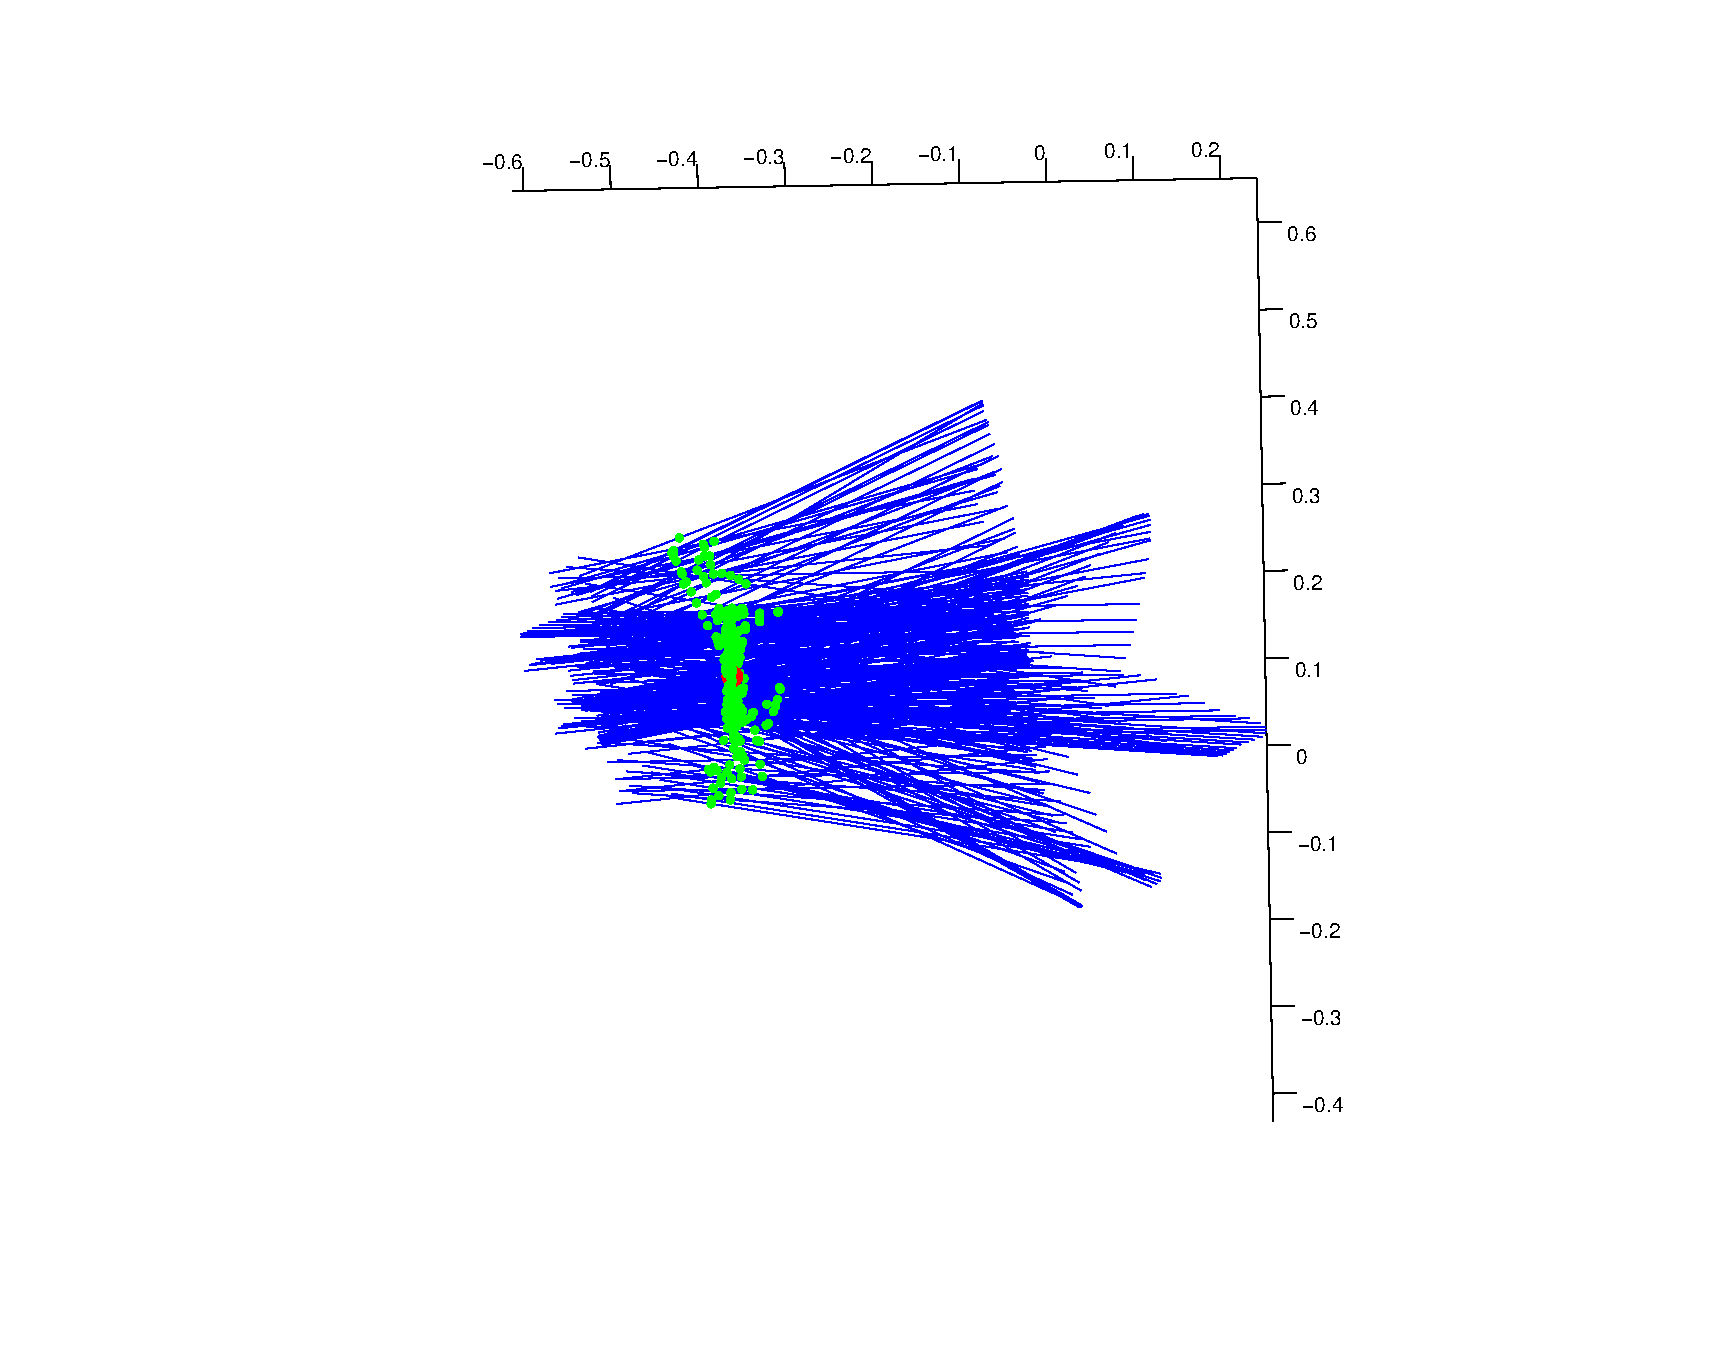
\includegraphics[width=1.1\linewidth]{./img/loc_calib_gauss.eps}
	\end{subfigure}
	\hfill
	\begin{subfigure}[b]{0.49\textwidth}
		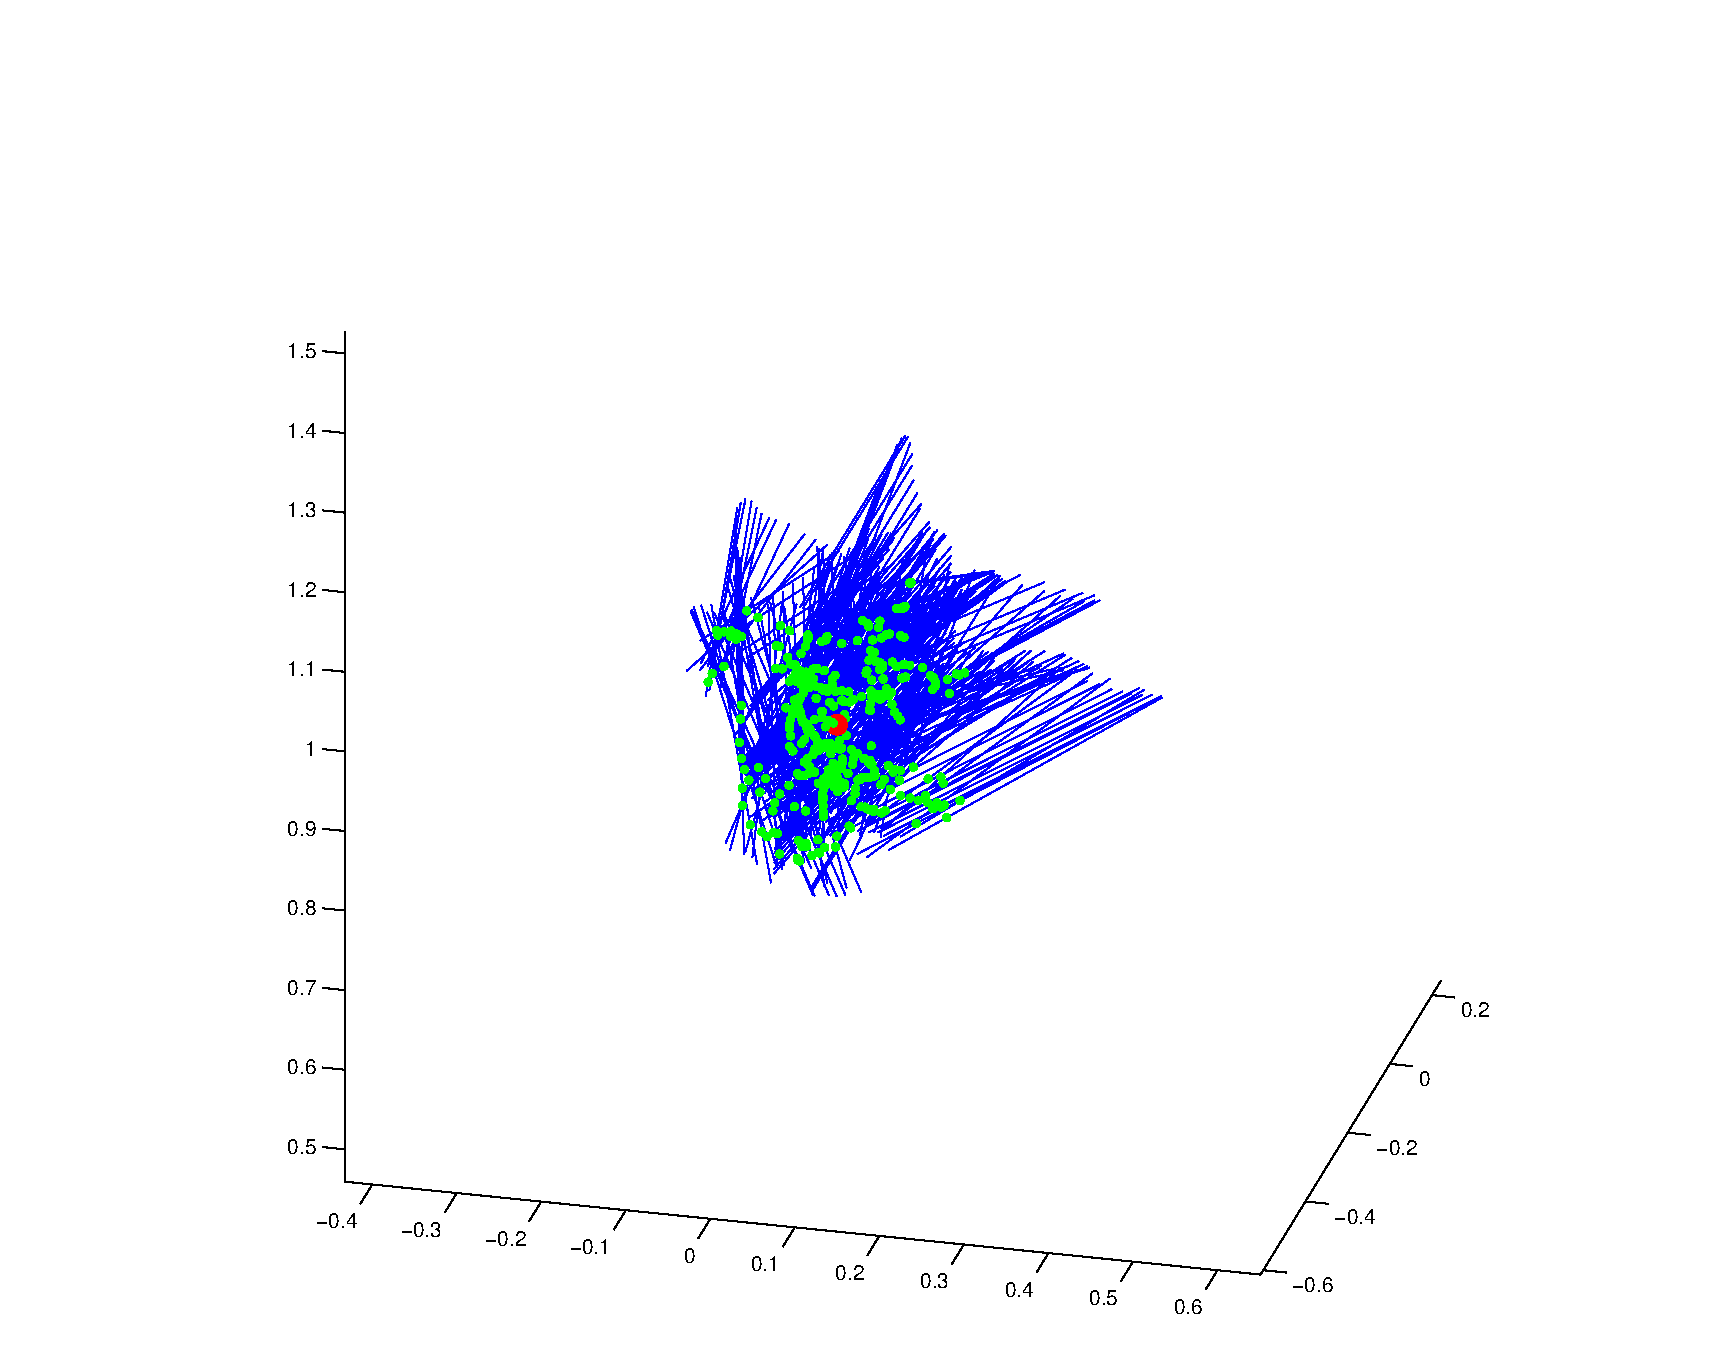
\includegraphics[width=1.1\linewidth]{./img/loc_calib_gauss_cross.eps}
	\end{subfigure}
	\caption{The Gaussian ellipsoid formed by finding the point of minimal sum of squared distances from all gaze lines.  Shown in red is the calculated point, shown in green are the closest point on each gaze line, shown in blue are the gaze lines.  In the left figure, the person doing the object location calibration is standing on the right, looking to the left.  The figure on the right shows the same plot rotated so the spread of the ellipsoid is seen more clearly.}
	\label{fig:locCalibResults}
\end{figure}

After this calibration for the objects of interest, we use a simple heuristic when identifying the object under gaze.  If gaze direction lies within x variance away from an object location mean, then this object is considered to be gazed at (x is a sensitivity parameter chosen manually).  If the gaze lies in two or more objects' vicinities, the object whose distance from gaze normalized by variance is less is chosen as the object under gaze.  If no objects are close to the gaze direction, the person is considered not looking at any object, i.e. idling.

\section{Discussion}
We have shown working implementations of the KinFu algorithm that produces inverse head pose transformed color eye images.  However, due to limitation of time, its capability was not explored.  We did test it with Kinect video footages we've obtained of the child with ASD's head during his hand-washing trials.  However, because the Kinect camera was placed too close to the participant's face (due to limitation of space near the sink), and because the participant rocks back and forth quite rapidly, our algorithm could not track the participant's head motions robustly.  Thus, we weren't able to build a head model from the footages, and thus further investigation was impeded.

For future studies, we need to first ensure the head tracker we developed works with children with ASD.  To do this, we should characterize children with ASD's head movement during hand-washing with the robot, since some children with ASD exhibit rocking motions.  We should note the speed and range of motions.  We may need to reposition the Kinect camera further away from the child to make sure the child's head motions does not go out of camera's range.  Then we need to characterize our head tracker's capability and make sure it can handle children with ASD's head movements.  If the head movements of children with ASD are faster than the tracker can handle, we may consider decreasing the number of vertices in the head model mesh to increase frame rate.

After obtaining a head tracker that works with children with ASD, we can move on to implementing the eye tracker.  Training eye images can be obtained by using the head tracker, doing the frontal pose transformation, and cropping the eye region using the EYEDIAP dataset.  Then the eye tracker can be implemented following the ALR method outlined previously.

For the future studies, one should evaluate the gaze (head plus eye) tracking accuracy for children with ASD.  One way to evaluate it is by letting children with ASD wear a commercially gaze tracking headset that gives the ground truth of their gaze, and compare it with the gaze direction estimated by our head plus eye tracker.  However, if asking children with ASD to wear the obtrusive headset proves to be infeasible, then maybe a fun activity can be designed that asks children with ASD to look at a moving object (e.g. a ball) whose 3D position can be automatically estimated using Kinect, serving as ground truth.

Lastly, the future studies should integrate the head and eye tracker with object under gaze estimator to realize the VFOA tracker, tracking the object under gaze in real-time.  Robot behaviors responding to child's gaze should then be implemented.  A study evaluating the effectiveness of implemented gaze behavior dependent robot actions on children with ASD's engagement, prompt compliance, and step completion during hand-washing prompting should be conducted.
\chapter{Conclusion}
In this thesis, we aimed to investigate a new prompting agent, humanoid robot NAO, for COACH during the prompting of hand-washing steps to a child with ASD.  A Wizard of Oz (WoZ) study was conducted, and yielded promising results.  In addition, we further improved COACH by attempting to implement a Visual Focus of Attention (VFOA) tracker.  The thesis answers the hypotheses raised in the following way (the hypotheses are shown in bold):

\paragraph{The humanoid robot, NAO, is able to independently assist child with ASD through hand-washing, and child exhibits greater engagement level, higher prompt compliance rate, and better task completion when prompted by NAO than by parent.}
Through the WoZ study, we have seen that NAO was effective in facilitating task completion in both variety and quality of steps, approaching the level of effectiveness achieved by the parent, but not better.  Also, NAO had a low prompt compliance rate compared to the parent during the first phase when it was introduced, but through a training phase of joint prompting with the parent, NAO resulted in a higher prompt compliance rate than before, comparable to that of the parent's.  We attribute the improvements of the robot effectiveness to the training phase, though several confounding variables such as learning effects, fatigue, and robot control were discussed.  In whole, although we have not achieved totally independent assistance using NAO, we have shown that NAO has very good potential of achieving independent assistance, given a longer and more intense training phase.

\paragraph{Gestural, gaze, and verbal are the essential modes of interactions present in the hand-washing prompting scenario between child with ASD and the prompting agent NAO.}
The WoZ study revealed that verbal instructions and pointing gestures are essential for a prompting agent to assist our participant, who knows the execution of each hand-washing step, but needs reminders of which step to execute.  In cases the child did need demonstrations for a step, NAO's limited dexterity as well as the slower motion speed of the motion demonstrations made it less effective compared to that of the parent's.  In addition, when the child is not complying, the parent increased the severity of the prompts, which the robot should implement in the future.  In terms of gaze behaviors during interactions, our participant generally avoided looking at the prompting agent when he knew what to do, and tends to look at the parent more than NAO when seeking help.  The child's gaze behavior was a poor indication of engagement.  Lastly, detection and understanding of verbal feedbacks from the child may be useful in predicting the engagement of our participant.

\paragraph{Using 3DMM and ALR for estimating head pose and eye pose, and using the Kinect camera, a classification rate of more than 80\% is achieved for estimating child's VFOA on NAO, monitor screen, soap, towel, tap region, hands, and idling.}
We have successfully completed a head pose tracker using the Kinect camera by modifying the KinFu algorithm.  However, due to rapid head movements of the participant during hand-washing sessions, our head pose tracker was not successful in tracking his head.  Future improvements were suggested.  We have also implemented frontal pose transformation of the head image for eye region cropping.  But due to limitation of time, we did not implement the eye pose tracker using EYEDIAP dataset employing the ALR method.  Lastly, we implemented the object under gaze estimator.  In whole, we showed the feasibility of implementing the VFOA's three components (i.e. head pose tracker, eye pose tracker, object under gaze estimator), and described the steps for completing its implementation and evaluating its performance.

\section{Significance}
In conclusion, the thesis results suggest promising prospects of utilizing the humanoid robot, NAO, as a novel prompting agent to enhance COACH, and to fill the gap of in-vivo ATCs for teaching daily skills to children with ASD.  Future investigations in regards to improving the child's engagement further through more creative design of the robot's appearance and behavior dynamics were suggested and explored.  One such improvement could come from implementing robot behaviors contingent to the VFOA of the child.

\section{Looking Back}
Looking back, there are several things we could have done differently to have a more successful thesis.

Before the start of the WoZ study, if the researcher had a deeper and clearer understanding of qualitative analysis in case studies, the iterative qualitative data collection and analysis could have been carried more rigorously and efficiently, and possibly more yielded more results.  Starting the WoZ study earlier so we were less time limited would have been really nice, too.  That would possibly longer training phase, and possibly yielding better results, even demonstrating the robot being as effective as the parent in prompting.  Also, having a few child alone hand-washing trials would be ideal, since we could use that opportunity to assess the child's habits and skills before starting the robot prompting trials, and less trials would be wasted in the operator adjusting the robot prompting to the child's preference.  The researcher practiced controlling the robot to prompt adult volunteers through hand-washing during the study preparation phase, but the adults were very nice and all wanted to follow the robot.  Certainly improvements were made to the robot through this, but what we really needed was to test the robot for dealing with noncompliance behaviors, and testing the robot with normal children would have been much effective in regard.

During the study results analysis, we carried out quantitative analysis first, only relying on intuitions on what measures make sense to analyze.  After that, we carried out qualitative analysis and found better measures for quantitative analysis, and thus the quantitative analyses were revised in light of this.  Instead, if we did qualitative analysis first, our intuitions of what measures to be analyzed quantitatively could have been founded in the qualitative results to begin with, saving time from much revisions.

For the technical contribution section of the thesis, instead of implementing a head pose tracker, an eye pose tracker, and an object identification algorithm, we should decrease the scope to head tracking only.  This way, we could have more time to properly evaluate the accuracy and robustness of the algorithm implemented.

%% This adds a line for the Bibliography in the Table of Contents.
\addcontentsline{toc}{chapter}{Bibliography}
%% *** Set the bibliography style. ***
%% (change according to your preference/requirements)
\bibliographystyle{plain}
%% *** Set the bibliography file. ***
%% ("thesis.bib" by default; change as needed)
\bibliography{./refs/thesis_report_refs}

%% *** NOTE ***
%% If you don't use bibliography files, comment out the previous line
%% and use \begin{thebibliography}...\end{thebibliography}.  (In that
%% case, you should probably put the bibliography in a separate file and
%% `\include' or `\input' it here).

\end{document}
